\chapter{Supplementary Material on Extragalactic Point Source Studies}

\section{Simulations of Extragalactic Gamma-ray Point Sources}
In this Appendix, we provide further details about the simulations and analyses of extragalactic point sources.

\subsection{Energy-Binned Source-Count Distributions}
\label{app:sims}

We generate simulated maps directly from the source-count distribution $dN/dF_{\gamma}$. To obtain this, we need two inputs: the gamma-ray luminosity function, $\Phi(L_{\gamma},z,\Gamma)$, and the source energy spectrum, $dF/dE$~\cite{DiMauro:2014wha}.  Typically, the luminosity function (LF) is given by
\begin{equation}
\Phi(L_{\gamma},z,\Gamma)=\frac{d^3N}{dL_\gamma\,dV\,d\Gamma} \,  ,
\end{equation}
where $V$ is the comoving volume, $\Gamma$ is the photon spectral index, $z$ is the redshift, $N$ is the number of sources, and $L_\gamma$ is the rest-frame luminosity for energies from 0.1--100~GeV in units of GeV\,s$^{-1}$.     

The photon flux in this energy range, $F_\gamma$, 
is defined in terms of the source energy spectrum,
\begin{equation}
F_\gamma(\Gamma) = \int_{E_\text{min}}^{E_\text{max}}\frac{dF}{dE} \, dE \, ,
\label{eq: Fgamma}
\end{equation}
where the units are cm$^{-2}$\,s$^{-1}$, and $E_\text{min(max)} = 0.1(100)$~GeV.

The source-count distribution is then given by
\begin{equation}
\frac{dN}{dF_\gamma} = \frac{1}{4\pi} \int_{\Gamma_\text{min}}^{\Gamma_\text{max}} d\Gamma \int_{z_\text{min}}^{z_\text{max}} dz \, \Phi(L_\gamma,z,\Gamma) \, \frac{dV}{dz} \, \frac{dL_\gamma}{dF_{\gamma}} \, ,
\label{eq: dNdFexact}
\end{equation}
which can be accurately estimated as
\begin{equation}
\frac{dN}{dF_\gamma} \approx \frac{1}{\Delta F_\gamma} \, \frac{1}{4\pi} \int_{\Gamma_\text{min}}^{\Gamma_\text{max}} d\Gamma \int_{z_\text{min}}^{z_\text{max}} dz \, \int_{L_\gamma(F_\gamma, \Gamma,z)}^{L_\gamma(F_\gamma+\Delta F_\gamma, \Gamma,z)} dL_\gamma \, \Phi(L_\gamma,z,\Gamma) \, \frac{dV}{dz} \, ,
\label{eq: dNdF}
\end{equation}
where $4\pi$ is the full-sky solid angle, $dV/dz$ is the comoving volume slice for a given redshift and $\Delta F_\gamma$ is sufficiently small.  To calculate $dN/dF_\gamma$, we need the following expression, which relates the luminosity to the energy flux:
\begin{equation} 
L_\gamma(F_\gamma, \Gamma,z) = \frac{4\pi d_L^2}{(1+z)^{2-\Gamma}}  \, \int_{E_\text{min}}^{E_\text{max}} \, E\,\frac{dF}{dE}\, dE \, ,
\label{eq:lumi}
\end{equation}
where $d_L$ is the luminosity distance. For a given $F_\gamma$ and $\Gamma$, one can use~\eqref{eq: Fgamma} to solve for the normalization of $dF/dE$, which can be substituted into~\eqref{eq:lumi}, along with $z$ and $\Gamma$, to obtain the associated value of the luminosity. The photon flux, $F_\gamma$, is related to the photon count, $S_\gamma$, via the mean exposure $\langle \bar{\mathcal{E}} \rangle$, which is averaged over 0.1--100~GeV and the ROI.  This allows us to finally obtain $dN/dS_\gamma$ from \eqref{eq: dNdF}.

The procedure outlined above allows one to obtain the source-count distributions based on models of luminosity functions and spectral energy distributions provided in the literature. For the AGN and SFG examples we consider in detail in this work, the luminosity functions correspond to photon energies from 0.1--100~GeV.  However, we also need the source-count distributions in subset energy ranges corresponding to our energy bins of interest, with $E'_\text{min, max}\in [0.1, 100]$~GeV.  We rescale the fluxes for these individual energy bins of interest to those in the provided 0.1--100~GeV range using a procedure similar to~\cite{DiMauro:2014wha}. Denoting quantities associated with this energy bin with a prime, we can write the new source-count distribution as
\begin{equation}
\frac{dN}{dF'_\gamma}\approx \frac{1}{\Delta F'_\gamma} \, \frac{1}{4\pi} \int_{\Gamma_\text{min}}^{\Gamma_\text{max}} d\Gamma \int_{z_\text{min}}^{z_\text{max}} dz \int_{L_\gamma(F_\gamma(F'_\gamma,\Gamma),\Gamma,z)}^{L_\gamma(F_\gamma(F'_\gamma+\Delta F'_\gamma,\Gamma),\Gamma,z)} dL_\gamma \, \Phi(L_\gamma,z,\Gamma) \, \frac{dV}{dz} \, ,
\label{eq: dNdFprime}
\end{equation}
where $\Delta F'_\gamma$ is again sufficiently small---we set $\Delta F'_\gamma \equiv 10^{-3} F'_\gamma$, and verify that the answer is robust to this choice. Note that the integral must still be done over $L_\gamma$ (unprimed) because the luminosity function is explicitly defined in terms of it.  So, we must solve for the photon flux over the full energy, $F_\gamma$, in terms of the value in the sub-bin, $F_\gamma'$.  The two are related via a proportionality relation
\begin{equation}
F_\gamma(F'_\gamma,\Gamma) = F'_\gamma \, \frac{\int_{E_\text{min}}^{E_\text{max}}  dE \int_{L_{\gamma,\text{min}}}^{L_{\gamma,\text{max}}} dL_{\gamma}\int_{z_\text{min}}^{z_\text{max}} dz \,  \Phi(L_\gamma,z,\Gamma) \, \frac{dV}{dz} \, \frac{dF}{dE}\,e^{-\tau_\text{\tiny{EBL}}(E,z)}}{\int_{E'_\text{min}}^{E'_\text{max}}  dE \int_{L_{\gamma,\text{min}}}^{L_{\gamma,\text{max}}} dL_{\gamma}\int_{z_\text{min}}^{z_\text{max}} dz \, \Phi(L_\gamma,z,\Gamma) \, \frac{dV}{dz} \, \frac{dF}{dE}\,e^{-\tau_\text{\tiny{EBL}}(E,z)}} \, ,
\end{equation}
where the exponential factor accounts for the attenuation due to extragalactic background light (EBL)~\cite{Gould:1966pza, Fazio:1970pr, 1992ApJ...390L..49S, Franceschini:2008tp, 2012Sci...338.1190A,Abramowski:2012ry,Dominguez:2013lfa}.  It arises from pair annihilation of high-energy gamma-ray photons with other background photons in infrared, optical, and/or ultraviolet, and is described by the optical depth, $\tau_\text{\tiny{EBL}}$.  We use the EBL attenuation model from~\cite{2010ApJ...712..238F}.  

Additionally, the expected gamma-ray spectrum can be calculated from the luminosity function as
\begin{equation}
\frac{dN}{dE} = \frac{1}{4\pi} \int_{\Gamma_\text{min}}^{\Gamma_\text{max}} d\Gamma \int_{z_\text{min}}^{z_\text{max}} dz \, \int_{L_{\gamma,\text{min}}}^{L_{\gamma,\text{max}}} dL_\gamma \, \Phi(L_\gamma,z,\Gamma) \, \frac{dV}{dz}\,\frac{dF}{dE} \, e^{-\tau_\text{\tiny{EBL}}(E,z)} \, .
\label{eq: dIdE}
\end{equation}
We use this equation to appropriately weight the number of photons per energy sub-bin for the individual sources when creating simulated maps. This ensures that the variations in PSF and exposure within the larger energy bins used in the NPTF analyses are properly accounted for in the simulation procedure.

\subsection{Simulations at Energies $\lesssim$ 1.89~GeV}
\label{app:verylowenergies}

The main analyses presented in the text do not consider energies below 1.89~GeV because we find that systematic effects may become more important at these low energies.  In particular, simulations done with the set of priors presented in Sec.~\ref{sec:methodology} show that the NPTF can over-estimate the PS intensity at very low energies.   
That is, in simulations with both blazars and SFGs, the isotropic-PS template tends to absorb more emission than is simulated in blazars, while the smooth isotropic template absorbs less emission than is simulated in SFGs.
 
As an illustration, we show the results when the NPTF is run on a simulated map of Blazar--1 and SFG sources.  Figure~\ref{fig:dnds_verylow} shows the best-fit source-count distributions for the energy ranges 0.475--0.753 and 0.753--1.89~GeV.  The PS fractions in these bins are $I_\text{iso}^\text{PS} / I_\text{blazar-sim} = [1.17_{-0.09}^{+0.13}, 1.26_{-0.08}^{+0.10}]$, illustrating that the PS template is absorbing more PS emission than is simulated in blazars.  From Fig.~\ref{fig:dnds_verylow}, we see that this is likely the result of the fit typically predicting more sources than it should at intermediate and low fluxes.  This could be due to a variety of factors.  For example, 
at very low energies the angular resolution of the detector quickly degrades, and the PS flux also becomes more and more sub-dominant compared to foreground emission.  For these reasons---and out of an abundance of caution---we do not present results of the NPTF on data below 1.89 GeV.  It is certainly possible that analyses at low energies could provide a wealth of interesting observations.  However, having confidence in the NPTF results at such low-energies requires a more careful consideration of systematics, which goes beyond the scope of the present work.  
\begin{figure*}[htbp] %  figure placement: here, top, bottom, or page
   	\begin{center}$
	\begin{array}{c}
	\scalebox{0.5}{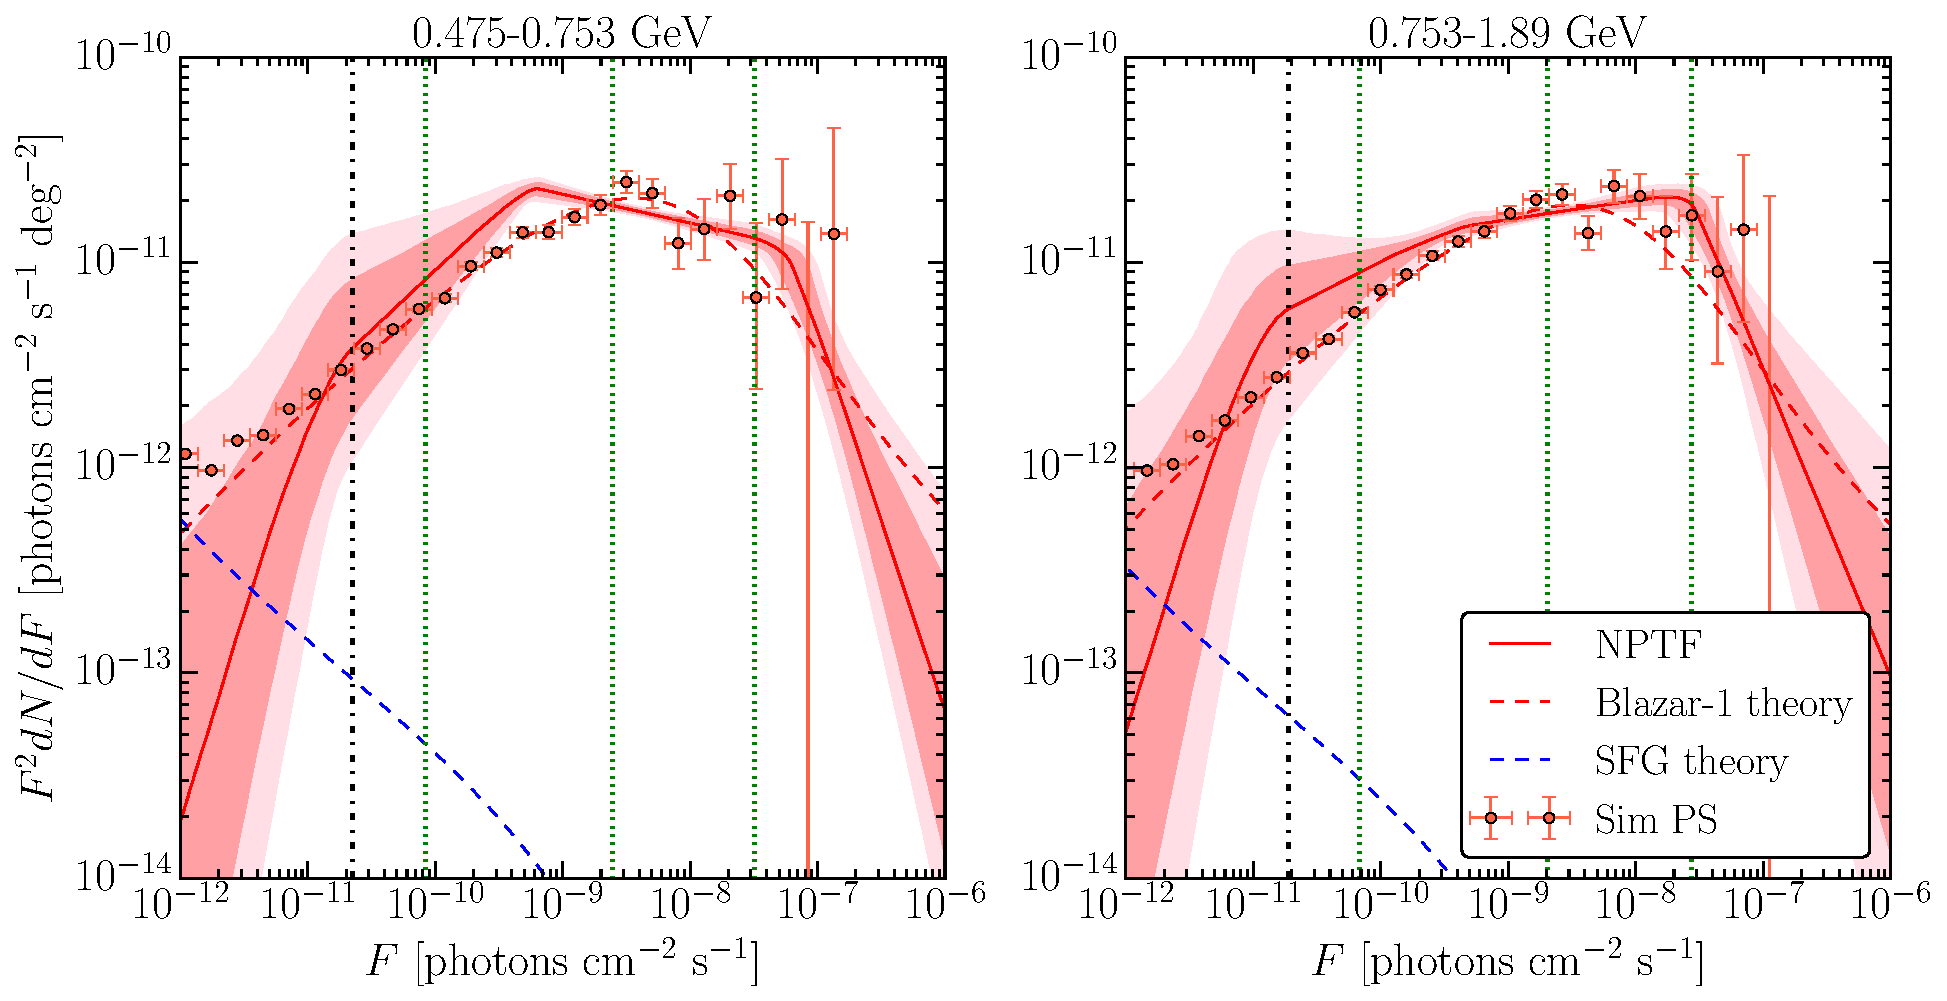
\includegraphics{ch-igrb/plots/bl1sf-lowE-dnds.pdf}} 
	\end{array}$
	\end{center}
\caption{Best-fit source-count distribution for a simulated map containing both Blazar--1 and SFG sources in the 0.475--0.753 \emph{(left)} and 0.753--1.89 \emph{(right)}~GeV energy bins.  (Formatted as in Fig.~\ref{fig:bl1dnds}.) }
   \label{fig:dnds_verylow} 
\end{figure*}

\clearpage
\subsection{{\it Ultracleanveto} PSF1-3 Simulation Analysis}
\label{app:ucvsims}

The simulated-data studies in the main text used the PSF3 instrument response function for the Pass~8 {\it ultracleanveto} data set.  Here, we show what happens when using the PSF1--3 instrument response function instead.  Including the top three quartiles of data increases the total exposure, though at the cost of decreased angular resolution.  Figure~\ref{fig:dndsb2UCV} illustrates the result for the Blazar--2 simulated data set.  The best-fit source-count distribution extends to lower fluxes than the corresponding distribution for top-quartile data in Fig.~\ref{fig:bl2dnds}. 

\begin{figure*}[b] %  figure placement: here, top, bottom, or page
   \centering
   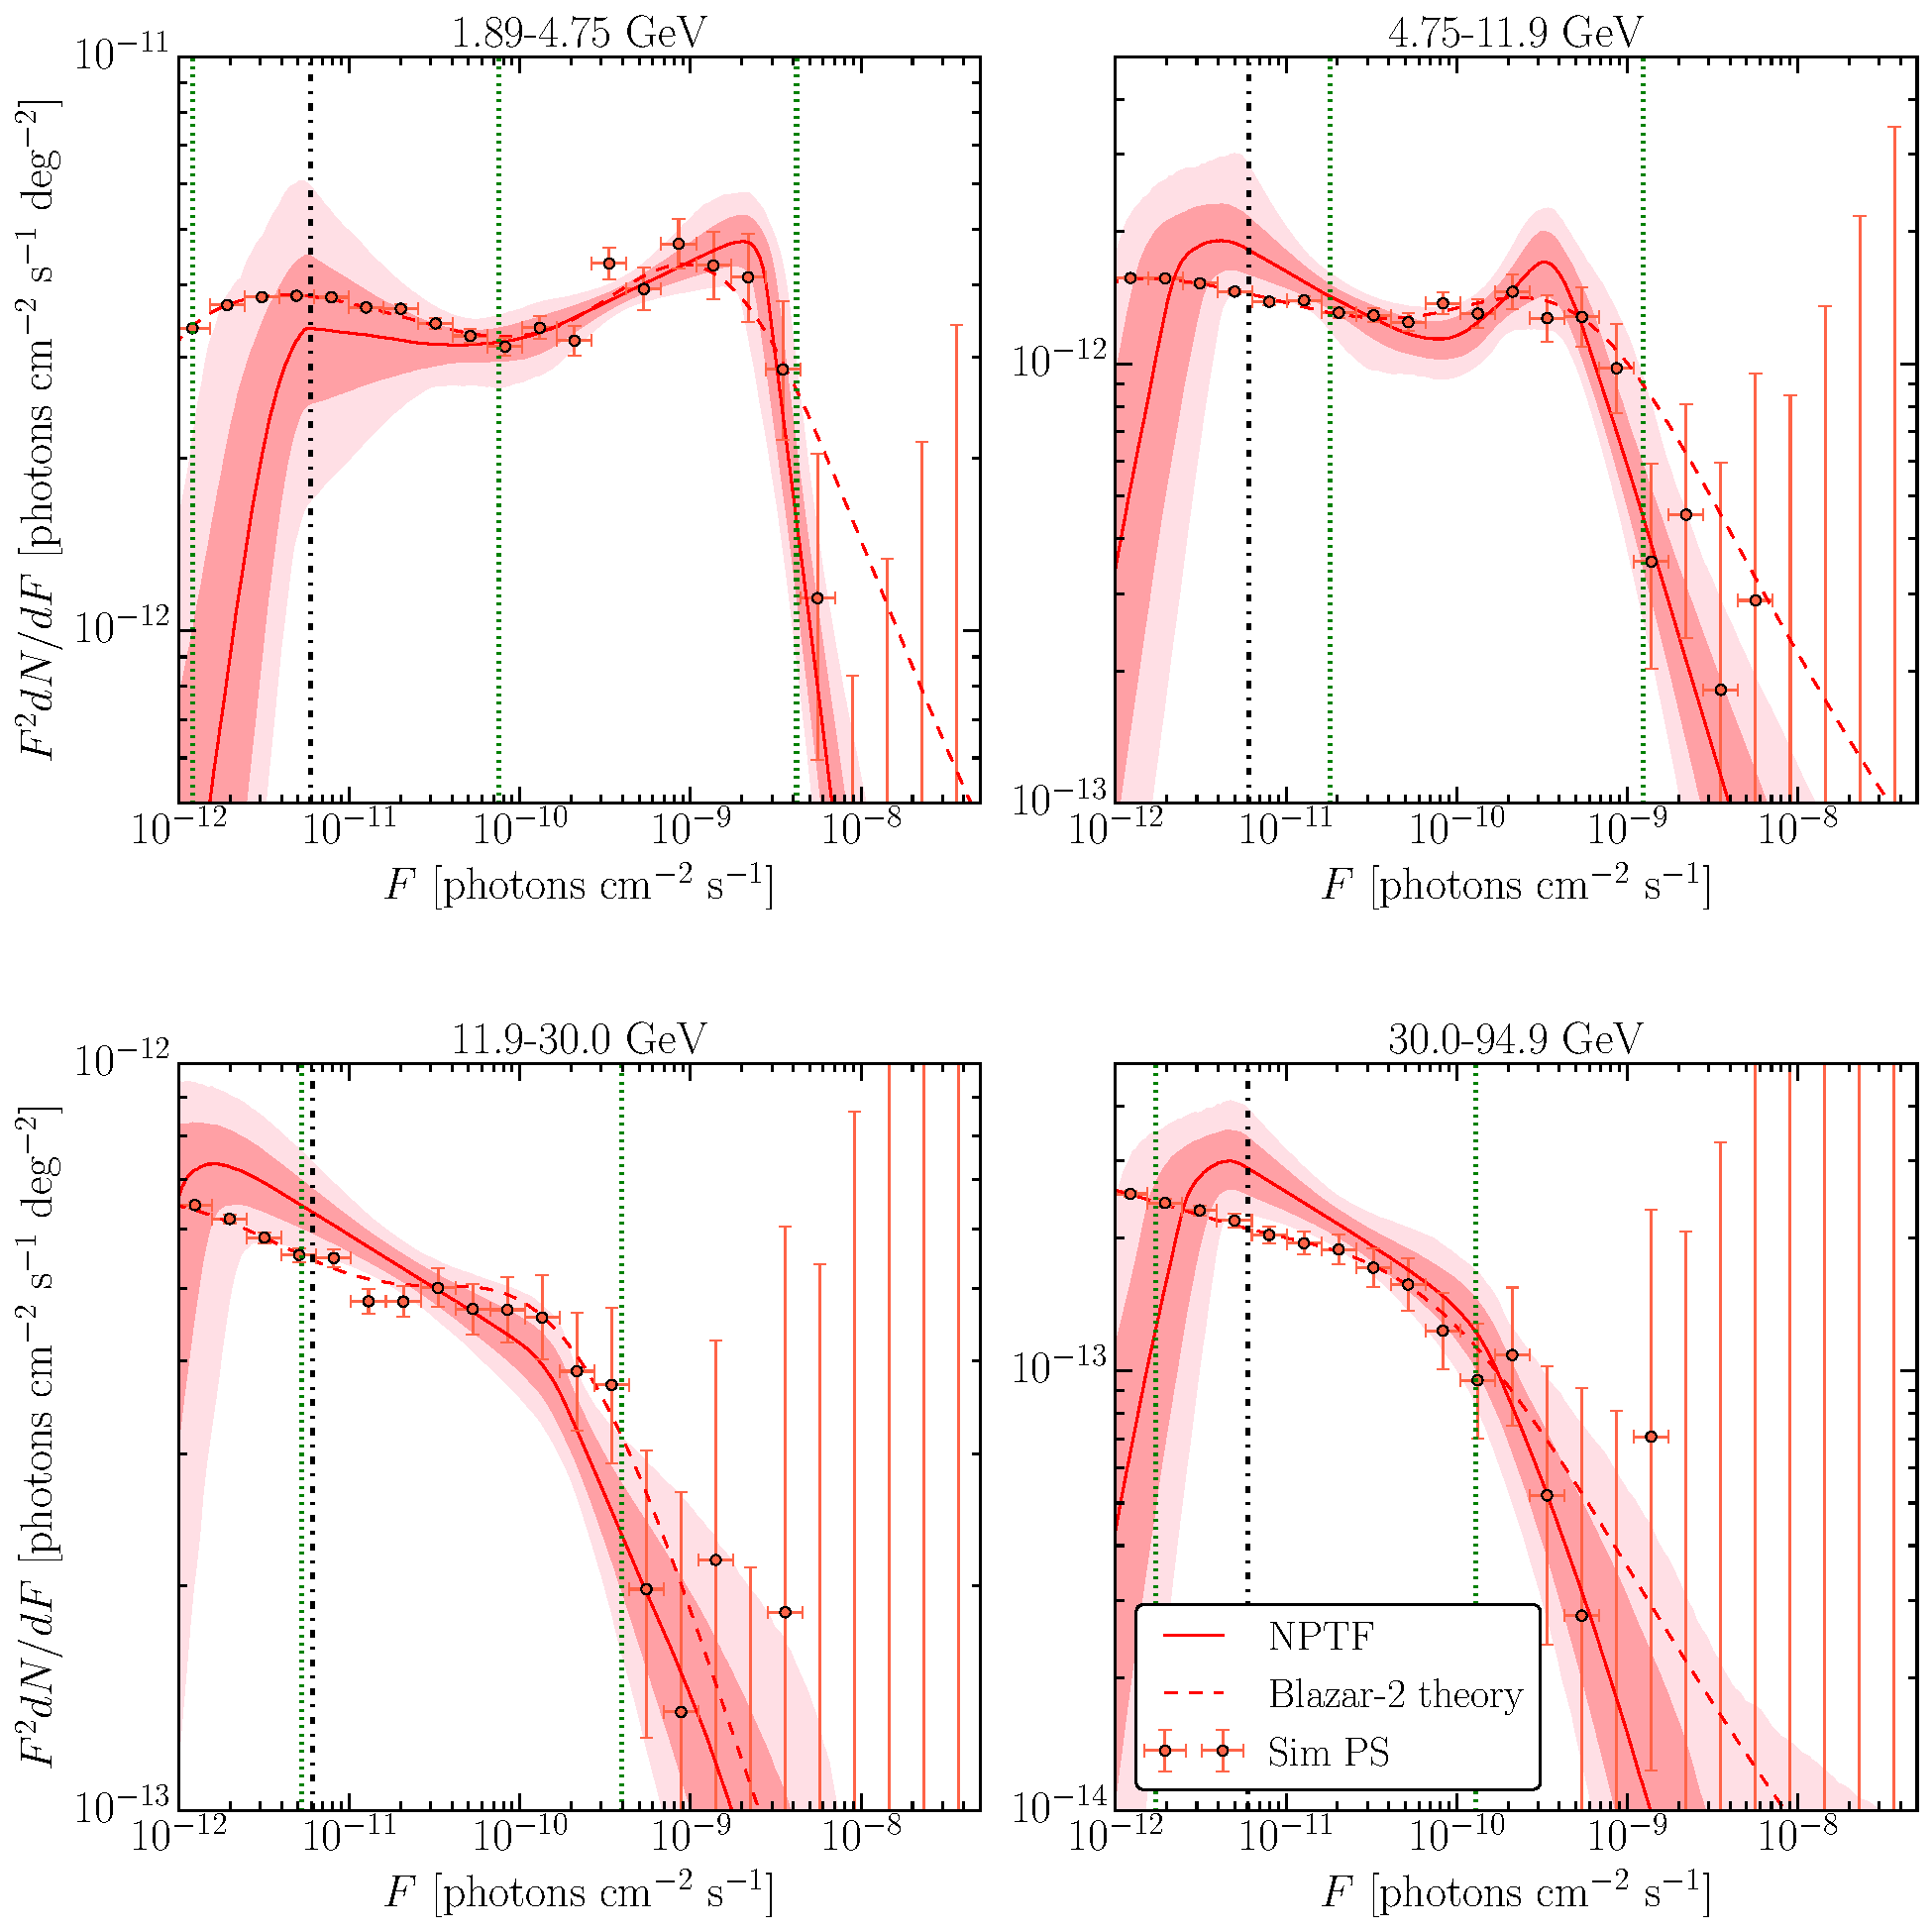
\includegraphics[width=\textwidth]{ch-igrb/plots/bl2-ucv-dnds.pdf} 
   \caption{Best-fit source-count distribution, as a function of energy, obtained from simulating the Blazar--2 model with top three quartiles of \emph{ultracleanveto} data.  (Formatted as in Fig.~\ref{fig:bl1dnds}.)}
   \label{fig:dndsb2UCV}
\end{figure*}


\subsection{Simulations of SFGs}
\label{app:sfgsims}

Here, we show the results of running the NPTF analysis on simulated data where the EGB arises solely from SFGs.  The resulting best-fit source-count distributions are shown in Fig.~\ref{fig:simdata_sfg}.  In the first energy bin, the brightest SFGs, which contribute little more than $\sim$1 photon, are detected as PSs by the NPTF.  At higher energies, the best-fit source-count distributions are consistent with zero and no significant evidence for a PS population is found.  The energy spectrum plot in Fig.~\ref{fig:spec_sfg} shows that the SFG flux is absorbed by the smooth isotropic template.  In comparison, the intensity absorbed by the isotropic-PS template is completely subdominant and is several orders of magnitude lower than its Poissonian counterpart at all energies.

\begin{figure}[b] %  figure placement: here, top, bottom, or page
   	\begin{center}$
	\begin{array}{c}
	\scalebox{0.5}{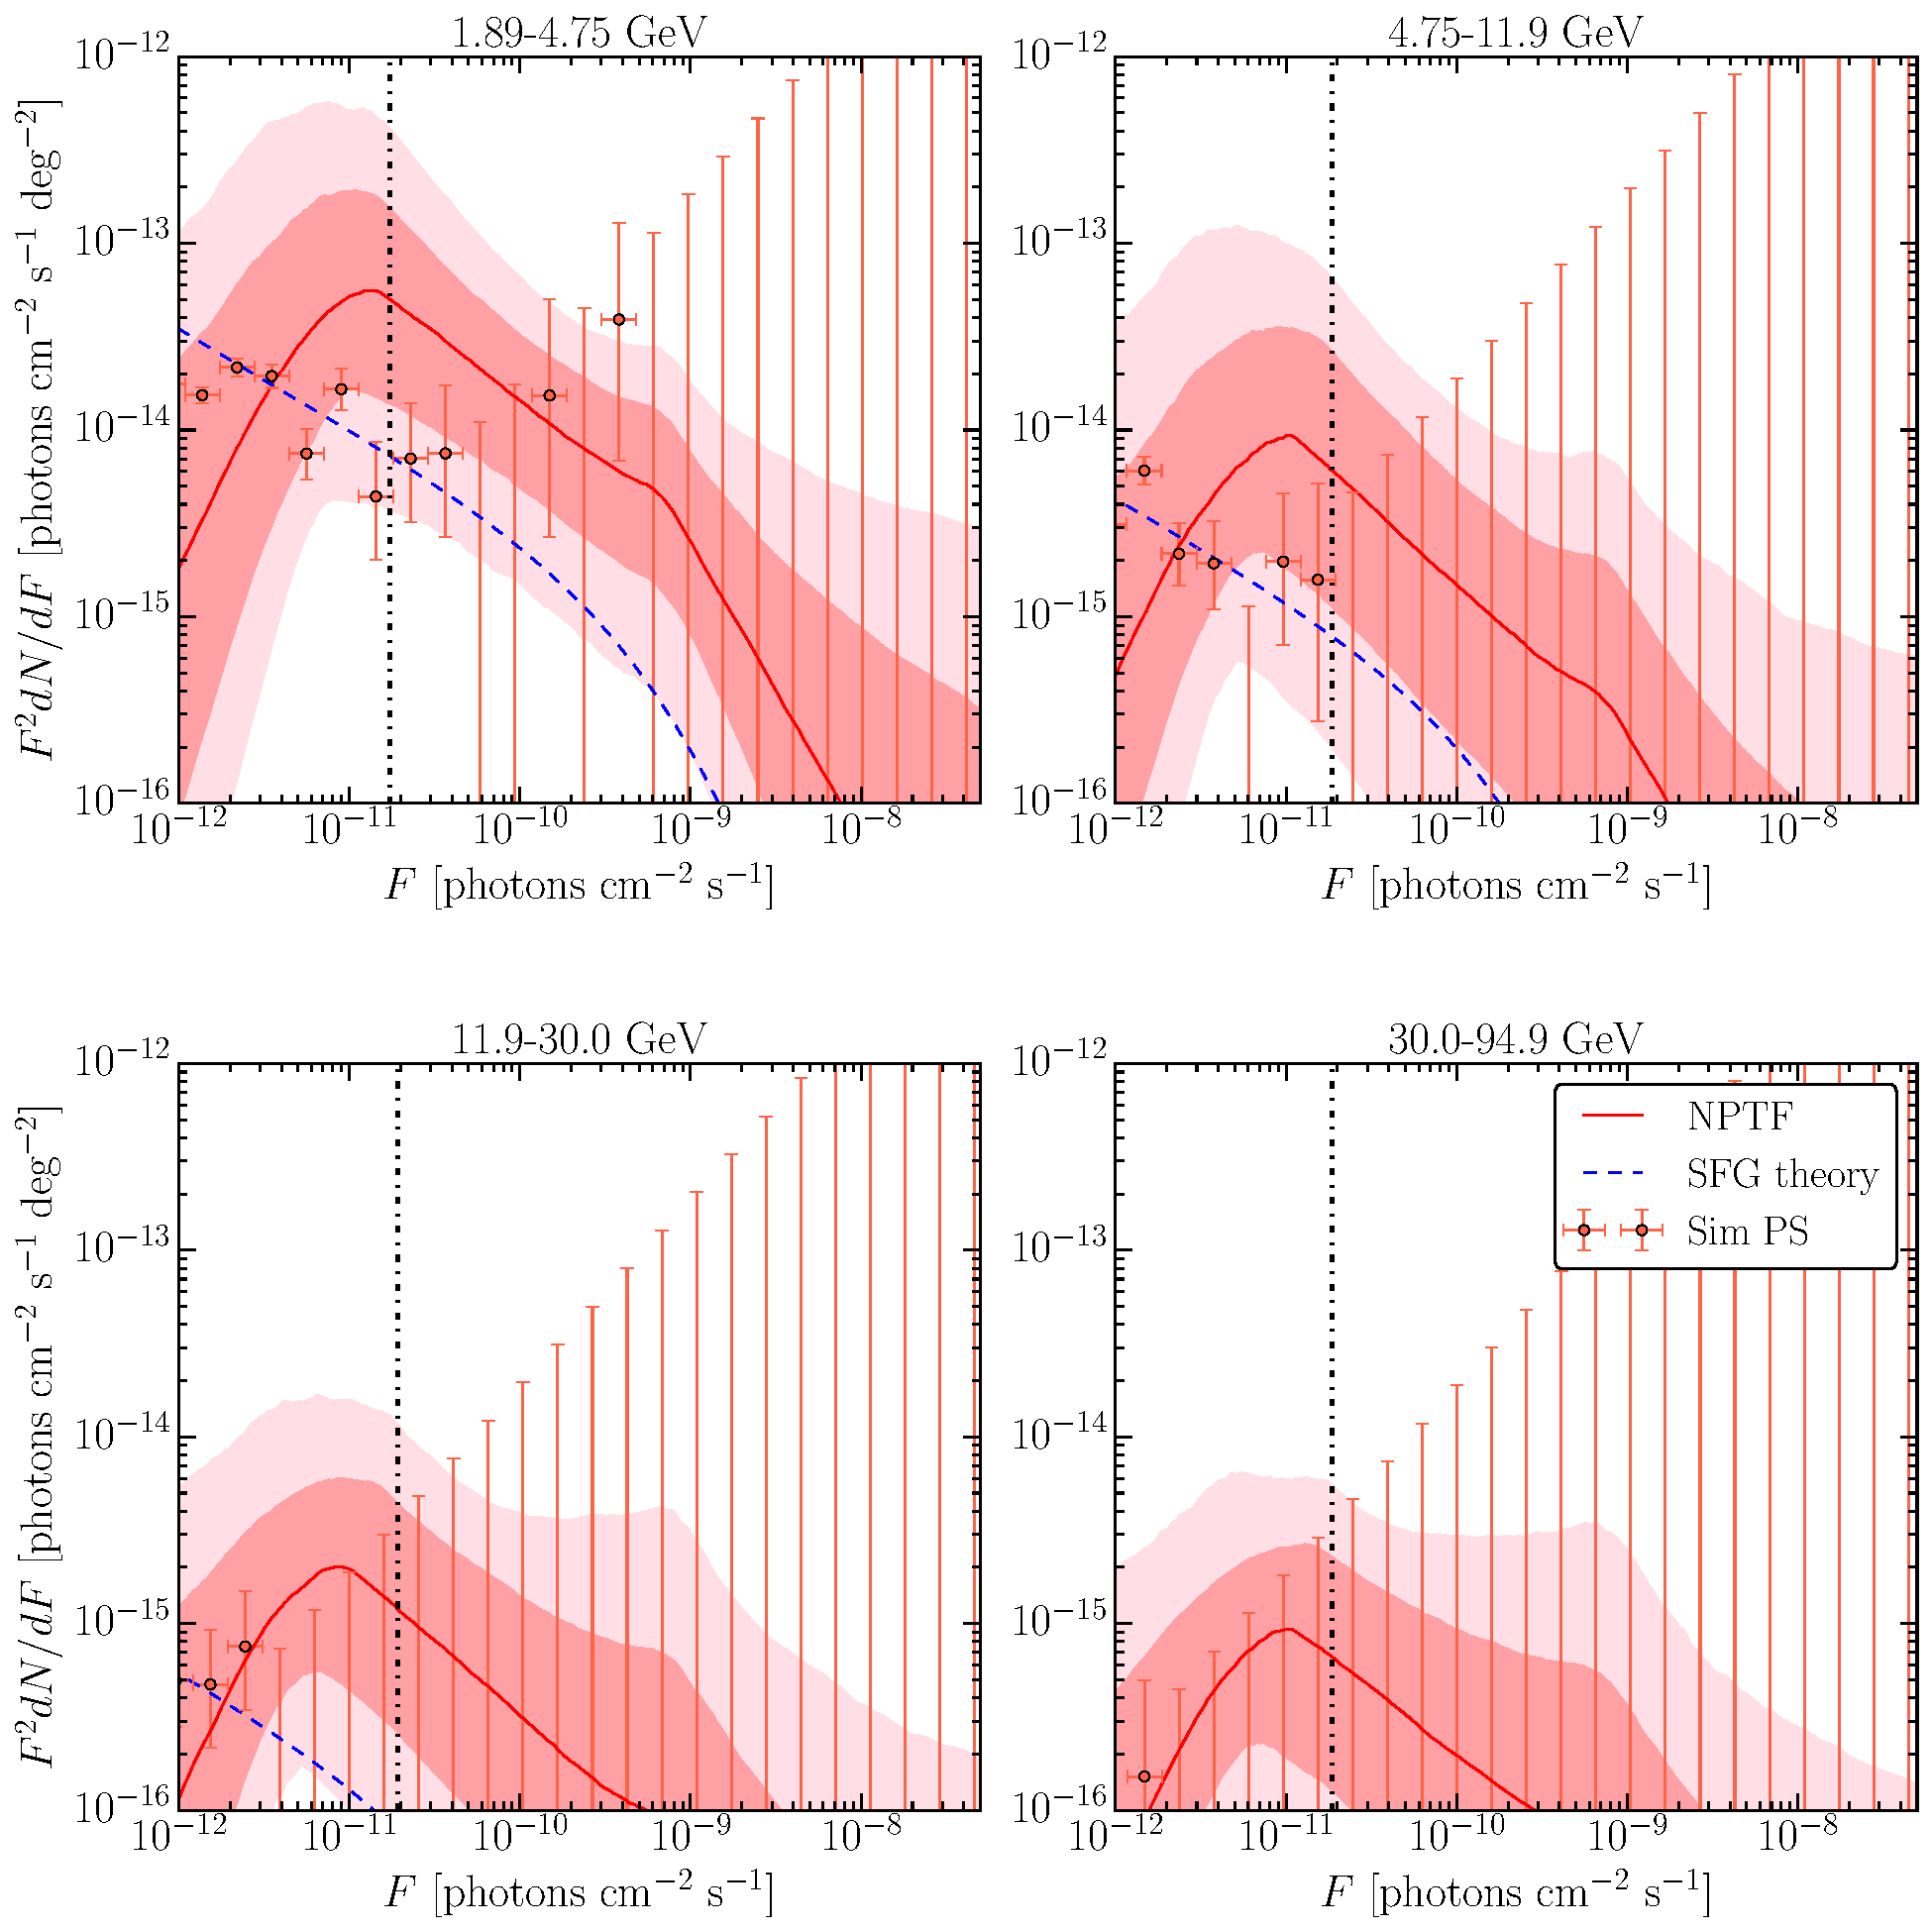
\includegraphics{ch-igrb/plots/sf-dnds.pdf}} 
		\end{array}$
	\end{center}
   \caption{Best-fit source-count distribution for a simulated map containing SFGs~\cite{Tamborra:2014xia}.  (Formatted as in Fig.~\ref{fig:bl1dnds}.) 
 }
   \label{fig:simdata_sfg} 
\end{figure}

\begin{figure}[htbp] %  figure placement: here, top, bottom, or page
   	\begin{center}$
	\begin{array}{c}
	\scalebox{0.5}{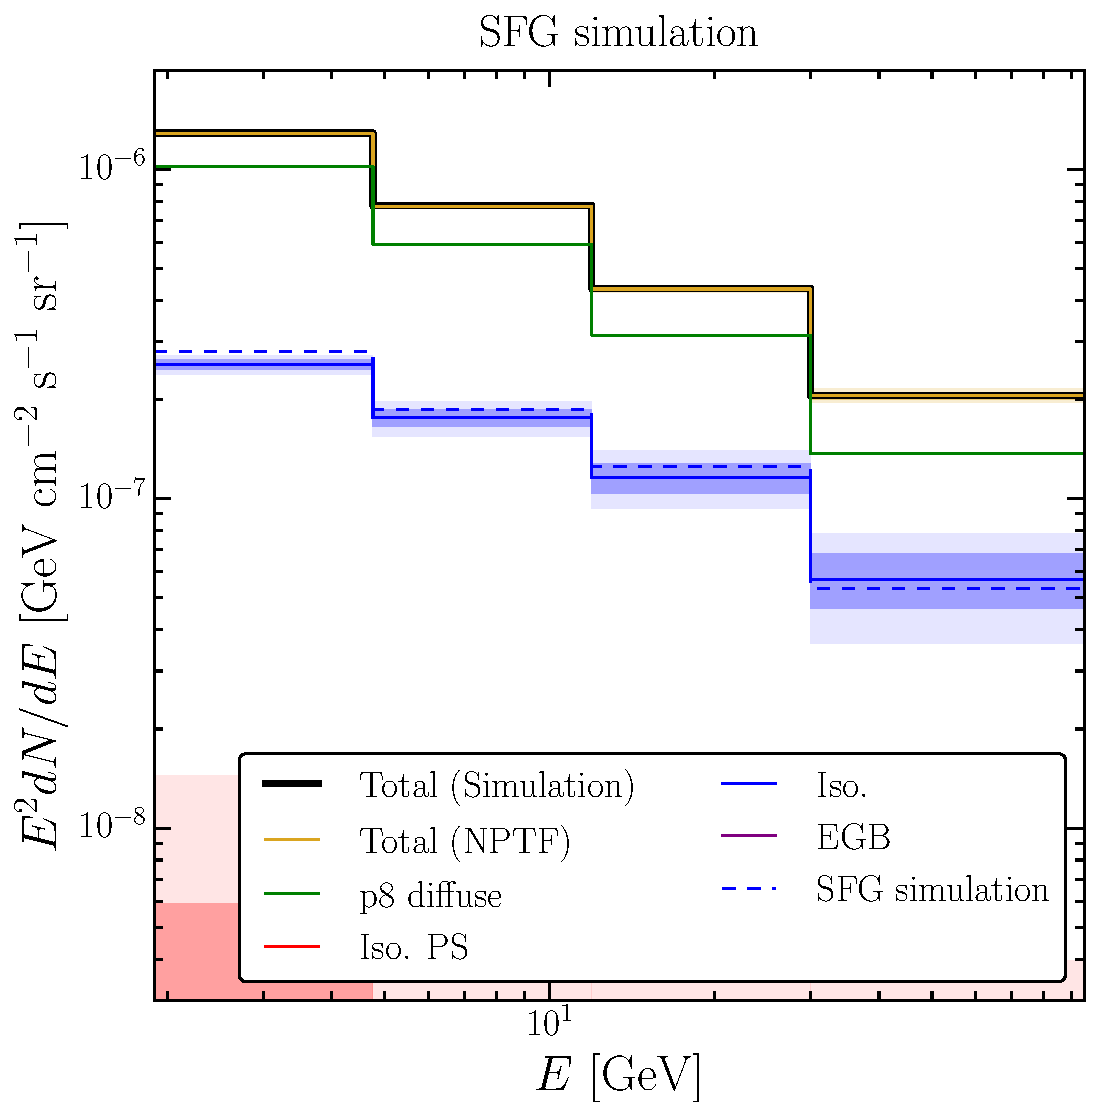
\includegraphics{ch-igrb/plots/sf-Espec.pdf}} 
		\end{array}$
	\end{center}
   \caption{Energy spectra for a simulated map containing SFGs~\cite{Tamborra:2014xia}.  (Formatted as in Fig.~\ref{fig:blESpec}.) }
   \label{fig:spec_sfg} 
\end{figure}

%\clearpage
%
%
\clearpage
\pagebreak


% \section{Supplementary Results: Low-Energy Analysis}

% \subsection{Best-Fit Intensities and Posterior Distributions}
% \label{app:suppanalysis_low}

% This section includes supplementary information pertaining to the low-energy analysis presented in Sec.~\ref{sec:benchmark}.  In particular, Tabs.~\ref{tab:bestfit_lowQ3} and~\ref{tab:bestfit_dndf_lowQ3} present the best-fit intensities and source-count parameters for the NPTF analysis of the top-three quartiles of {\it ultracleanveto} data.  Figures~\ref{fig:p8triangle1}--\ref{fig:p8triangle4} show the posterior distributions, in each energy bin, for the benchmark analysis.  
% \vspace{-1.5in}
% \begin{table}[phtb]
% \renewcommand{\arraystretch}{1.4}
% \setlength{\tabcolsep}{5pt}
% \begin{center}
% \begin{tabular}{ c  | c  c  c c  c   }
%  Energy & $I_\text{EGB}$&$I_\text{iso}^\text{PS}$ & $I_\text{iso}$ & $I_\text{diff}$ & $I_\text{bub}$   \\
% $[\text{GeV}]$ &  \multicolumn{5}{c}{$\left[\text{cm}^{-2}\text{ s}^{-1}\text{ sr}^{-1}\right]$}    \\
% \hline
% %\hline
% 1.89--4.75  
% &  $1.47_{-0.04}^{+0.05} \times 10^{-7}$ & $8.99_{-0.45}^{+0.53} \times 10^{-8}$ & $5.72_{-0.36}^{+0.30} \times 10^{-8}$ & $3.28_{-0.01}^{+0.01} \times 10^{-7}$ & $3.34_{-0.41}^{+0.39} \times 10^{-8}$\\
% % \hline
% 4.75--11.9 &    
% $5.60_{-0.17}^{+0.21} \times 10^{-8}$ & $2.85_{-0.18}^{+0.23} \times 10^{-8}$ & $2.74_{-0.16}^{+0.12} \times 10^{-8}$ & $7.69_{-0.08}^{+0.09} \times 10^{-8}$ & $1.52_{-0.23}^{+0.22} \times 10^{-8}$   \\
% % \hline
% 11.9--30.0  & 
% $1.85_{-0.07}^{+0.08} \times 10^{-8}$ & $8.54_{-0.71}^{+0.85} \times 10^{-9}$ & $9.92_{-0.63}^{+0.53} \times 10^{-9}$ & $1.68_{-0.04}^{+0.04} \times 10^{-8}$ & $5.59_{-1.31}^{+1.35} \times 10^{-9}$  \\  
% % \hline
% 30.0-94.9  &  
% $6.19_{-0.29}^{+0.42} \times 10^{-9}$ & $2.85_{-0.33}^{+0.39} \times 10^{-9}$ & $3.36_{-0.30}^{+0.25} \times 10^{-9}$ & $3.77_{-0.19}^{+0.17} \times 10^{-9}$ & $1.10_{-0.61}^{+0.72} \times 10^{-9}$  \\
% \end{tabular}
% \end{center}
% \caption{Same as Tab.~\ref{tab:bestfit}, except using the top three quartiles (PSF1--3) of the Pass~8 {\it ultracleanveto} data. }
% \label{tab:bestfit_lowQ3}
% \end{table}

% \vspace{-4in}
% \begin{table}[phtb]
% \renewcommand{\arraystretch}{1.4}
% \setlength{\tabcolsep}{3pt}
% \begin{center}
% \begin{tabular}{ c  | c  c  c c |  c c c   }
%  Energy & $n_1$ & $n_2$ & $n_3$ & $n_4$ & $F_{b,1}$ & $F_{b,2}$ & $F_{b,3}$   \\
% $[\text{GeV}]$ &  & & & & \multicolumn{3}{c}{$\left[\text{cm}^{-2}\text{ s}^{-1}\right]$}    \\
% \hline
% %\hline
% 1.89--4.75 &  
% $3.97_{-0.83}^{+0.69}$ & $2.10_{-0.03}^{+0.04}$ & $1.75_{-0.14}^{+0.09}$ & $-0.45_{-1.01}^{+1.10}$ & $8.16_{-3.00}^{+6.26} \times 10^{-9}$& $6.63_{-2.31}^{+3.45} \times 10^{-11}$ &$3.85_{-1.73}^{+1.38} \times 10^{-12}$     \\
% % \hline
% 4.75--11.9 &    
% $3.94_{-0.85}^{+0.68}$ & $2.08_{-0.05}^{+0.08}$ & $1.94_{-0.19}^{+0.07}$ & $-0.46_{-1.01}^{+1.07}$ & $3.85_{-1.65}^{+2.69} \times 10^{-9}$& $8.05_{-5.66}^{+7.34} \times 10^{-11}$ & $4.00_{-1.64}^{+1.36} \times 10^{-12}$    \\
% % \hline
% 11.9--30.0  & 
% $3.70_{-0.90}^{+0.82}$ & $2.20_{-0.14}^{+0.17}$ & $2.02_{-0.08}^{+0.07}$ & $-0.37_{-1.04}^{+1.05}$ & $2.69_{-1.34}^{+1.37} \times 10^{-9}$& $1.19_{-0.63}^{+0.45} \times 10^{-10}$ & $3.78_{-1.50}^{+1.33} \times 10^{-12}$ 
%   \\  
% % \hline
% 30.0-94.9  &  
% $3.54_{-0.90}^{+0.94}$ & $2.15_{-0.28}^{+0.24}$ & $2.21_{-0.11}^{+0.13}$ & $-0.09_{-1.20}^{+1.06}$ &  $1.59_{-0.73}^{+0.75} \times 10^{-9}$& $1.07_{-0.59}^{+0.49} \times 10^{-10}$ &  $3.37_{-1.48}^{+1.51} \times 10^{-12}$ \\
% \end{tabular}
% \end{center}
% \caption{Same as Tab.~\ref{tab:bestfit_dndf}, except using the top three quartiles (PSF1--3) of the Pass~8 {\it ultracleanveto} data.  }
% \label{tab:bestfit_dndf_lowQ3}
% \end{table}

% %\afterpage{%
% \begin{figure}[p] %  figure placement: here, top, bottom, or page
%    \centering
%    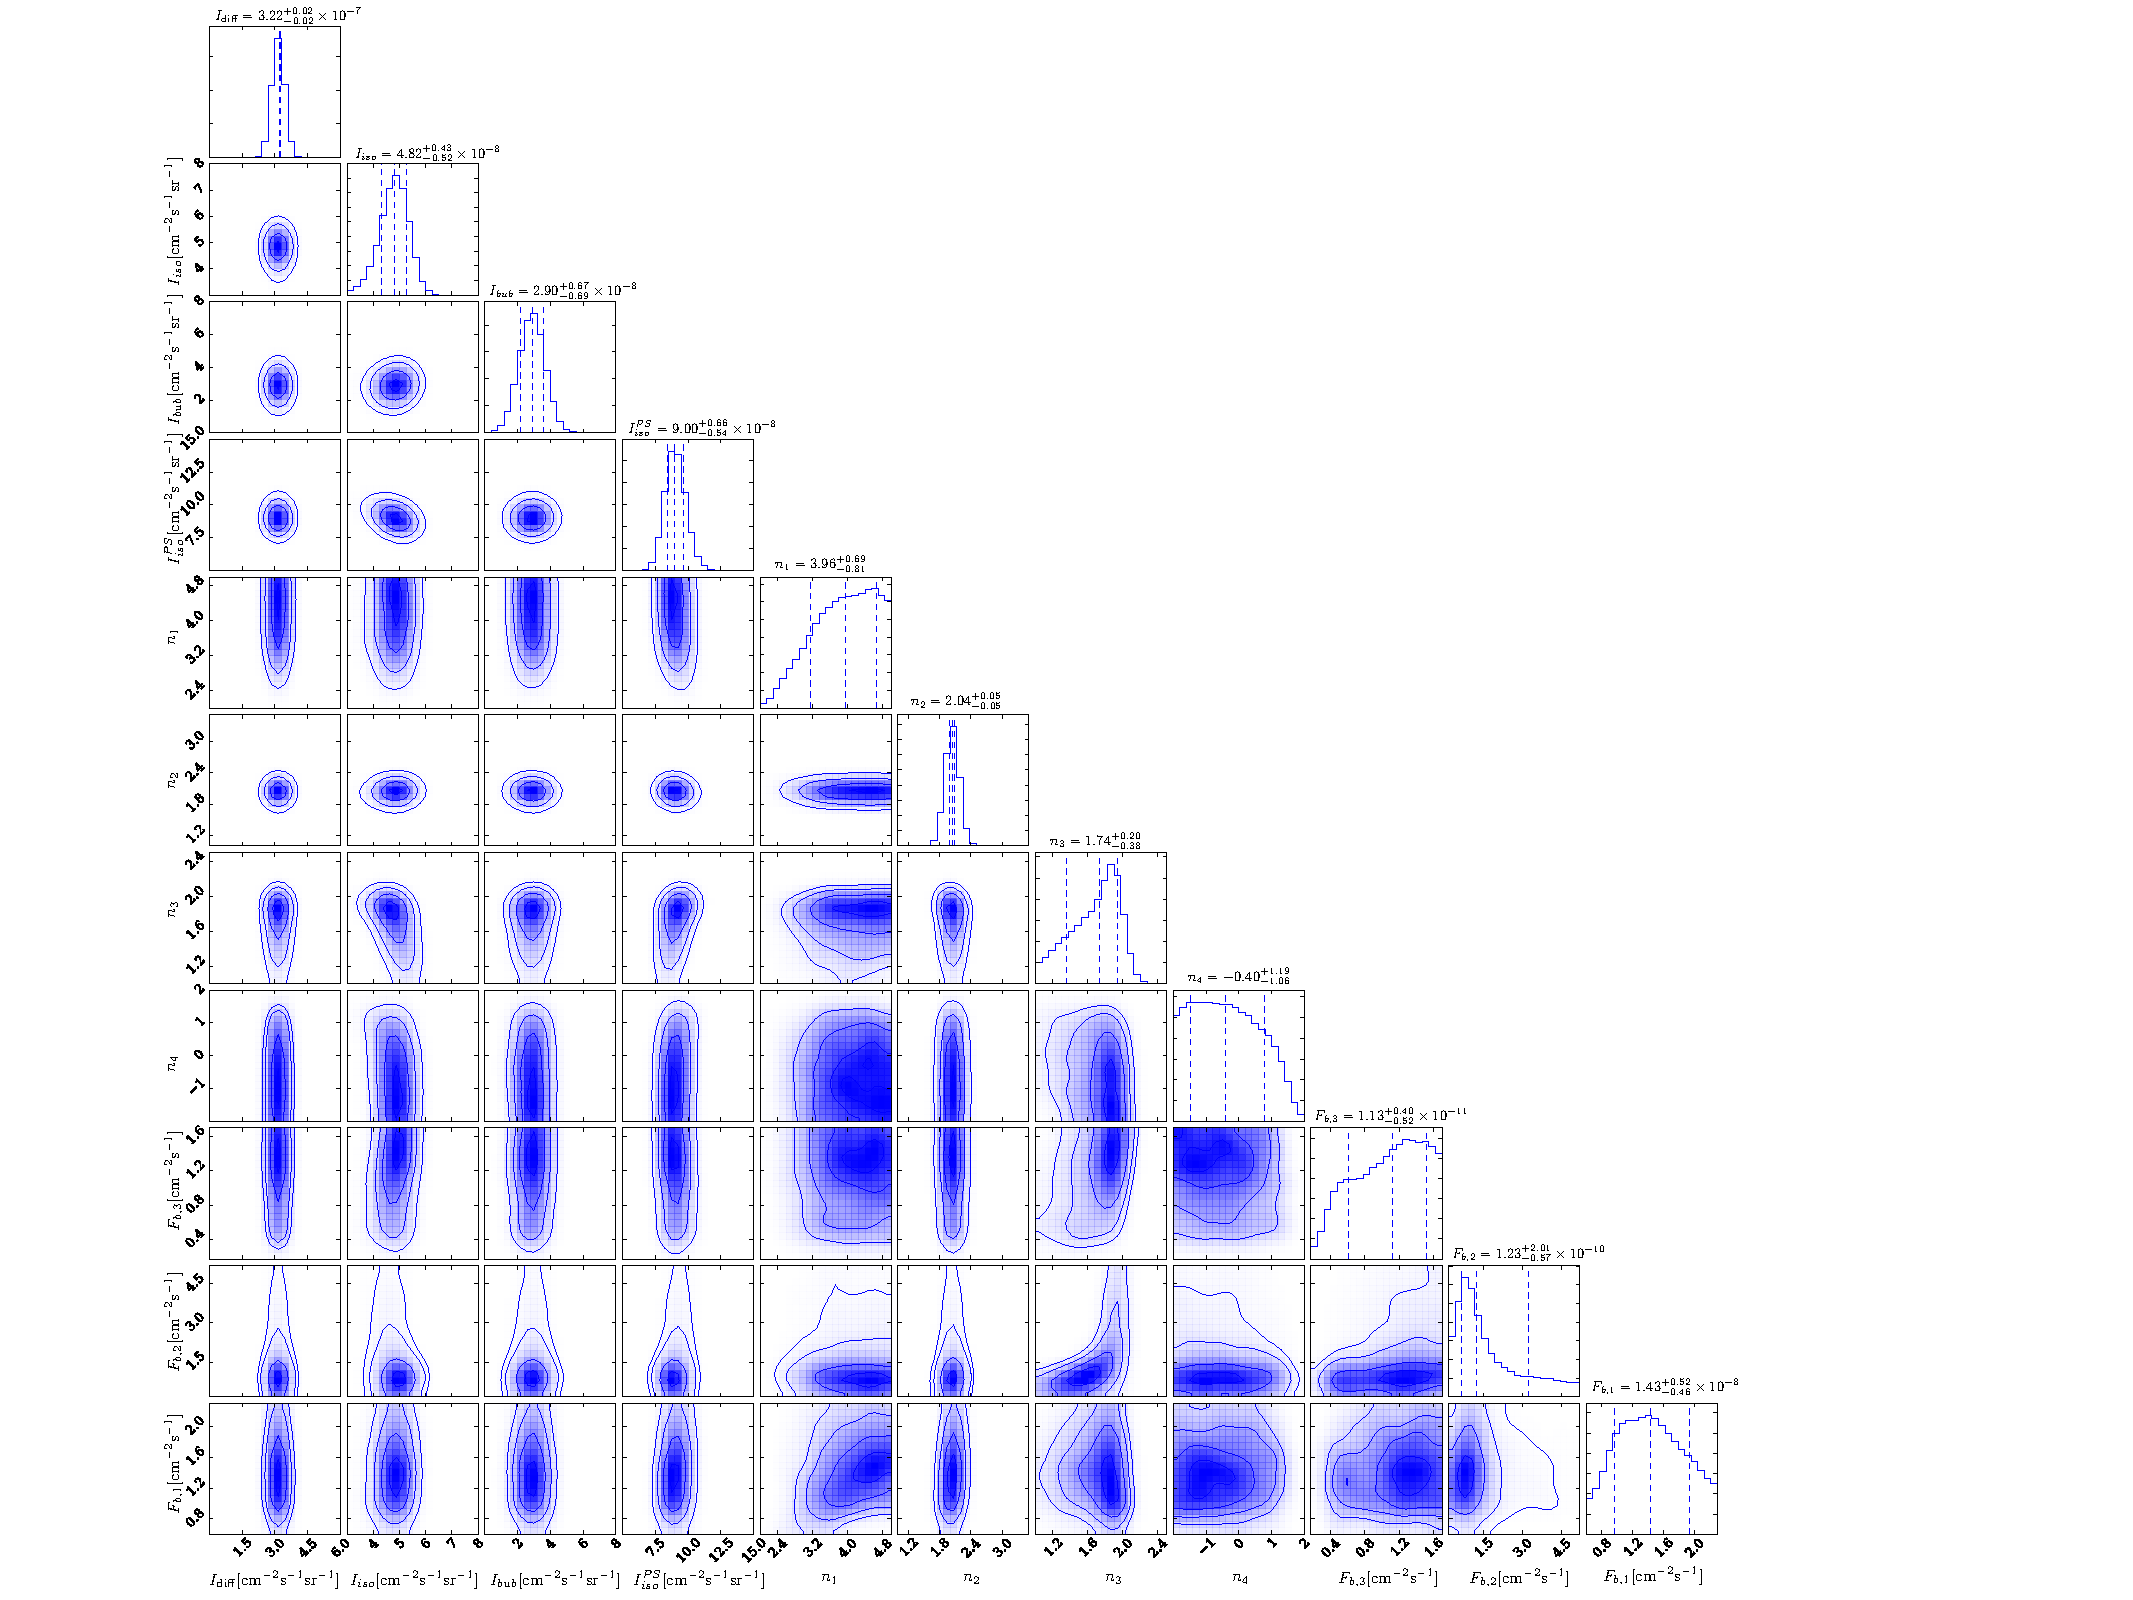
\includegraphics[trim={2cm 0 6cm 0},clip,width=\textwidth]{ch-igrb/plots/triangle_plot_8_12.pdf} 
%    \caption{Triangle plot for the 1.89--4.75~GeV bin.  The posterior distributions correspond to the NPTF analysis for Pass~8 {\it ultracleanveto} PSF3 data using the \texttt{p8r2} foreground model.  The \emph{Fermi} bubbles intensity is defined relative to the interior of the bubbles, while the intensities of the other templates are computed with respect to the region $\abs{b} \geq 30^\circ$. }  
%    \label{fig:p8triangle1} 
% \end{figure}
% %\clearpage
% %}

% \afterpage{%
% \begin{figure}[p] %  figure placement: here, top, bottom, or page
%    \centering
%    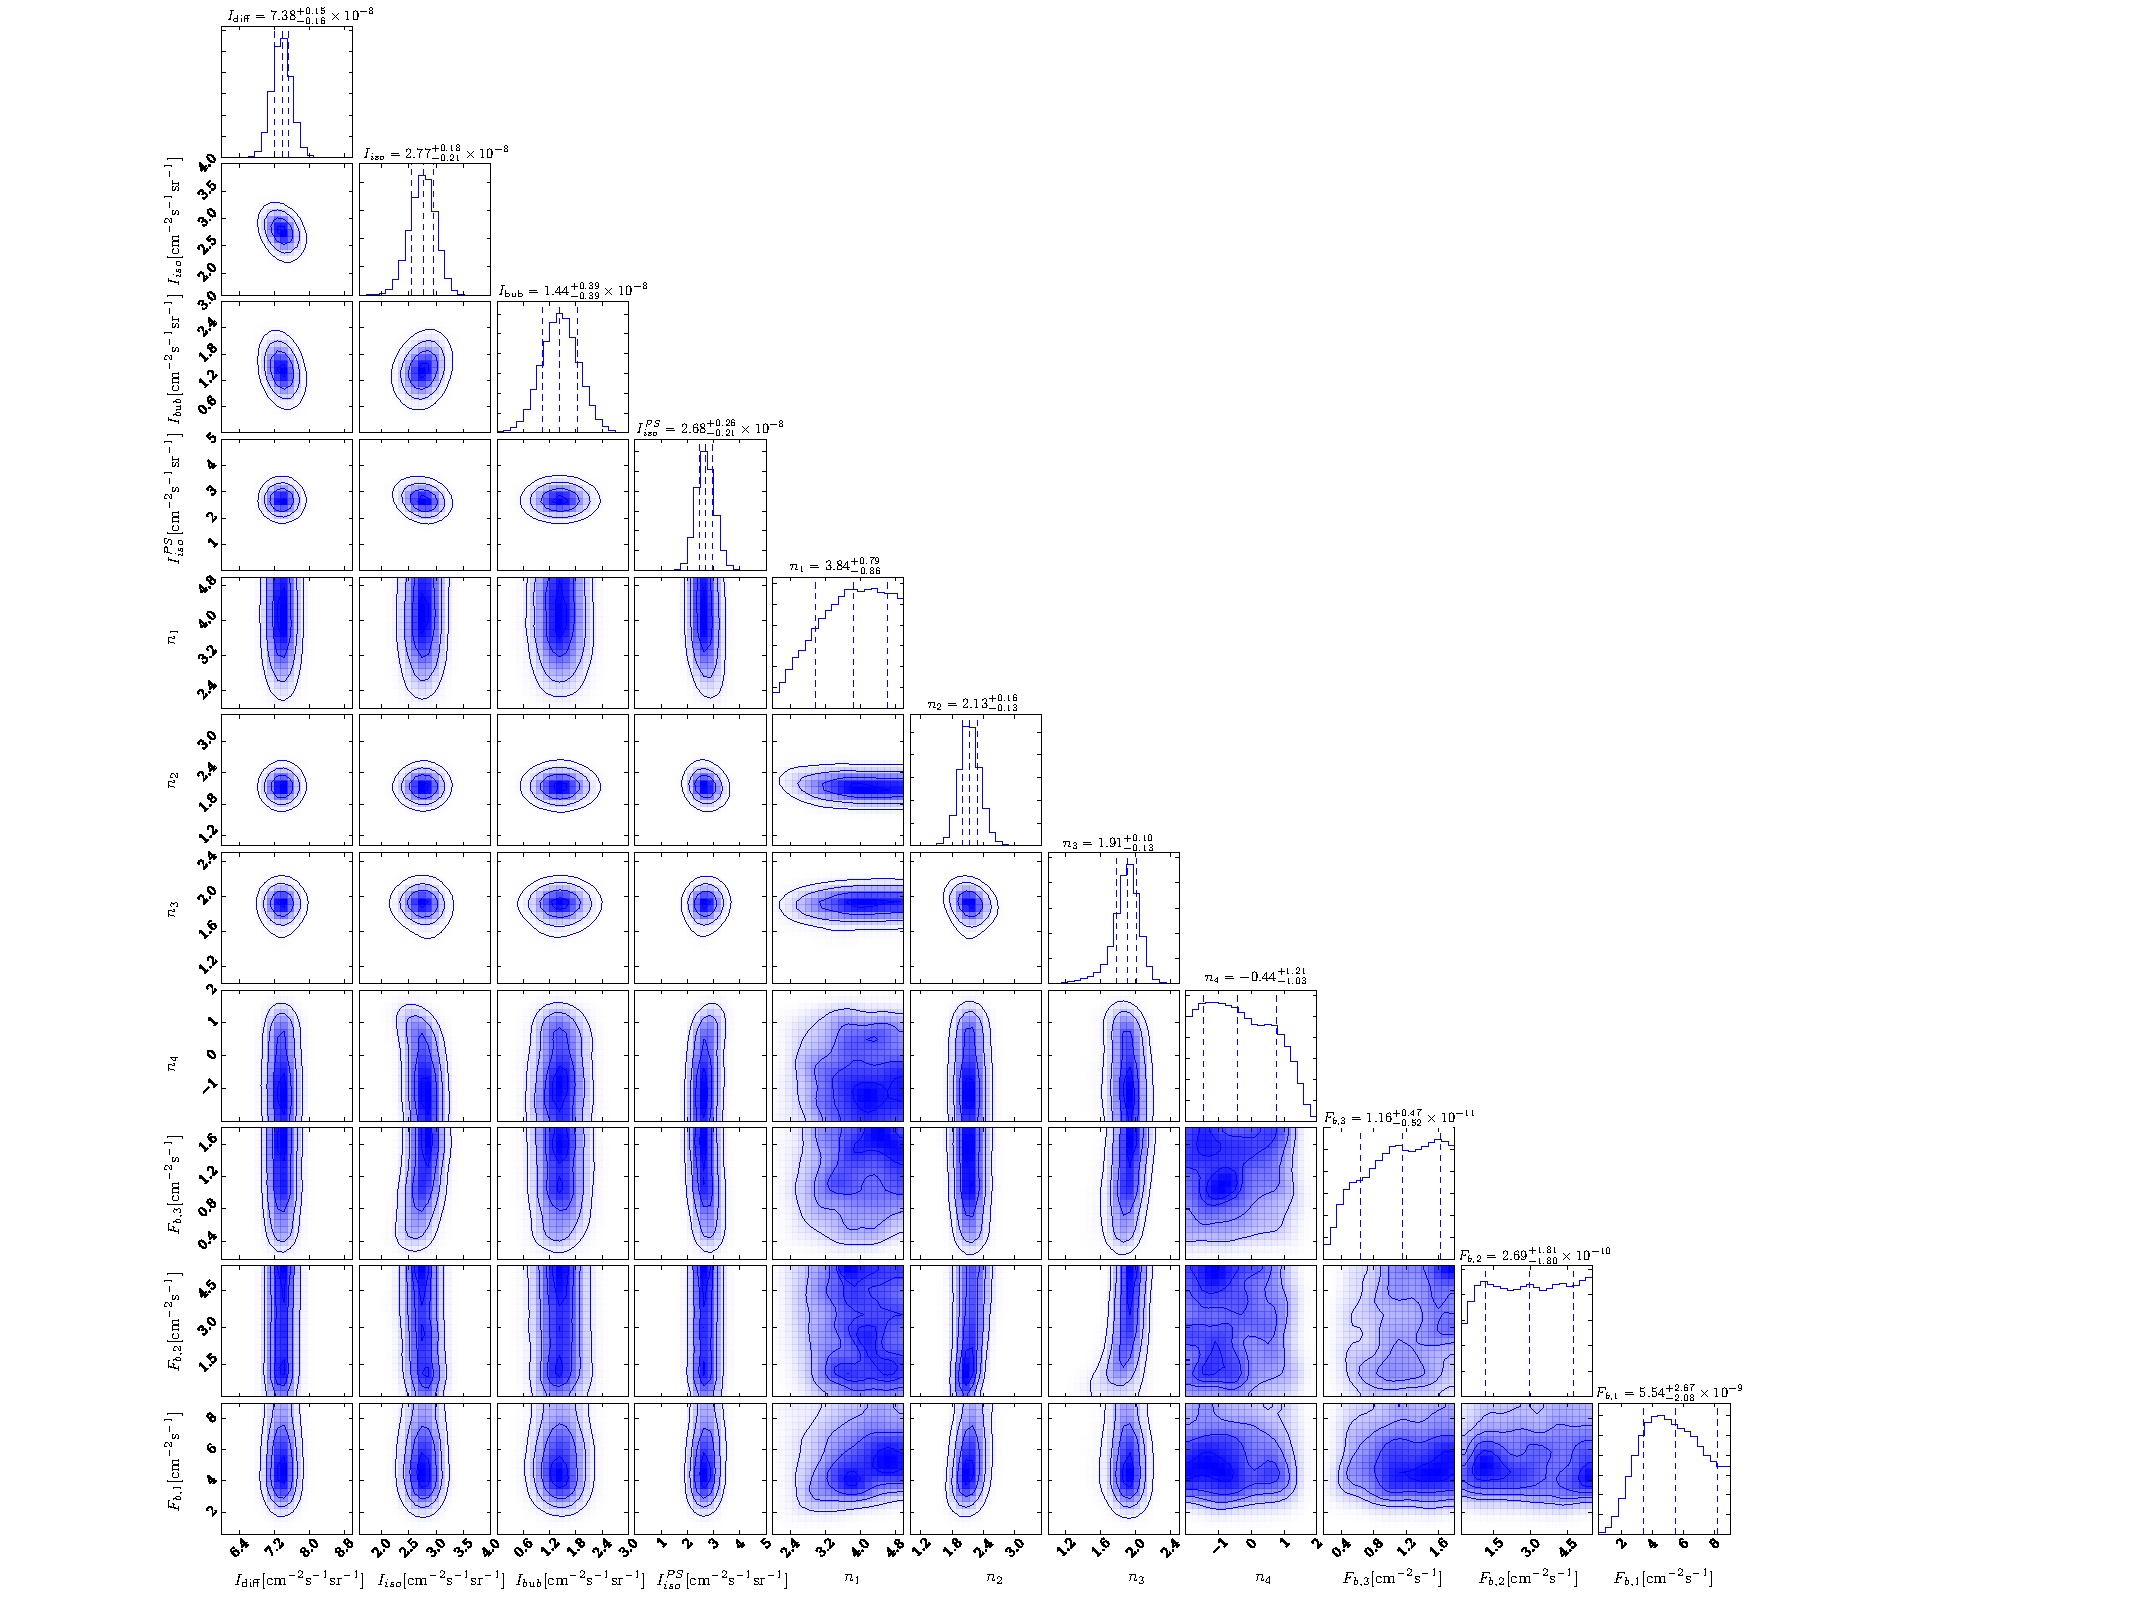
\includegraphics[trim={2cm 0 6cm 0},clip,width=\textwidth]{ch-igrb/plots/triangle_plot_12_16.pdf} 
%    \caption{Same as Fig.~\ref{fig:p8triangle1}, except for 4.75--11.9~GeV. }  
%    \label{fig:p8triangle2} 
% \end{figure}
% \clearpage
% }

% \afterpage{%
% \begin{figure}[tb] %  figure placement: here, top, bottom, or page
%    \centering
%    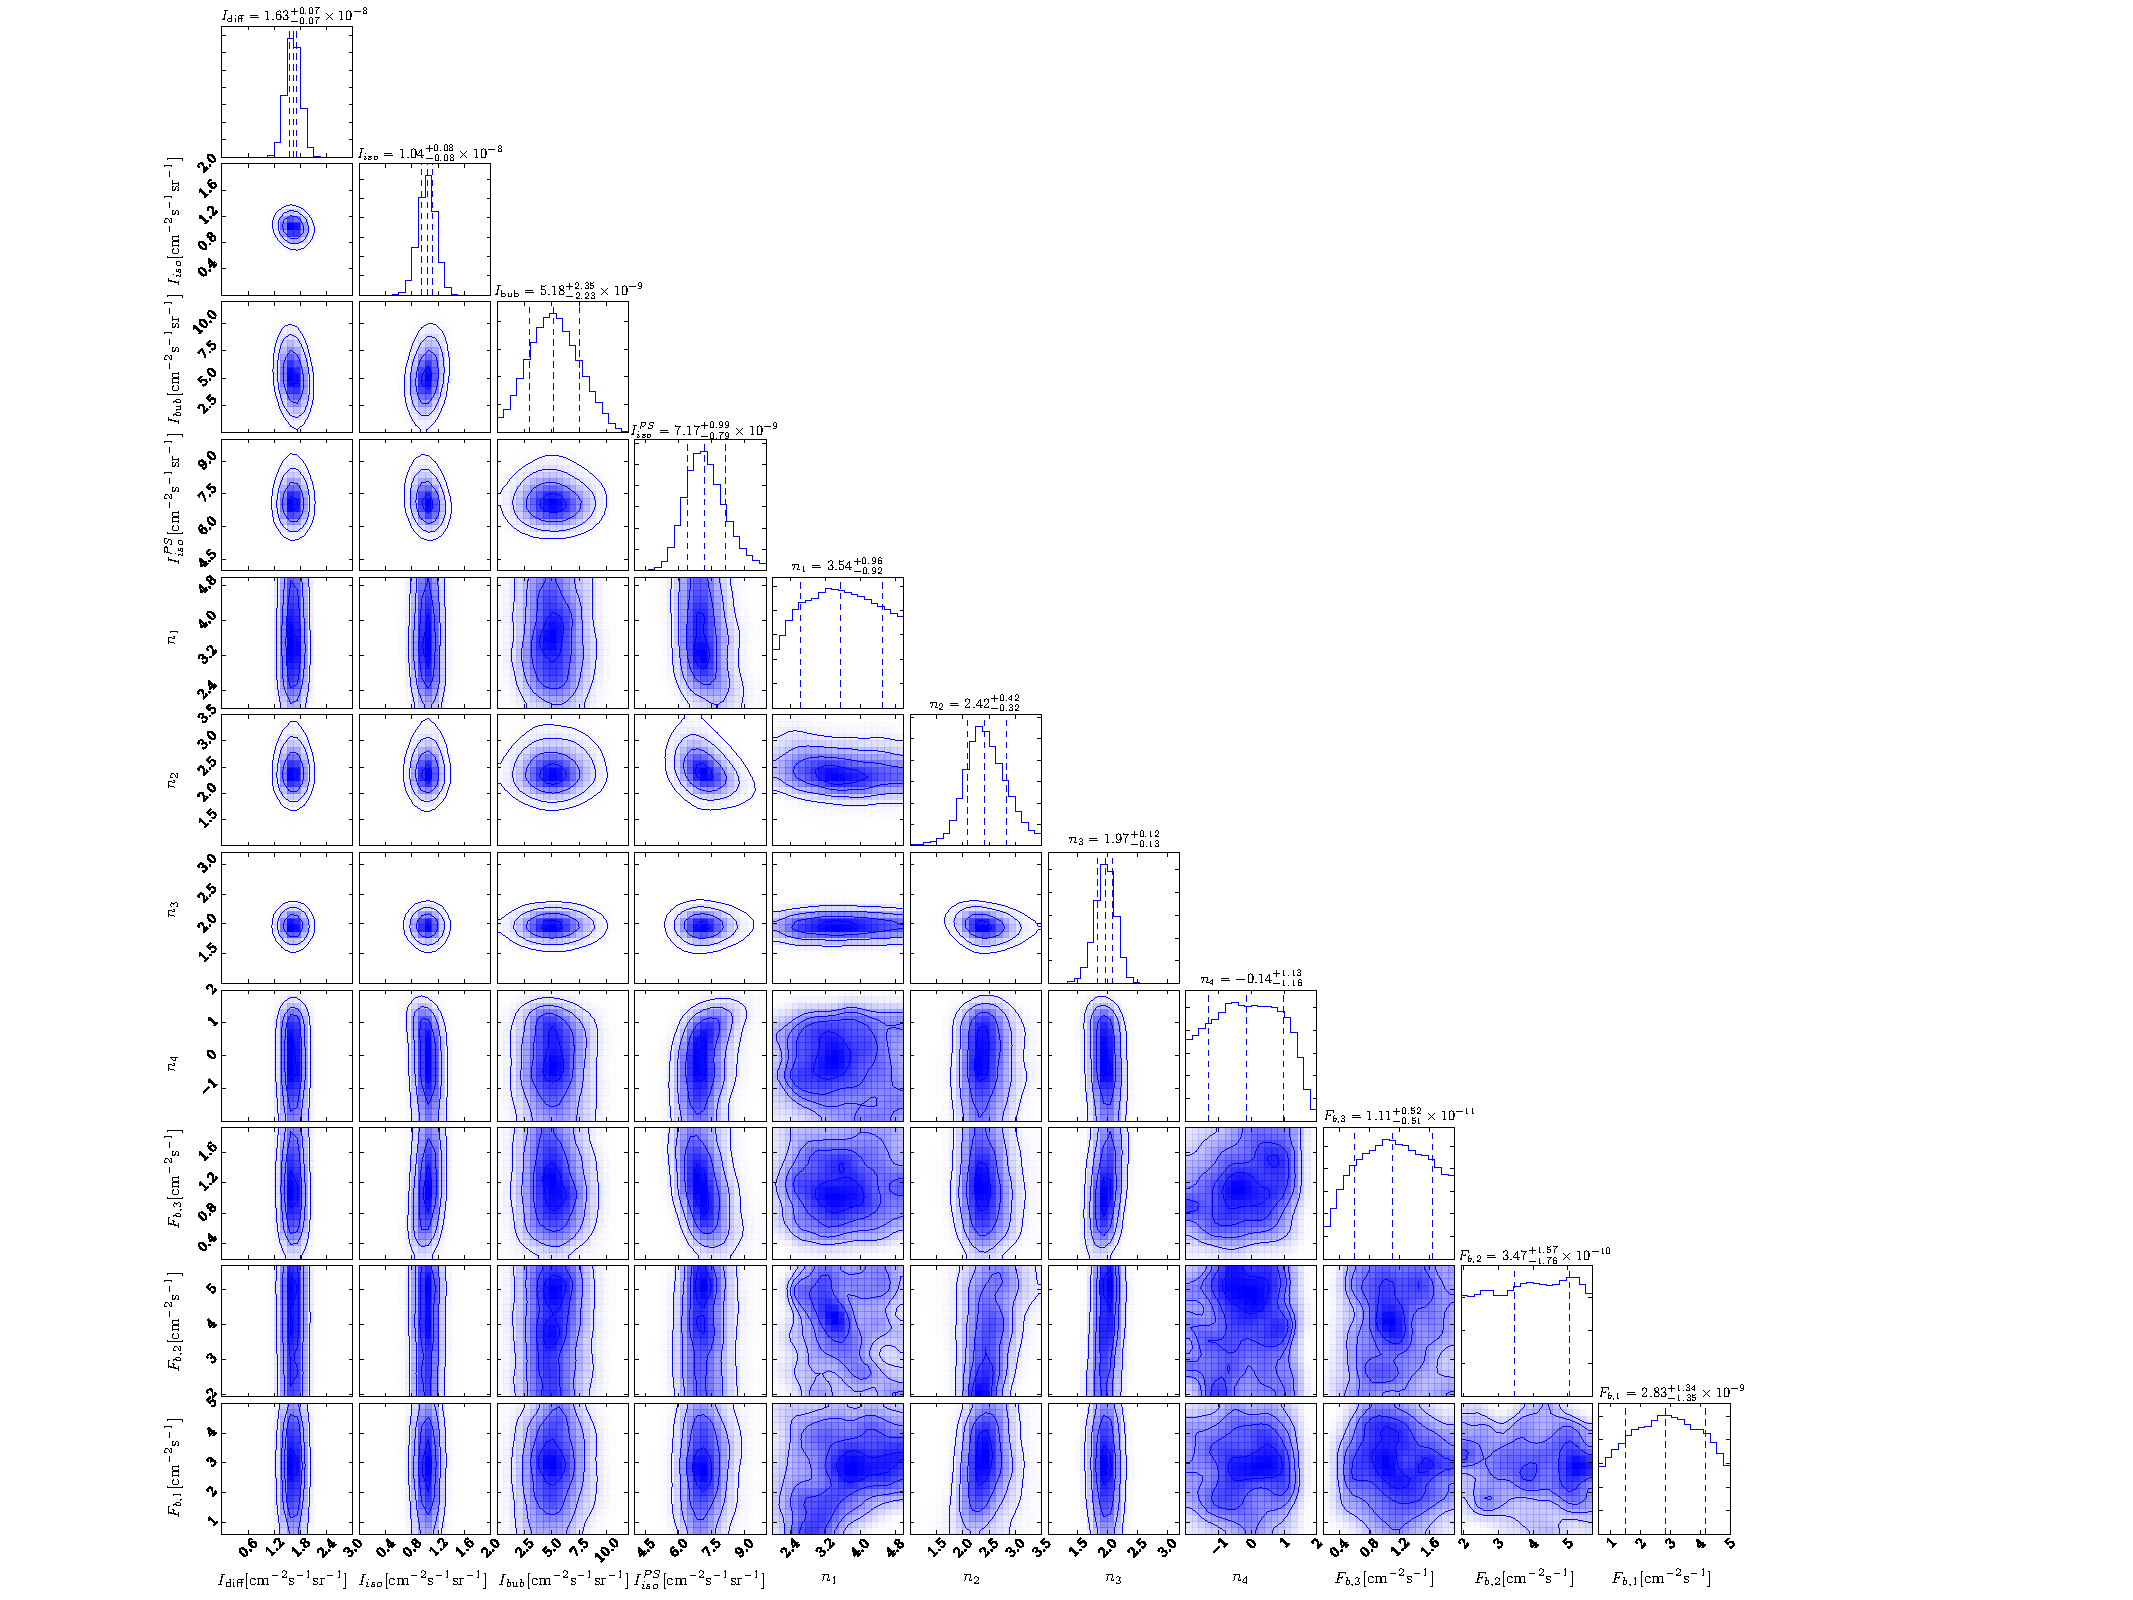
\includegraphics[trim={2cm 0 6cm 0},clip,width=\textwidth]{ch-igrb/plots/triangle_plot_16_20.pdf} 
%    \caption{Same as Fig.~\ref{fig:p8triangle1}, except for 11.9--30.0~GeV.}  
%    \label{fig:p8triangle3} 
% \end{figure}
% \clearpage
% }

% \afterpage{%
% \begin{figure}[tb] %  figure placement: here, top, bottom, or page
%    \centering
%    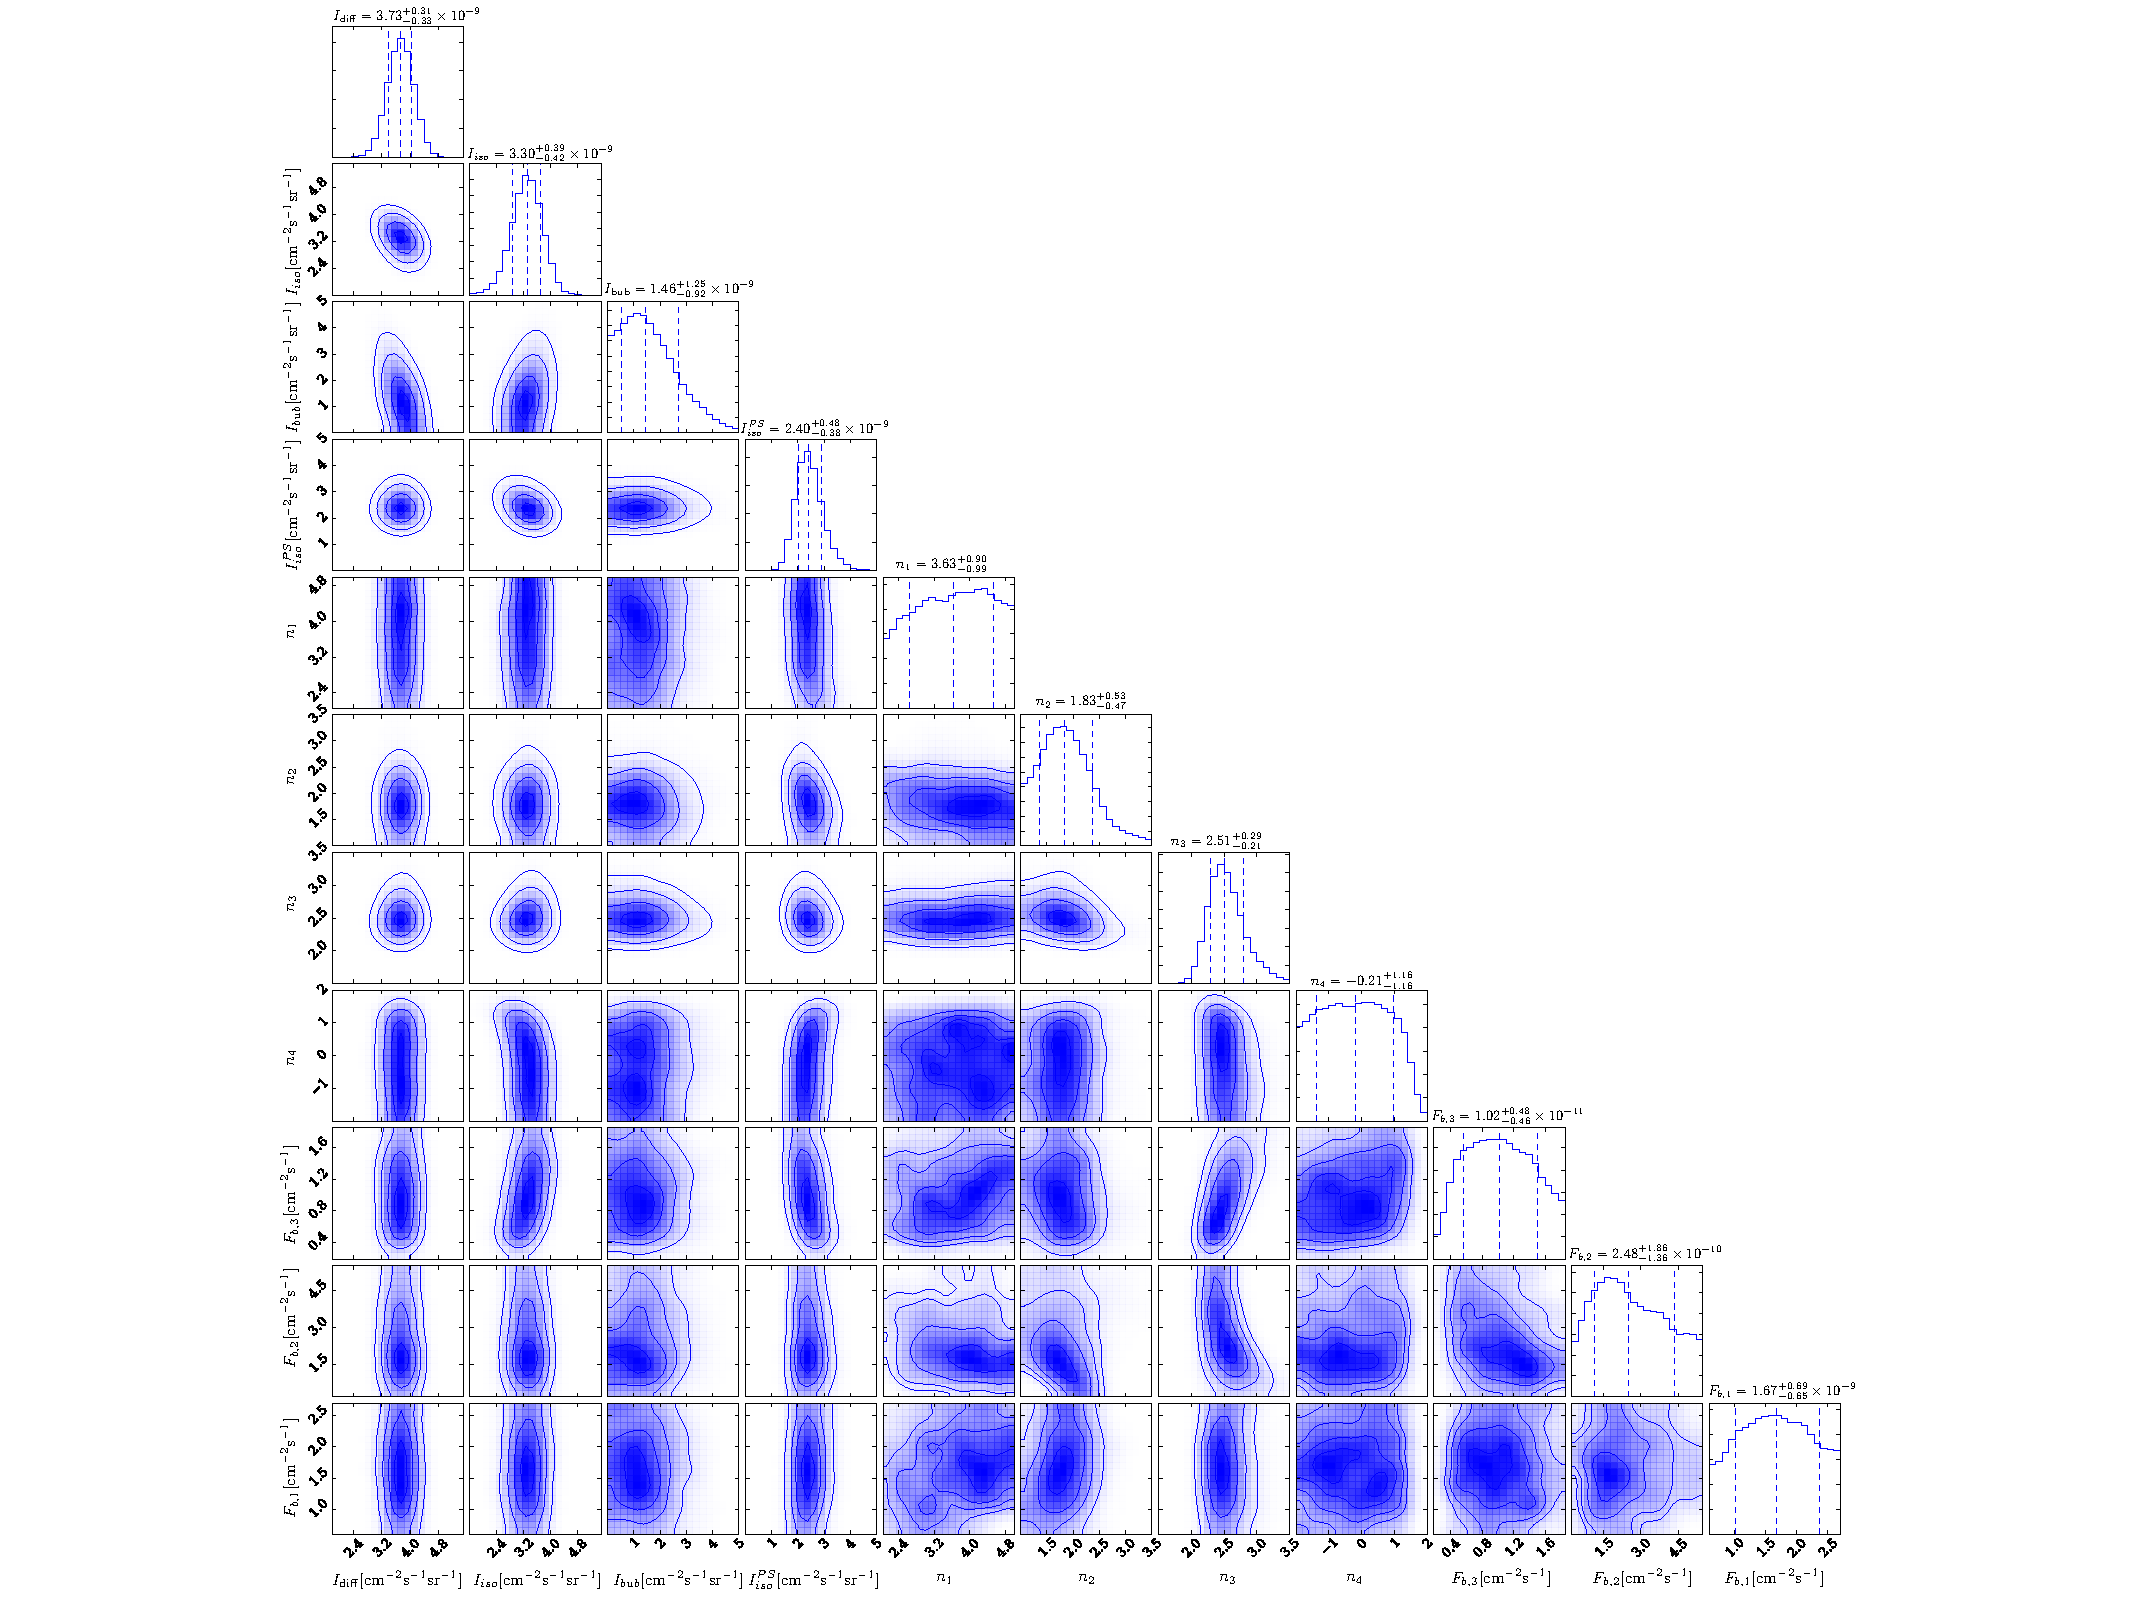
\includegraphics[trim={4cm 0 4cm 0},clip,width=\textwidth]{ch-igrb/plots/triangle_plot_20_25.pdf} 
%    \caption{Same as Fig.~\ref{fig:p8triangle1}, except for 30.0-94.9~GeV.}   
%    \label{fig:p8triangle4} 
% \end{figure}
% \clearpage
% }
% \pagebreak

% \subsection{Systematic Tests}
% \label{app:systematics}

% We now describe in detail the systematic tests that were conducted for the low-energy analysis, the results of which are summarized in Fig. \ref{fig:systematicsplot}.  The primary conclusion that we draw is that the the PS fraction is stable under the variety of tests that we have explored.  

% \subsubsection{Region of Interest}

% As a first cross-check on the stability of the results presented in Sec.~\ref{sec:benchmark}, we explore the effects of altering the region of interest.  While we previously defined the region of interest with $|b| \geq 30^\circ$, we now loosen this constraint and consider the case $|b| \geq 10^\circ$.  Extending the region of interest closer to the Galactic disk increases the amount of data being analyzed, but at the cost of potentially more contamination from diffuse foreground emission and local PSs.  As shown in Fig.~\ref{fig:systematicsplot}, the best-fit intensities for the isotropic and isotropic-PS components are equivalent, within errors, to their counterparts in the benchmark analysis. The best-fit source-counts are shown in Fig.~\ref{fig:dndsdata_m10}.

% We also ran the NPTF on the Northern ($b > 30^\circ$) and Southern ($b < -30^\circ$) hemispheres separately.  The intensities for the EGB, IGRB, and PS components are systematically lower (higher) for the Northern (Southern) analysis than for the benchmark case.  Similar behavior is apparent in the source-count plots, shown in Figs.~\ref{fig:dndsdata_north} and \ref{fig:dndsdata_south}.  



% \subsubsection{Event class}

% We explored the implications of broadening the {\it ultracleanveto} data set to include the top three quartiles in Sec. \ref{sec:benchmark_top3}.   Now, we consider the implications of repeating the NPTF analysis on the {\it source} data with PSF1--3.  This event class has looser photon-quality cuts, which leads to larger overall exposure, but significantly more cosmic-ray contamination.  In general, it is not recommended to use {\it source} data for IGRB studies; for our purposes, however, it will be intriguing to see how the increased photon statistics affect the recovered source-count distribution for the PS component.  As shown in Fig.~\ref{fig:systematicsplot}, the EGB intensity is far larger than that recovered by the benchmark analysis and overpredicts \emph{Fermi}'s EGB result in most energy bins.  The sharp rise in the EGB intensity can be traced to a substantial fraction of smooth isotropic emission, which is expected for this event class at most energies.  Most importantly, the intensity of the isotropic-PS component is consistent, within uncertainties, with that found in the benchmark analysis.\footnote{The recovered PS intensity is slightly larger with {\it source} PSF1--3 data as compared to {\it ultracleanveto} PSF3 data, which is likely due to the increased exposure in the {\it source} PSF1--3 data set. 
% }   This is a  confirmation that the NPTF is able to successfully constrain the source-count distribution even in a data set with significantly more smooth isotropic flux.  

% The source-count distributions are provided in Fig.~\ref{fig:dndsdata_source}.  In general, they exhibit similar behavior to the {\it ultracleanveto} PSF1--3 functions, extending to lower fluxes due to the increased exposure for this event class.  One potential new feature of interest in the {\it source}-data source-count distributions is that, in the second energy bin from $4.75$--$11.9$ GeV, there is a more pronounced hardening of the source-count distribution below the second break $F_{b,2}$, as compared to the {\it ultracleanveto} PSF1--3 analyses.

% \subsubsection{Foreground Model}
% \label{sec:foreground}

% A potentially significant source of systematic uncertainty in the NPTF analysis is due to mis-modeling of high-energy gamma-rays produced in cosmic-ray propagation in the Milky Way~\cite{Ackermann:2012pya}.  These high-energy photons arise from  bremsstrahlung of electrons off the interstellar medium, boosted pion decay, and inverse Compton (IC)  emission off the interstellar radiation field.  Our benchmark analysis uses 
% the associated foreground model for the Pass~8 data set (\emph{gll\_iem\_v06.fits}), denoted here as \texttt{p8r2}.  The total diffuse emission in \texttt{p8r2} is modeled as a linear combination of several sources, some of which are traced by maps of gas column densities, which serve as templates for the pion and bremsstrahlung emission.  The IC component is modeled using the \texttt{GALPROP} package~\cite{Strong:2007nh}.\footnote{\url{http://galprop.stanford.edu/}}  These individual templates are fit to the data, and used to identify `extended emission excesses' that are identified directly and then added back into the model~\cite{Acero-2016}.

% To better assess the uncertainties due to the foreground modeling, we repeat the NPTF analysis using several other foreground models made available by \emph{Fermi}.  In particular, we use the \emph{gll\_iem\_v02\_P6\_V11\_DIFFUSE.fits} diffuse emission model, denoted as \texttt{p6v11}, which was initially developed for the Pass~6 data set.\footnote{\url{http://fermi.gsfc.nasa.gov/ssc/data/access/lat/ring_for_FSSC_final4.pdf}}  \texttt{p6v11} is distinct from \texttt{p8r2} in that it uses older gas and IC maps and does not include templates for large-scale structure or extended emission excesses.  The Pass~7 model \emph{gal\_2yearp7v6\_v0.fits}, denoted as \texttt{p7v6},\footnote{\url{http://fermi.gsfc.nasa.gov/ssc/data/access/lat/Model_details/Pass7_galactic.html}} is a compromise as it uses updated gas and IC maps and includes some large-scale extended structures, such as Loop~1 and the \emph{Fermi} bubbles.

% The NPTF results using the \texttt{p6v11} and \texttt{p7v6} foreground models are summarized in Fig.~\ref{fig:systematicsplot}, with source-count distributions  shown in Figs.~\ref{fig:dndsdata_p6} and~\ref{fig:dndsdata_p7}, respectively. In general, we observe that the intensity of the PS components is consistent with that for the benchmark analysis in all energy bins.  However, variations occur in the smooth isotropic intensity.  Typically, more IGRB intensity is recovered with \texttt{p6v11} and \texttt{p7v6}, versus \texttt{p8r2}.  The differences are particularly dramatic in the first two energy bins and are more severe for \texttt{p6v11}.  The net consequence is that the EGB intensity is higher than the expected range from \emph{Fermi}.  The enhancement in the isotropic component may arise from the fact that each foreground model incorporates large-scale diffuse structures differently---with \texttt{p6v11} being the least inclusive and \texttt{p8r2} being the most inclusive.  We note, however, that the fit to data with the \texttt{p8r2} foreground model, from the point of view of the Bayesian evidence, is much better than the analogous fit with the  \texttt{p6v11} model; the fit with the \texttt{p7v6} model is intermediate. 

% \subsubsection{The Bubbles Template}

% To better understand how dependent the analysis is on the details of the \emph{Fermi} bubbles template, we simply removed the template from the analysis.  This has indiscernible effects on the final results.  We see in Fig.~\ref{fig:systematicsplot} that the EGB, IGRB, and PS intensities are consistent, within uncertainties, to the corresponding values in the benchmark study.  The source-count distributions, shown in Fig.~\ref{fig:dndsdata_nobub}, are also degenerate with those found including the \emph{Fermi} bubbles template.   

% \subsubsection{Point Spread Function}

% The PSF can affect the photon-count distribution because it can redistribute photons between pixels, and must therefore be properly accounted for in the calculation of the photon-count probability distributions.  For the primary analyses presented in this work, the PSF is modeled using a King function.  However, to test the sensitivity of the results to mis-modeling of the PSF, we have also repeated the NPTF analysis using a two-dimensional Gaussian in the calculation of the photon-count probability distributions, with a width set to give the correct 68\% containment radius.  As shown in Fig.~\ref{fig:systematicsplot}, the NPTF results remain unchanged with this substitution.  The best-fit source-count distribution for 1.89--4.75~GeV shows some variation at the lowest fluxes, but within uncertainties (see Fig.~\ref{fig:dndsdata_gauss}).    

% \subsubsection{Priors}

% Our choice of priors, given in Tab.~\ref{tab:priors}, is carefully chosen to both avoid biasing the posterior for the source-count distribution while at the same time allowing breaks at both high and low flux.  This is meant to properly account for the fact that the source-count distribution is not well constrained by the data at very high fluxes, where the mean expected number of sources over the full region is much less than unity, and at very low fluxes, where the mean photon-count per source is much less than unity.  Our choice of priors is further justified by the simulated data studies, presented in Sec.~\ref{sec:simulations}, which show that the NPTF can successfully constrain the emission from blazar models.  However, one may still be concerned that these particular choice of priors might bias the recovered source-count distribution in a particular way.  For that reason, we have tried many variations to the priors shown in Tab.~\ref{tab:priors}, three of which (labeled `alternate priors 1--3')  are described below and shown in Fig.~\ref{fig:systematicsplot}:
% \begin{itemize}
% \item {\it Alternate prior 1}:  All priors are the same as in Tab.~\ref{tab:priors}, except for those on the breaks, which are changed to $[0.1,10]$, $[10,40]$, and $[40, 2 \times S_\text{b,max}]$ ph for $S_{b,1}$, $S_{b,2}$, and $S_{b,3}$, respectively. 
% \item {\it Alternate prior 2}:  As above, except changing the priors for the breaks to $[1,20]$, $[20,S_\text{b,max}/2]$, and $[S_\text{b,max}/2, 2 \times S_\text{b,max}]$ ph, respectively.
% \item {\it Alternate prior 3}:  All priors are the same as in Tab.~\ref{tab:priors}, except for that of $n_4$, which is changed to $[1,1.99]$.
% \end{itemize}

% The first two examples address the possibility that the break priors might artificially sculpt the source-count distribution and the recovered PS intensity, while the third example addresses how the source-count distribution is dealt with at fluxes below the lowest break, where the distribution is not well constrained by the data.  In many classes of blazar models, such as those considered in Sec.~\ref{sec:simulations}, the index below the lowest break ($n_4$) is greater than unity, so that the total number of PSs $\sim$$\int_{F_\text{min}} dF \, dN / dF$ diverges as the minimum flux cut-off $F_\text{min}$ is taken to zero.

% It is useful to know if the recovered PS intensity, $I_\text{iso}^\text{PS}$, tends to under or overshoot the simulated blazar intensity, $I_\text{blazar-sim}$, when using the alternate priors.  With that in mind, we run the NPTF on simulated maps, as in Sec.~\ref{sec:simulations}, constructed from both the SFG + Blazar--1 model as well as the SFG + Blazar--2 model.   For \emph{Alternate prior 1}, we find that
% \begin{equation}
% {I_\text{iso}^\text{PS} \over I_\text{blazar-sim}} = [0.87_{-0.04}^{+0.05},0.93_{-0.08}^{+0.17},0.92_{-0.15}^{+0.23},0.61_{-0.07}^{+0.11}]  \nonumber
% \end{equation}
% and
% \begin{equation}
% {I_\text{iso}^\text{PS} \over I_\text{blazar-sim}} = [0.68_{-0.05}^{+0.06},0.59_{-0.09}^{+0.15},0.52_{-0.05}^{+0.07},0.37_{-0.03}^{+0.05}]  \nonumber
% \end{equation} 
% for the SFG + Blazar--1 and SFG + Blazar--2 models, respectively, with {\it ultracleanveto} PSF3 instrument response function.
% With {\it Alternate prior 1}, we see larger uncertainties, with the PS template capable of absorbing more flux in particular.  With \emph{Alternate prior 2}, on the other hand, we find more noticeable differences in the medians as well as in the uncertainties.  In particular, for the SFG + Blazar--1 and SFG + Blazar--2 models, we find
% \begin{equation}
% {I_\text{iso}^\text{PS} \over I_\text{blazar-sim}} = [1.01_{-0.10}^{+0.12}, 1.27_{-0.31}^{+0.16}, 1.25_{-0.15}^{+0.12}, 0.73_{-0.12}^{+0.21}]  \nonumber
% \end{equation}
% and
% \begin{equation}
% {I_\text{iso}^\text{PS} \over I_\text{blazar-sim} }= [0.74_{-0.06}^{+0.19}, 0.94_{-0.19}^{+0.20}, 0.61_{-0.10}^{+0.17}, 0.41_{-0.05}^{+0.09}] \,, \nonumber
% \end{equation} 
% respectively.  In the Blazar--1 model case, it is important to notice that at intermediate energies the NPTF tends to over-predict $I_\text{blazar-sim}$ at the $\sim$20\% level.  With \emph{Alternate prior 3}, the results are 
% \begin{equation}
% {I_\text{iso}^\text{PS} \over I_\text{blazar-sim}} = [1.06_{-0.09}^{+0.15}, 1.10_{-0.09}^{+0.14}, 1.00_{-0.10}^{+0.14}, 0.85_{-0.11}^{+0.15}]  \nonumber
% \end{equation}
% and
% \begin{equation}
% {I_\text{iso}^\text{PS} \over I_\text{blazar-sim}} = [0.92_{-0.09}^{+0.16}, 0.77_{-0.14}^{+0.39}, 0.69_{-0.08}^{+0.12}, 0.53_{-0.06}^{+0.10}] \,, \nonumber
% \end{equation} 
% for the Blazar--1 and Blazar--2 models.  The \emph{Alternate prior 3} results are consistently closer to unity than the first two alternate prior results. 

% As may be seen in Fig.~\ref{fig:systematicsplot}, the median values for the PS intensities recovered from the NPTF analyses with alternate priors are generally consistent with those found in the baseline study.  The {\it Alternate prior 3} PS intensities are slightly enhanced in all energy bins compared to the baseline results---following our expectations from the simulation results presented above---though the two results are consistent within statistical uncertainties.  The recovered source-count distributions, shown in Fig.~\ref{fig:dndsdata_altpriors3}, illustrate that the {\it Alternate prior 3} results are consistent with our baseline results at fluxes above the $\sim$1 photon threshold.  At lower fluxes, the source-count distributions are slightly softer than in our baseline analysis, as is almost guaranteed by that fact that $n_4 > 1$ with {\it Alternate prior 3} while $n_4 > -2$ in our baseline analysis.   

% The {\it Alternate prior 1} and {\it Alternate prior 2} results have mean PS intensities similar to those in the baseline analysis, though in the second and third energy bin the upper limits of the credible intervals extend to higher values.  This is a reflection of the fact that the recovered source-count distributions, shown in Figs.~\ref{fig:dndsdata_altpriors1}, \ref{fig:dndsdata_altpriors2}, are softer at low fluxes compared to those in the baseline analysis.  This is perhaps due to the fact that the lowest break tends to be at higher flux, and thus the index $n_4$ is influenced by the data in the vicinity of the break.  

% \afterpage{
% \begin{figure*}[phtb] %  figure placement: here, top, bottom, or page
%    \centering
%    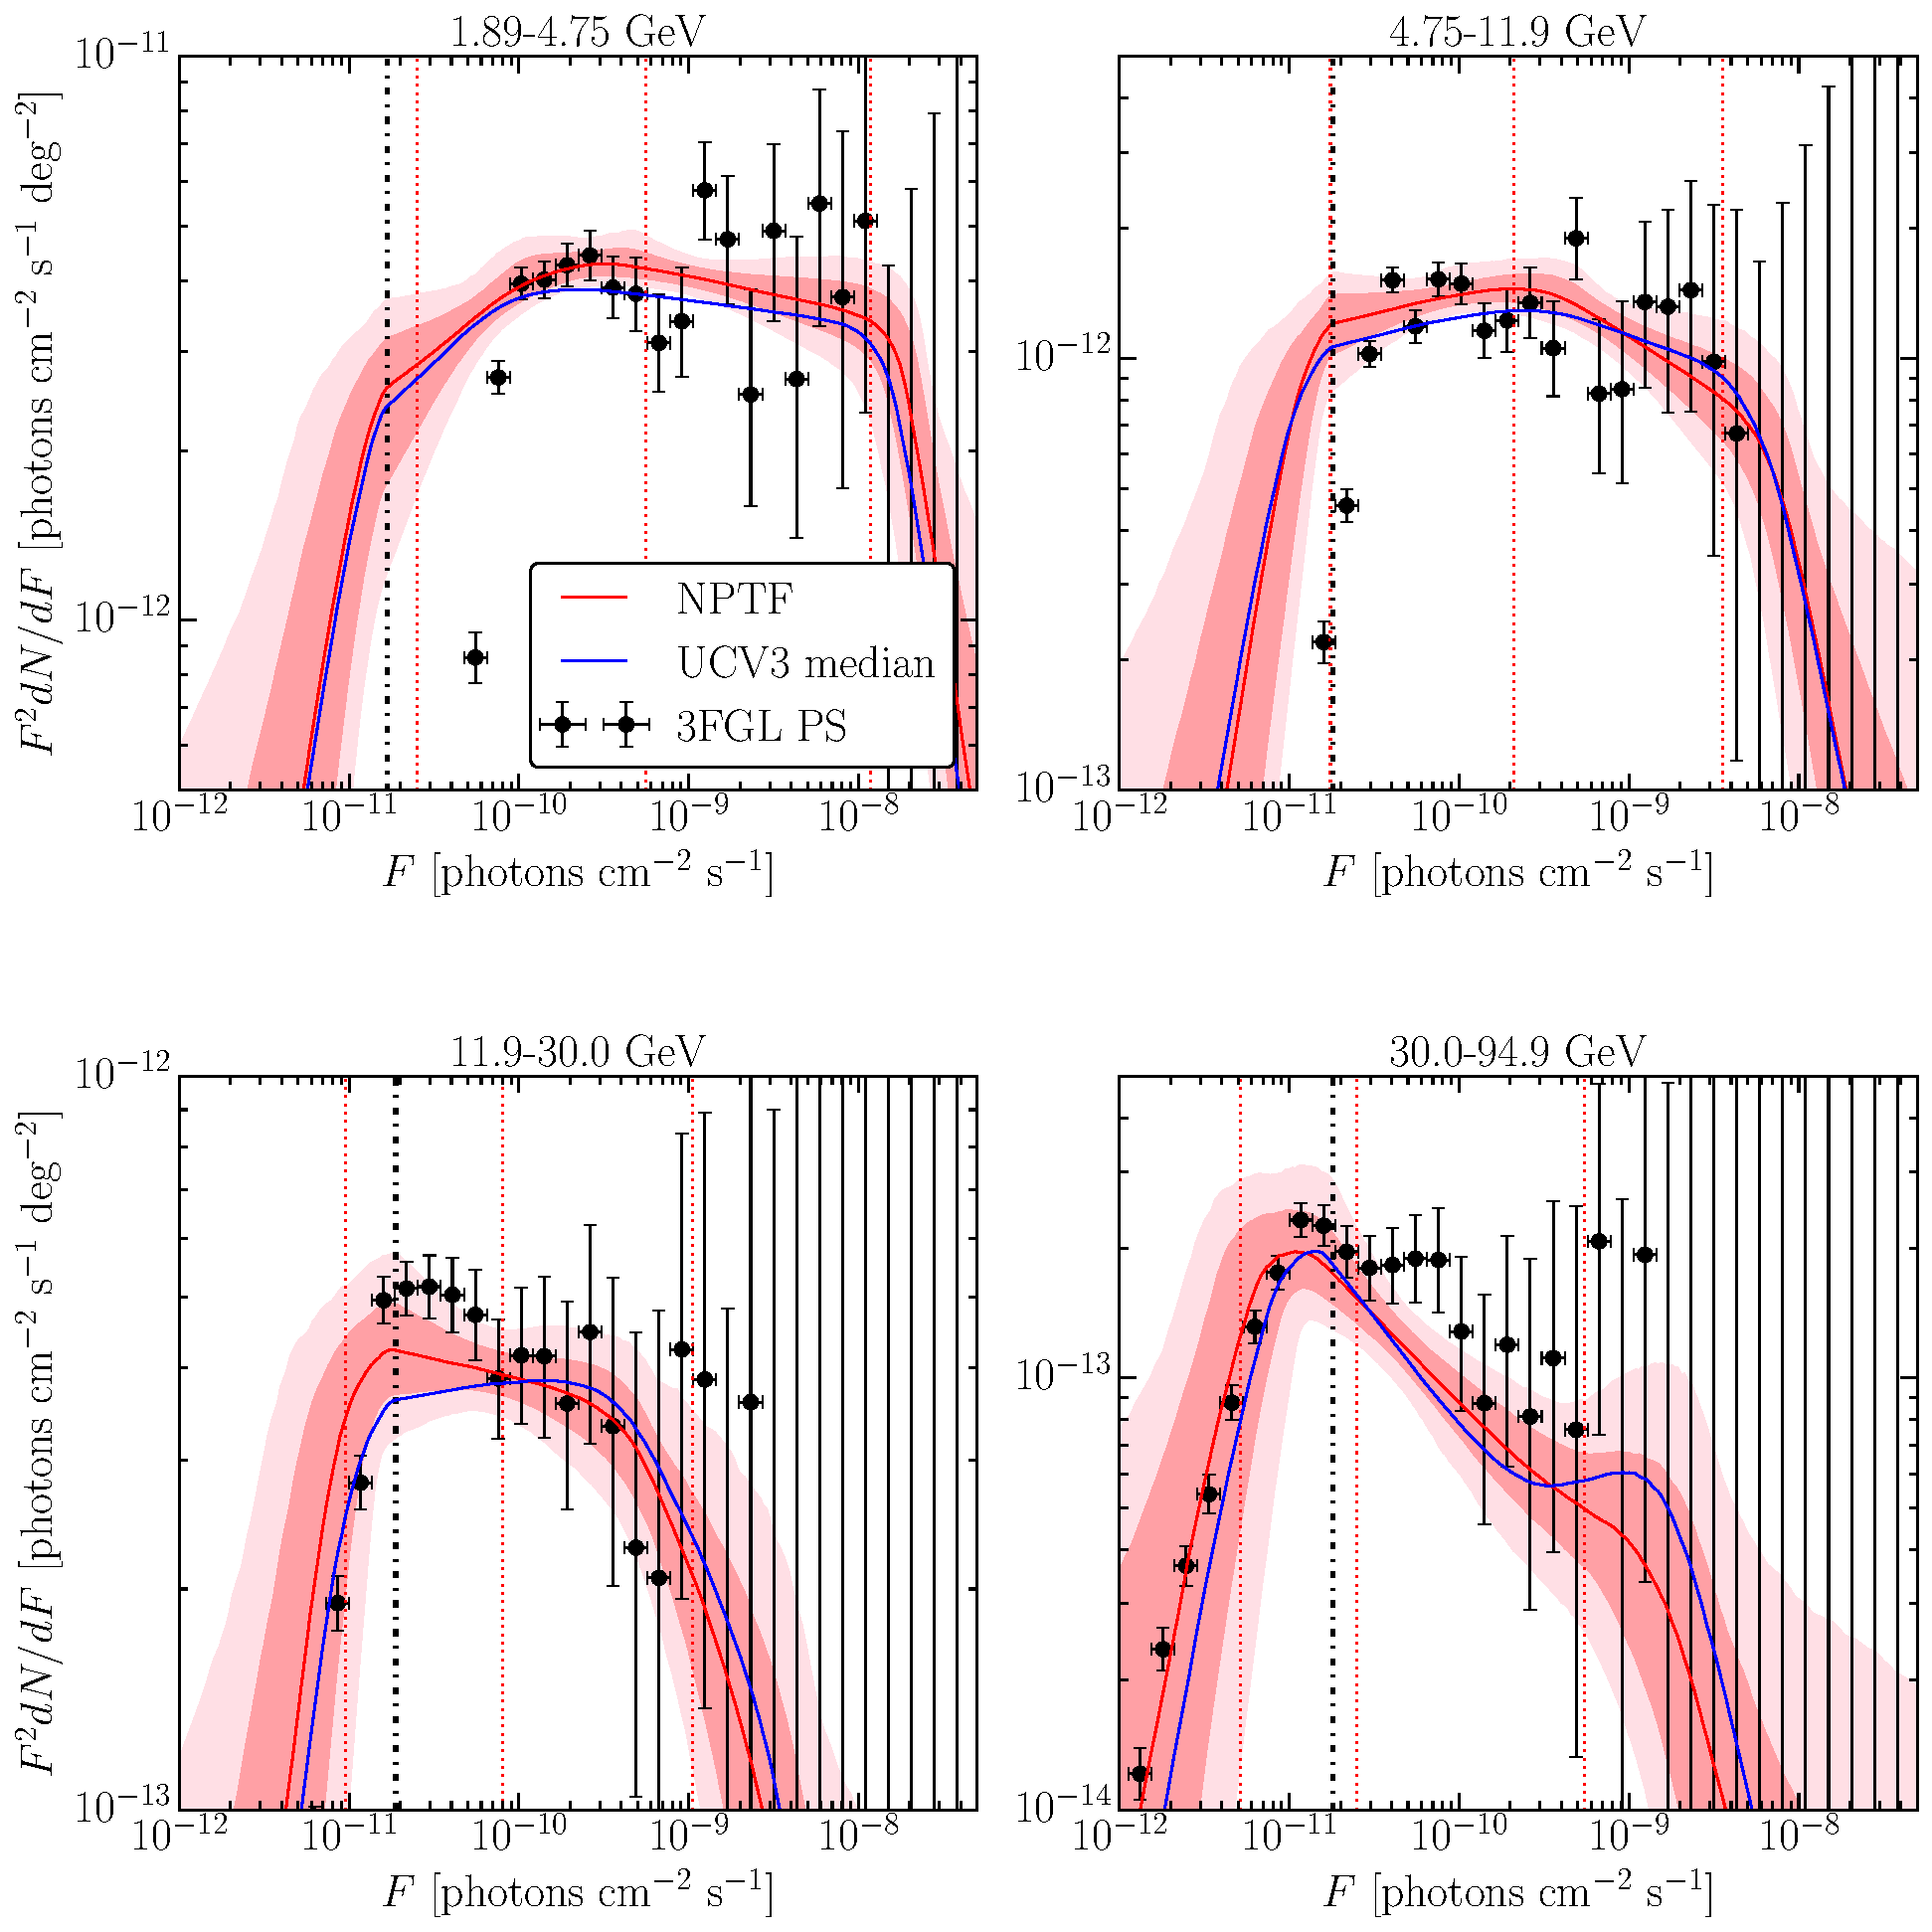
\includegraphics[width=\textwidth]{ch-igrb/plots/UCV_p8_m10-dnds.pdf} 
%    \caption{Best-fit source-count distribution using the Pass 8 {\it ultracleanveto} PSF3 data set and \texttt{p8r2} foreground model, but with $|b| > 10^\circ$.  The median source-count distribution for the benchmark analysis is shown in blue. (Formatted as in Fig.~\ref{fig:dndsdata}.)}
%    \label{fig:dndsdata_m10}
% \end{figure*}
% \clearpage}

% \afterpage{
% \begin{figure*}[phtb] %  figure placement: here, top, bottom, or page
%    \centering
%    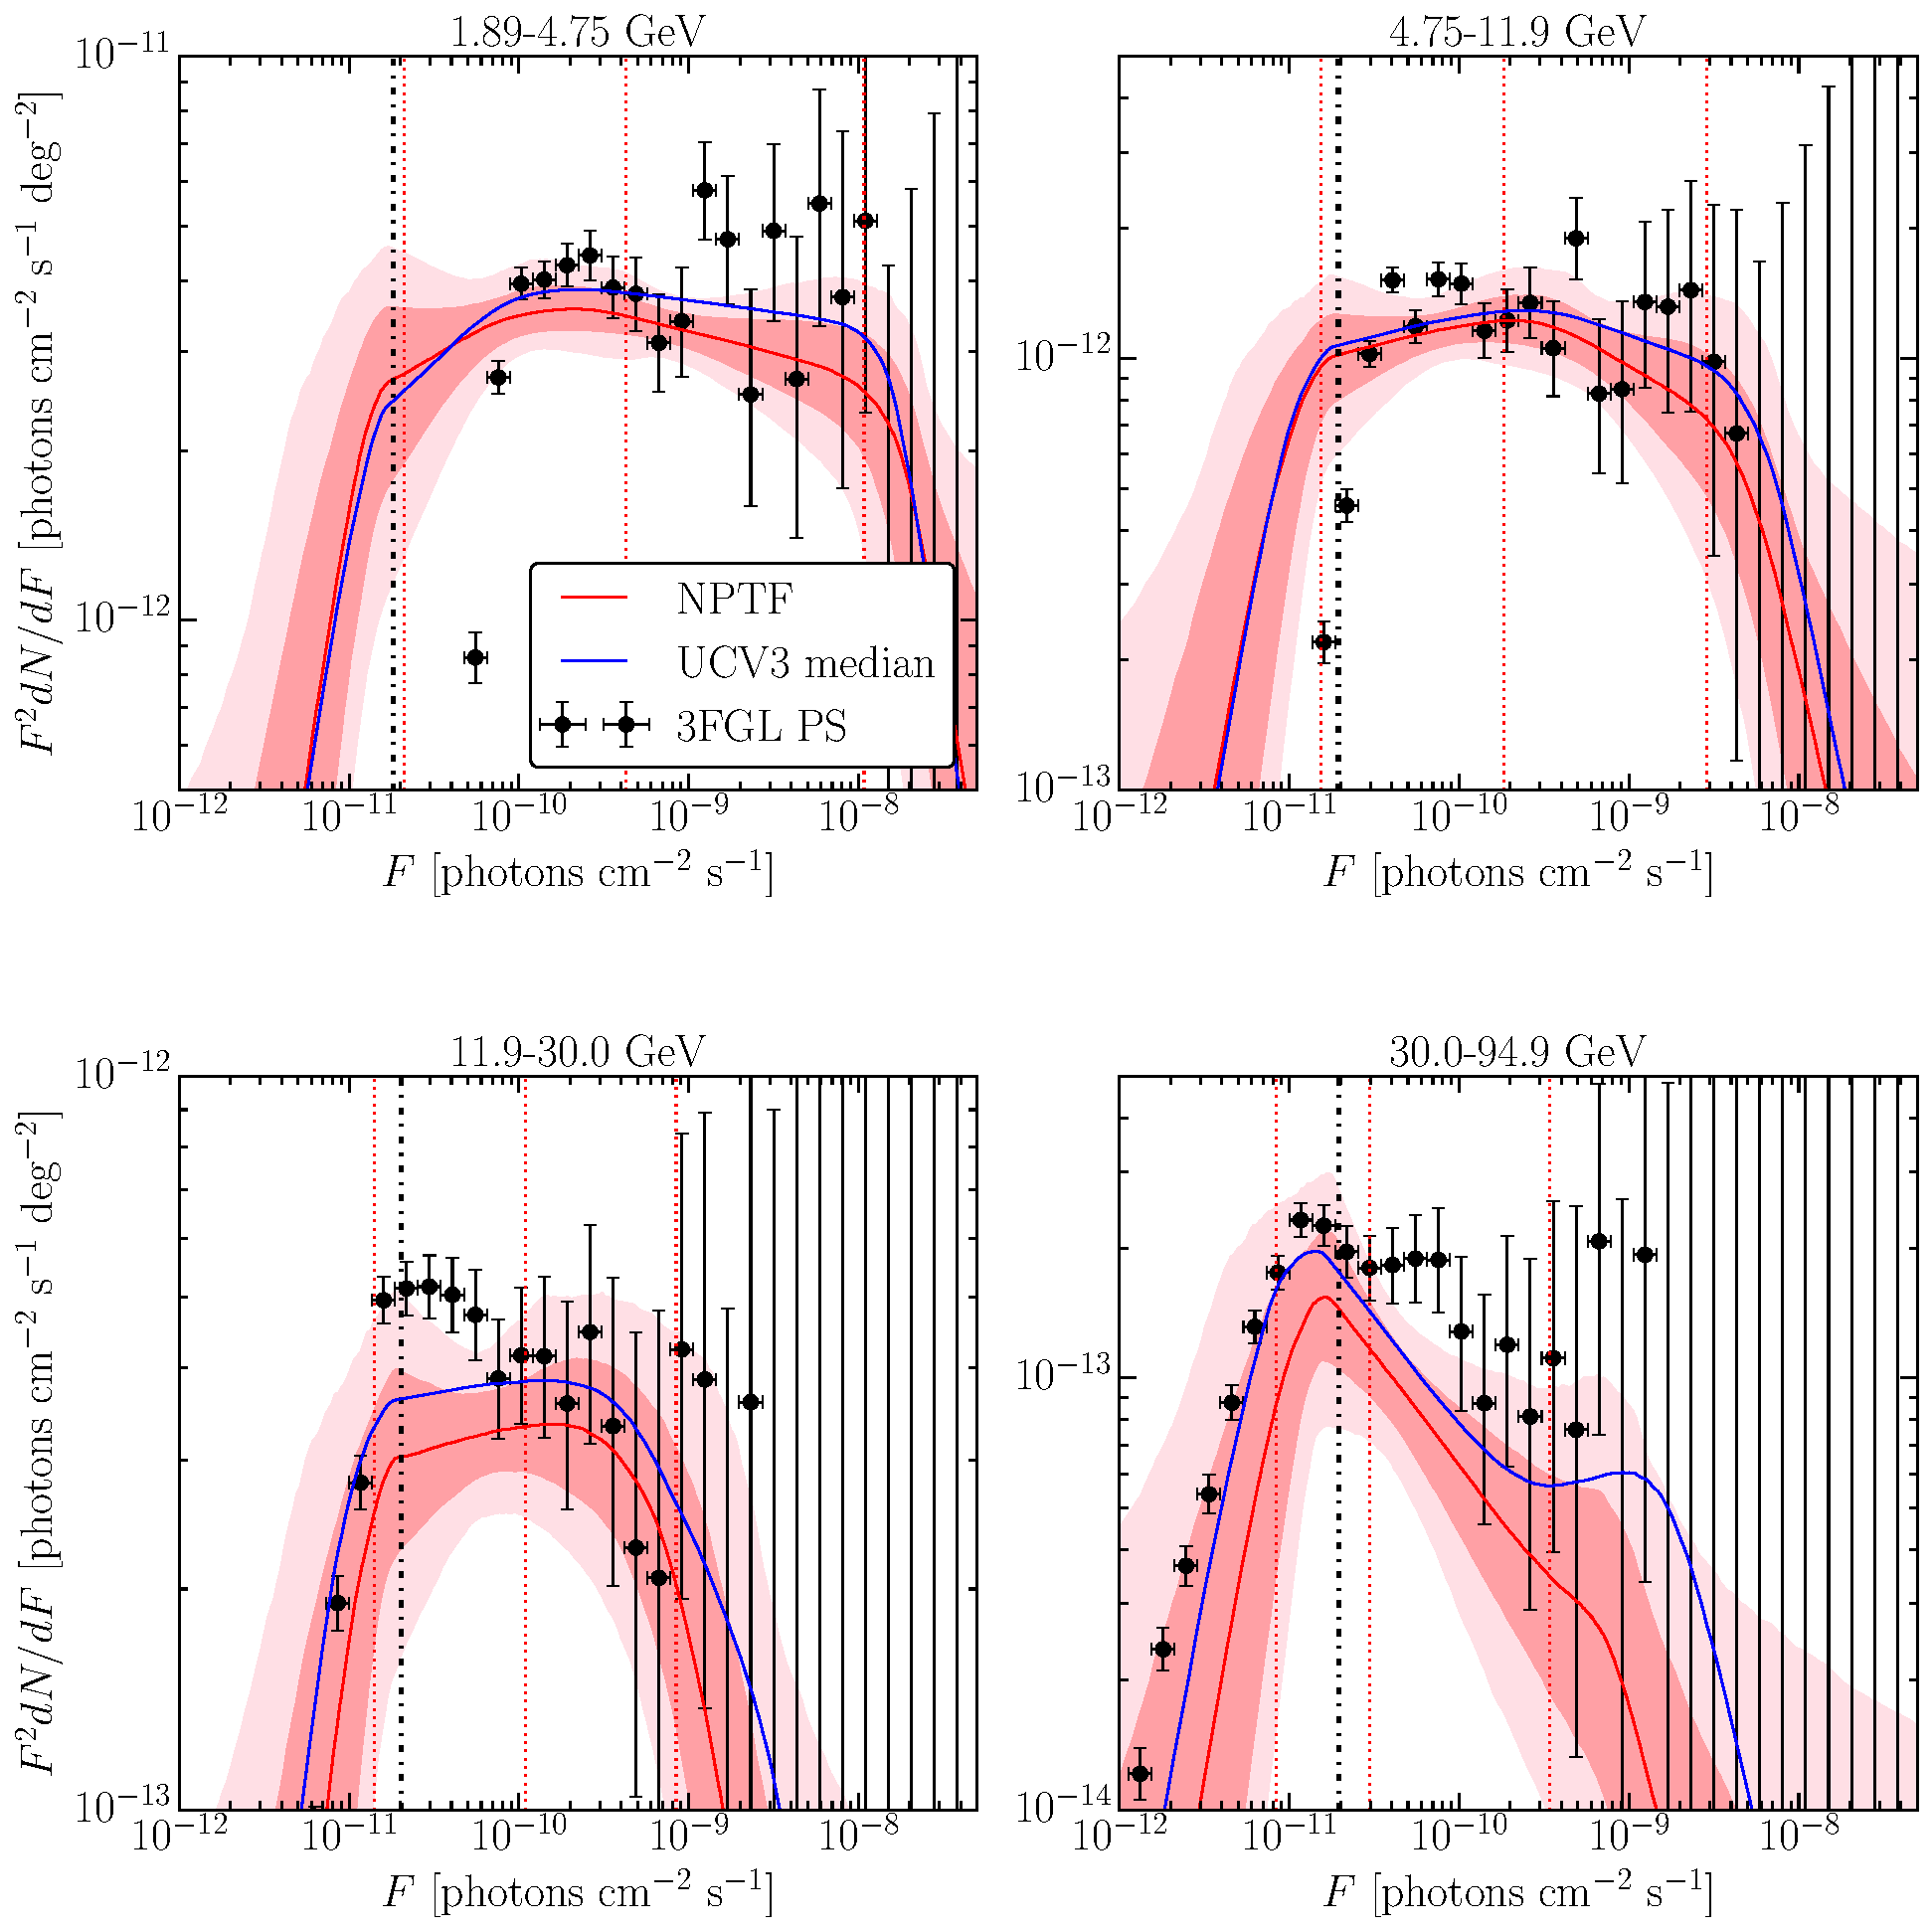
\includegraphics[width=\textwidth]{ch-igrb/plots/UCV_p8_north-dnds.pdf} 
%    \caption{Best-fit source-count distribution using the Pass 8 {\it ultracleanveto} PSF3 data set and \texttt{p8r2} foreground model, but with $b > 30^\circ$.  The median source-count distribution for the benchmark analysis is shown in blue.  (Formatted as in Fig.~\ref{fig:dndsdata}.)}
%    \label{fig:dndsdata_north}
% \end{figure*}
% \clearpage}

% \afterpage{
% \begin{figure*}[phtb] %  figure placement: here, top, bottom, or page
%    \centering
%    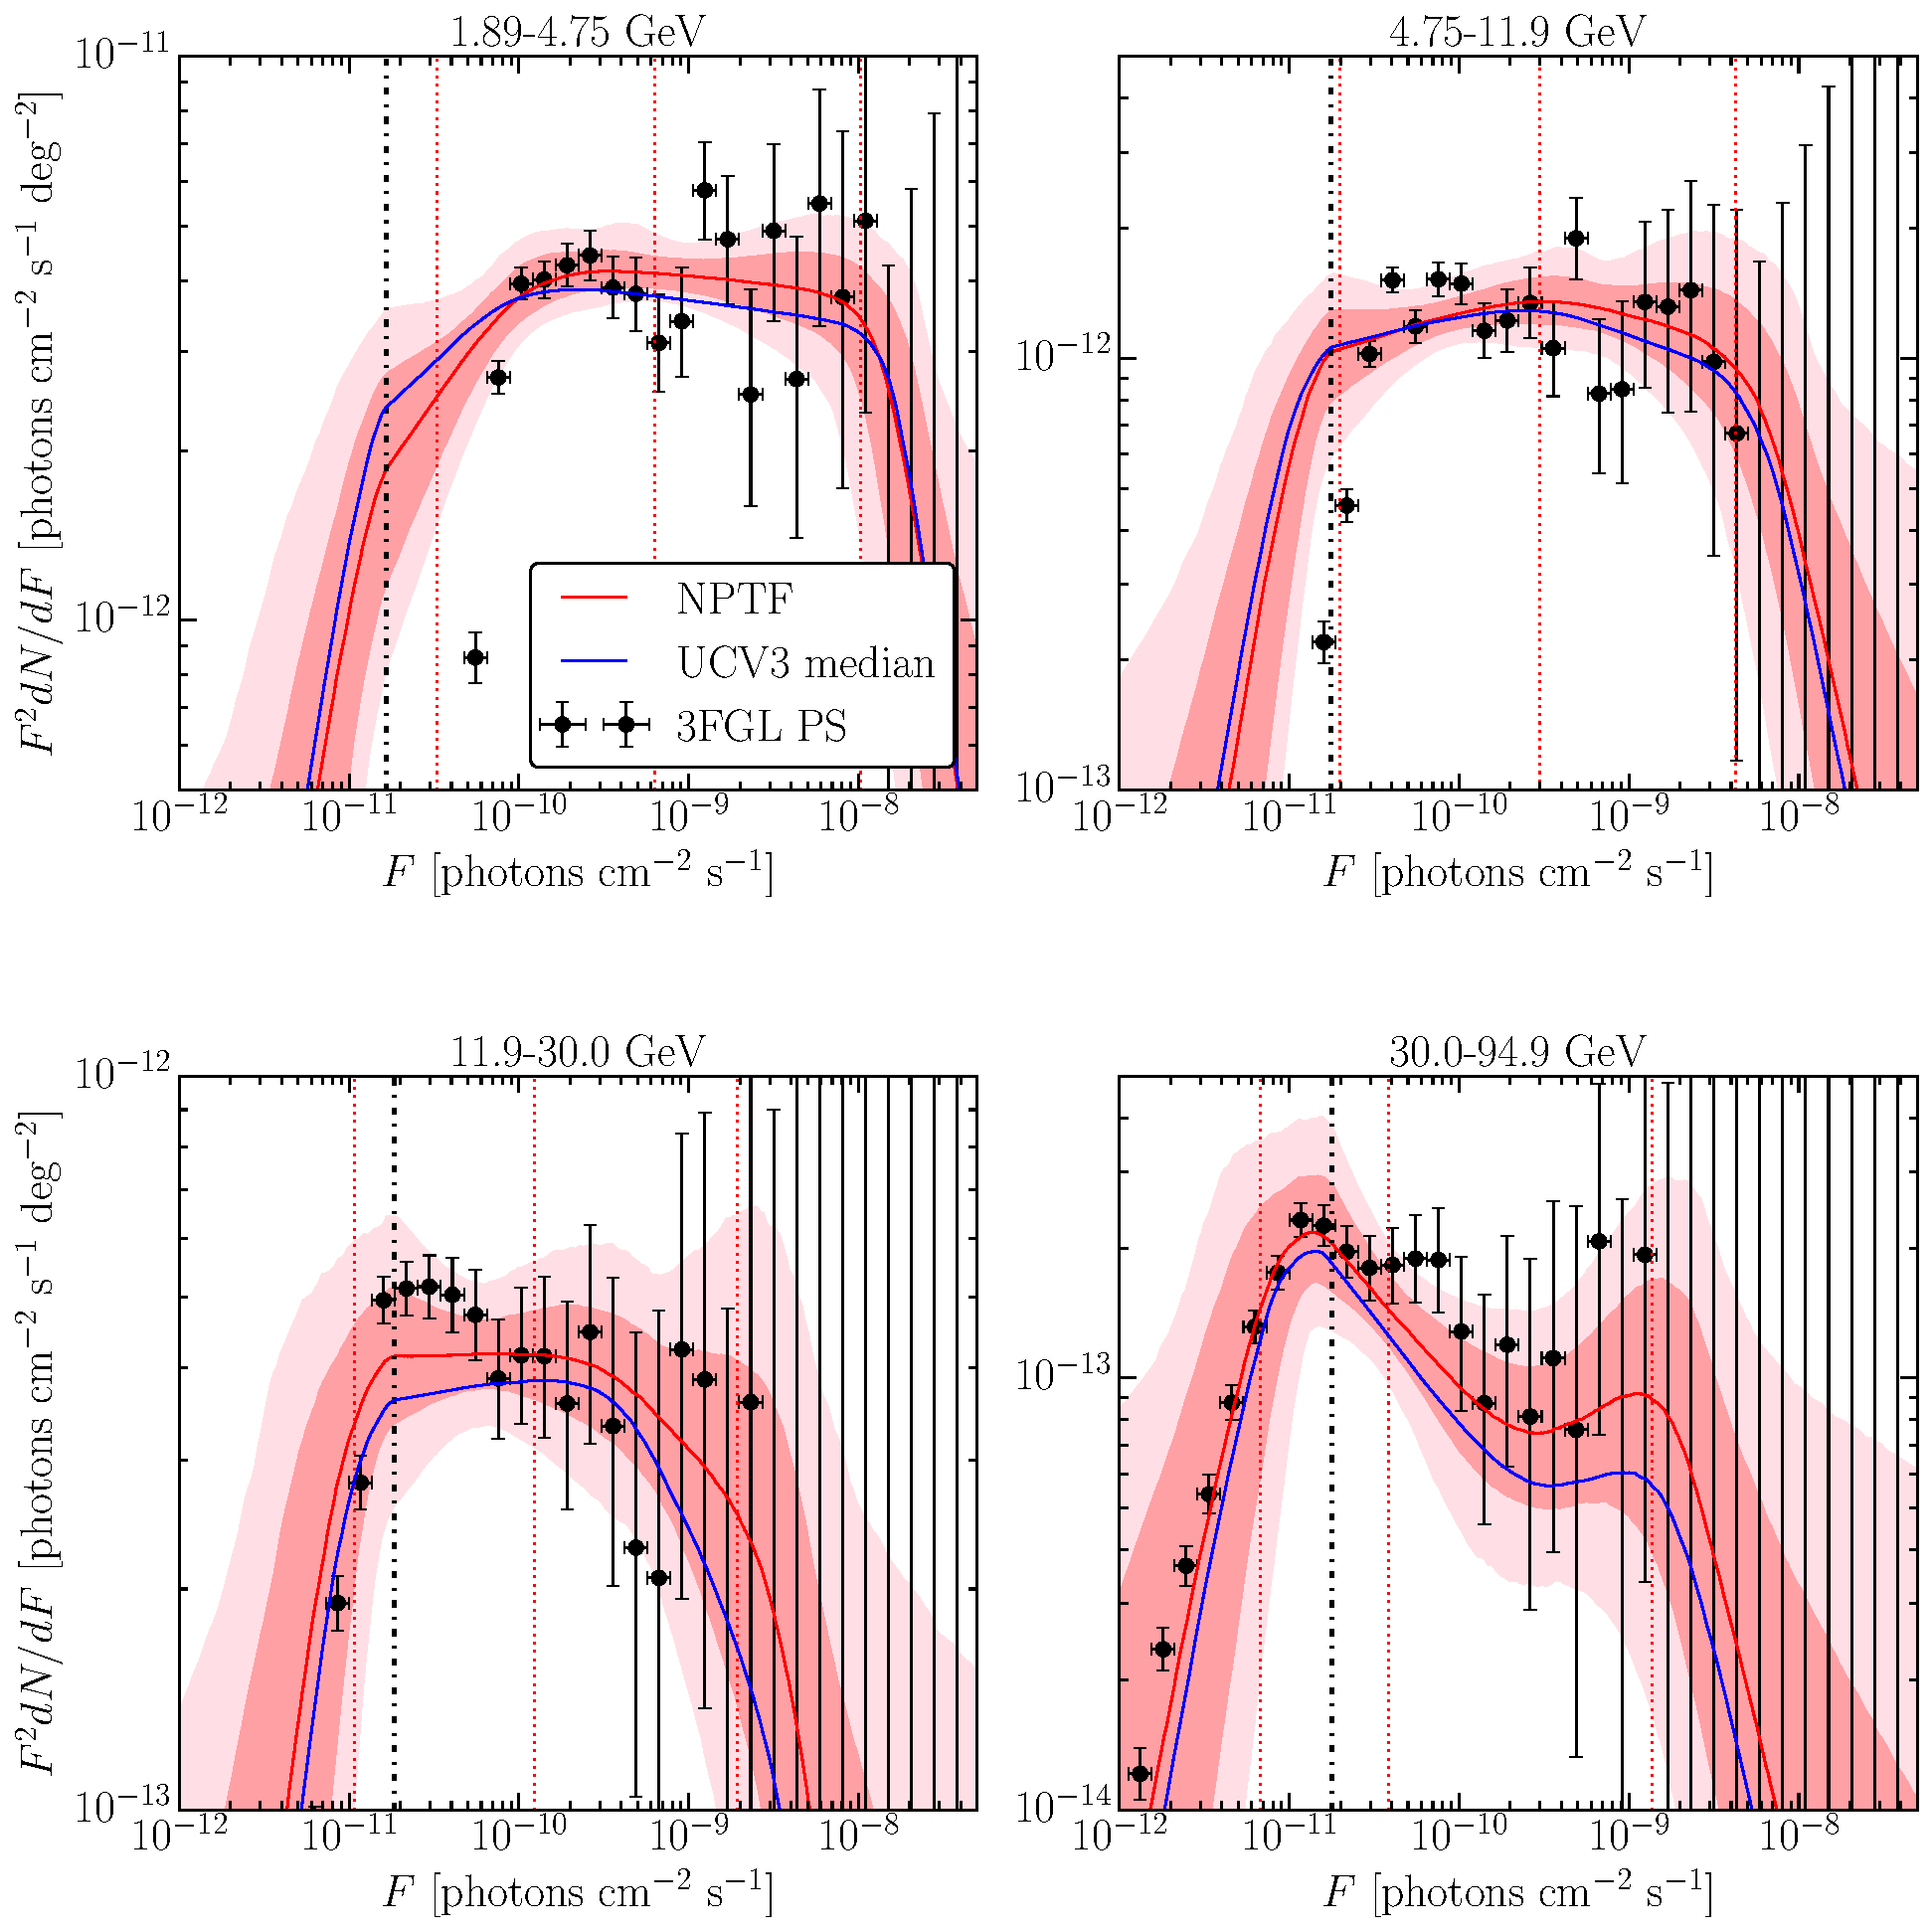
\includegraphics[width=\textwidth]{ch-igrb/plots/UCV_p8_south-dnds.pdf} 
%    \caption{Best-fit source-count distribution using the Pass 8 {\it ultracleanveto} PSF3 data set and \texttt{p8r2} foreground model, but with $b < -30^\circ$.  The median source-count distribution for the benchmark analysis is shown in blue. (Formatted as in Fig.~\ref{fig:dndsdata}.)}
%    \label{fig:dndsdata_south}
% \end{figure*}
% \clearpage}


% \afterpage{
% \begin{figure*}[phtb] %  figure placement: here, top, bottom, or page
%    \centering
%    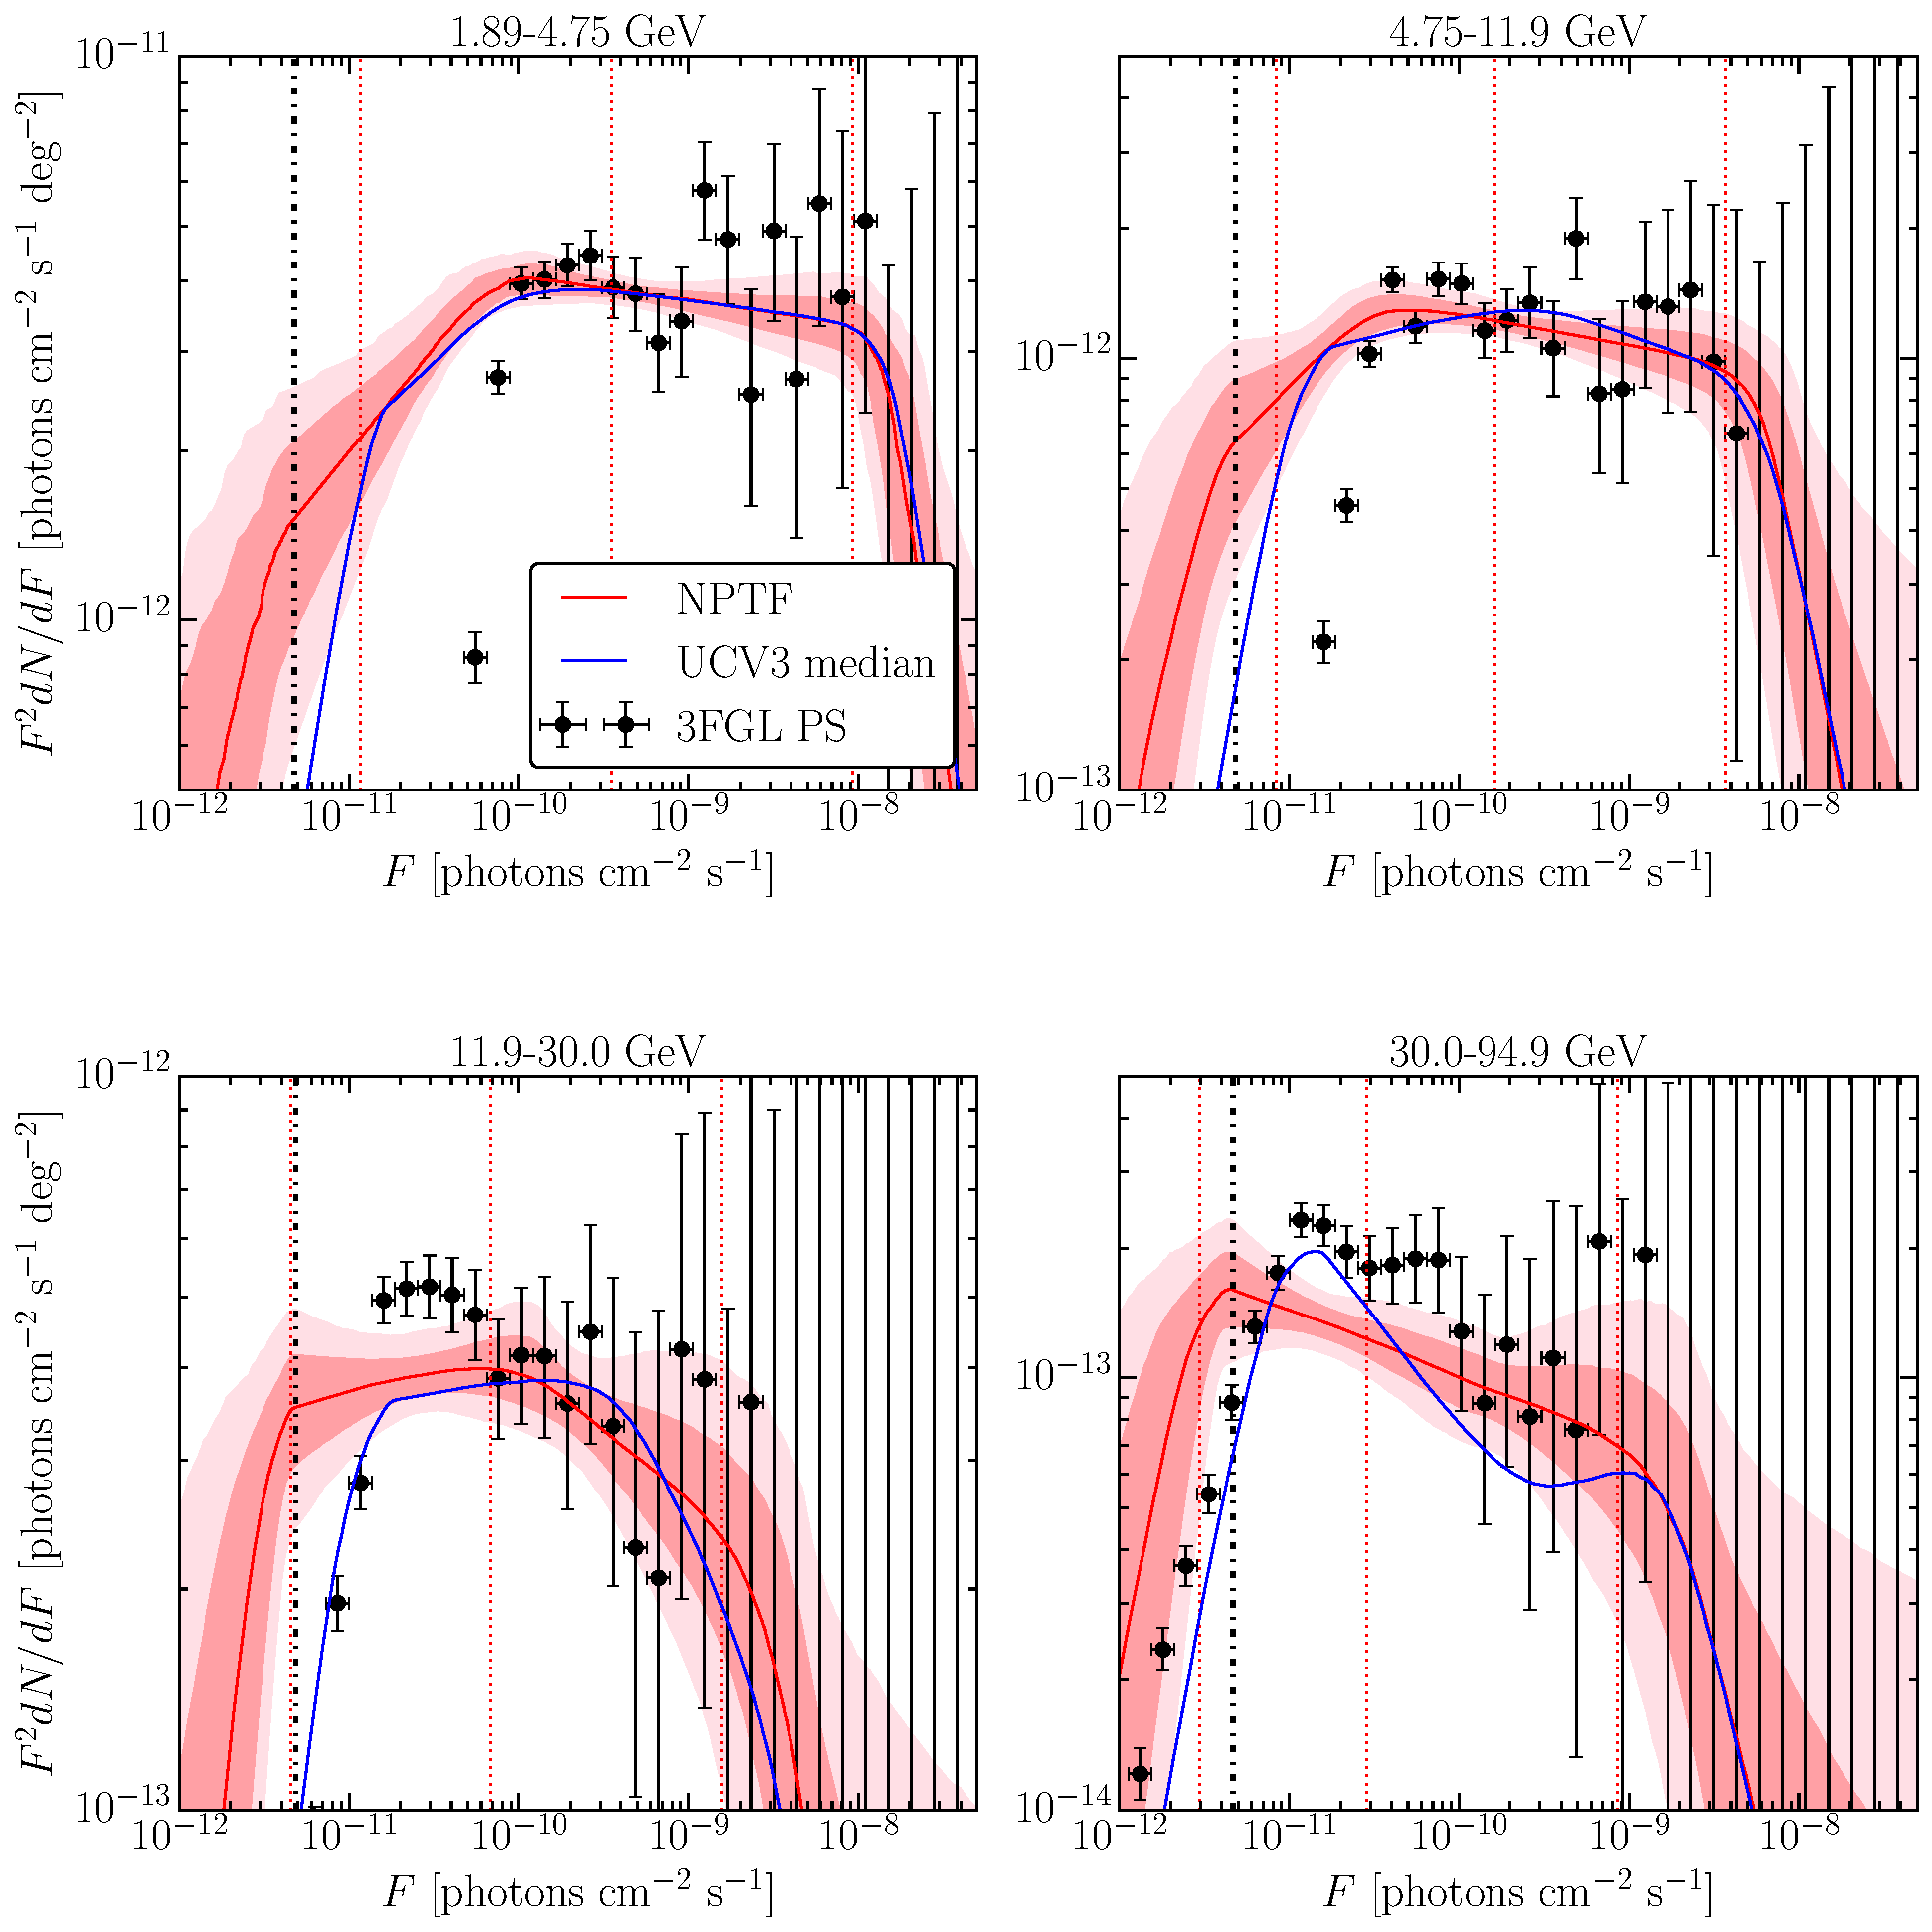
\includegraphics[width=\textwidth]{ch-igrb/plots/Q3_p8-dnds.pdf} 
%    \caption{Best-fit source-count distribution using the top three quartiles of Pass 8 {\it source} data and the \texttt{p8r2} foreground model.  The median source-count distribution for the benchmark analysis is shown in  blue.  (Formatted as in Fig.~\ref{fig:dndsdata}.)}
%    \label{fig:dndsdata_source}
% \end{figure*}
% \clearpage}

% \afterpage{
% \begin{figure*}[phtb] %  figure placement: here, top, bottom, or page
%    \centering
%    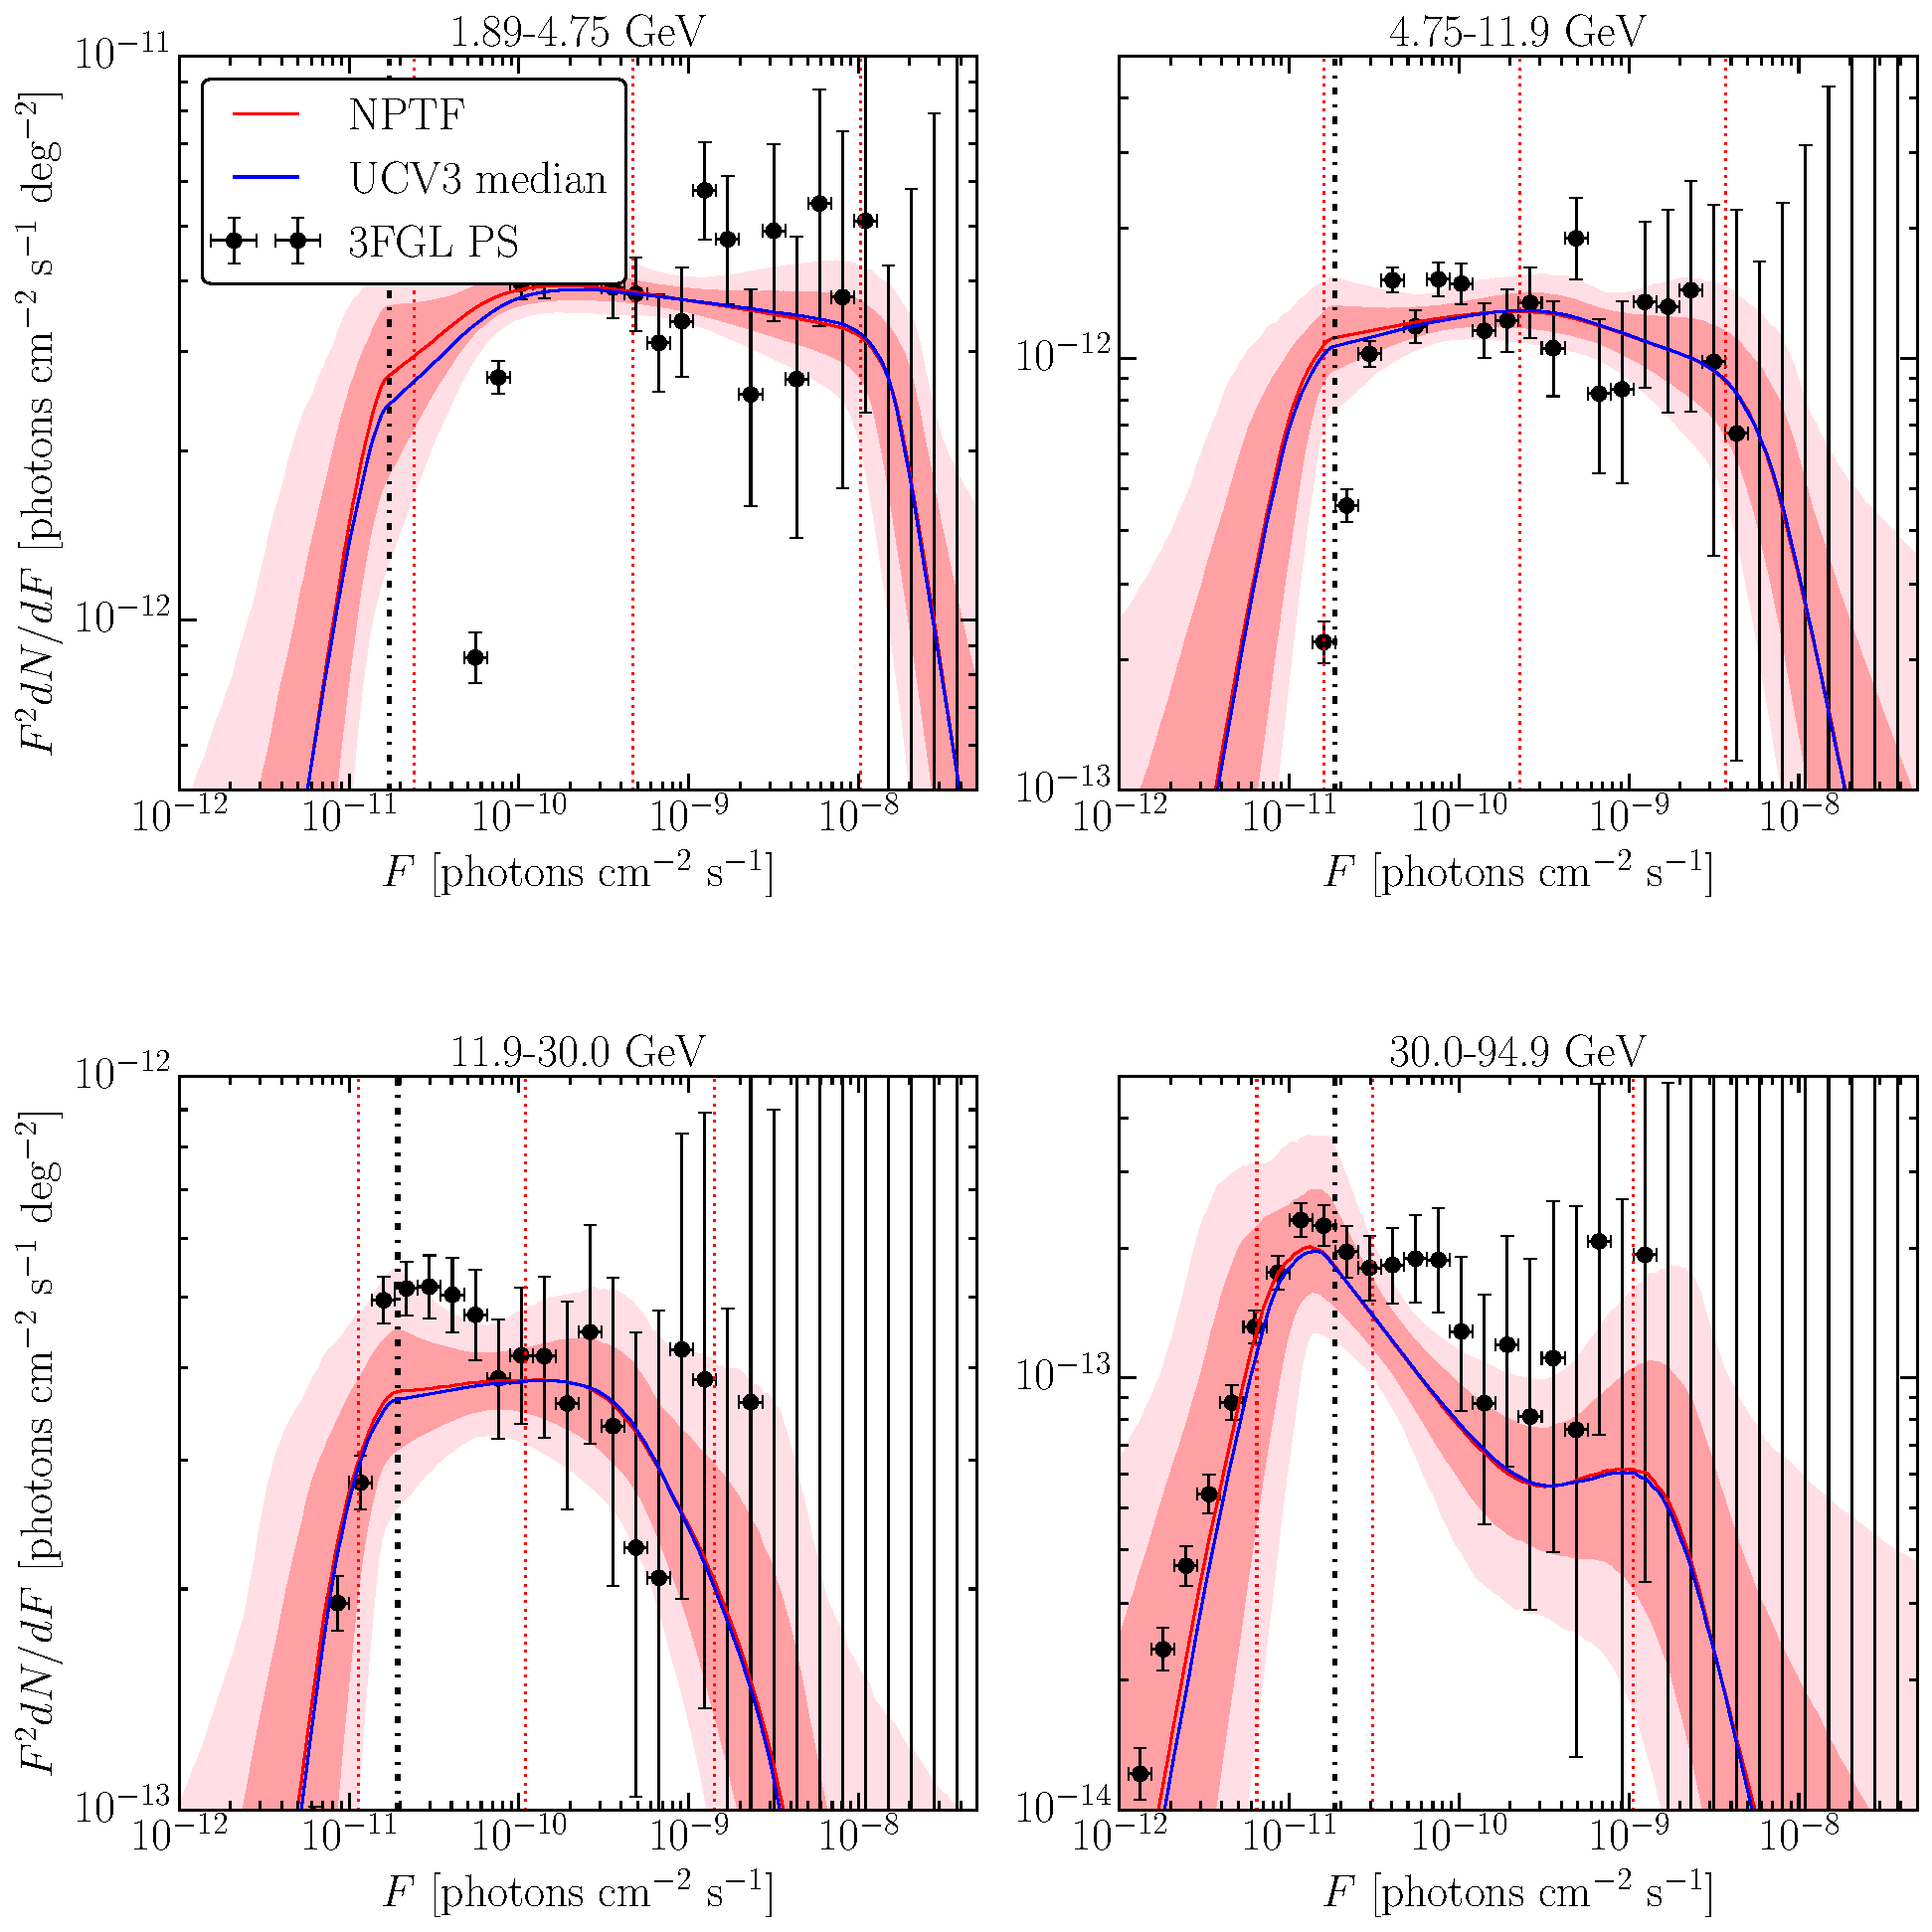
\includegraphics[width=\textwidth]{ch-igrb/plots/UCV_p6-dnds.pdf} 
%    \caption{Best-fit source-count distribution using the Pass 8 {\it ultracleanveto} PSF3 data set and \texttt{p6v11} foreground model.  The median source-count distribution for the benchmark analysis is shown in blue. (Formatted as in Fig.~\ref{fig:dndsdata}.)}
%    \label{fig:dndsdata_p6}
% \end{figure*}
% \clearpage}

% \afterpage{
% \begin{figure*}[phtb] %  figure placement: here, top, bottom, or page
%    \centering
%    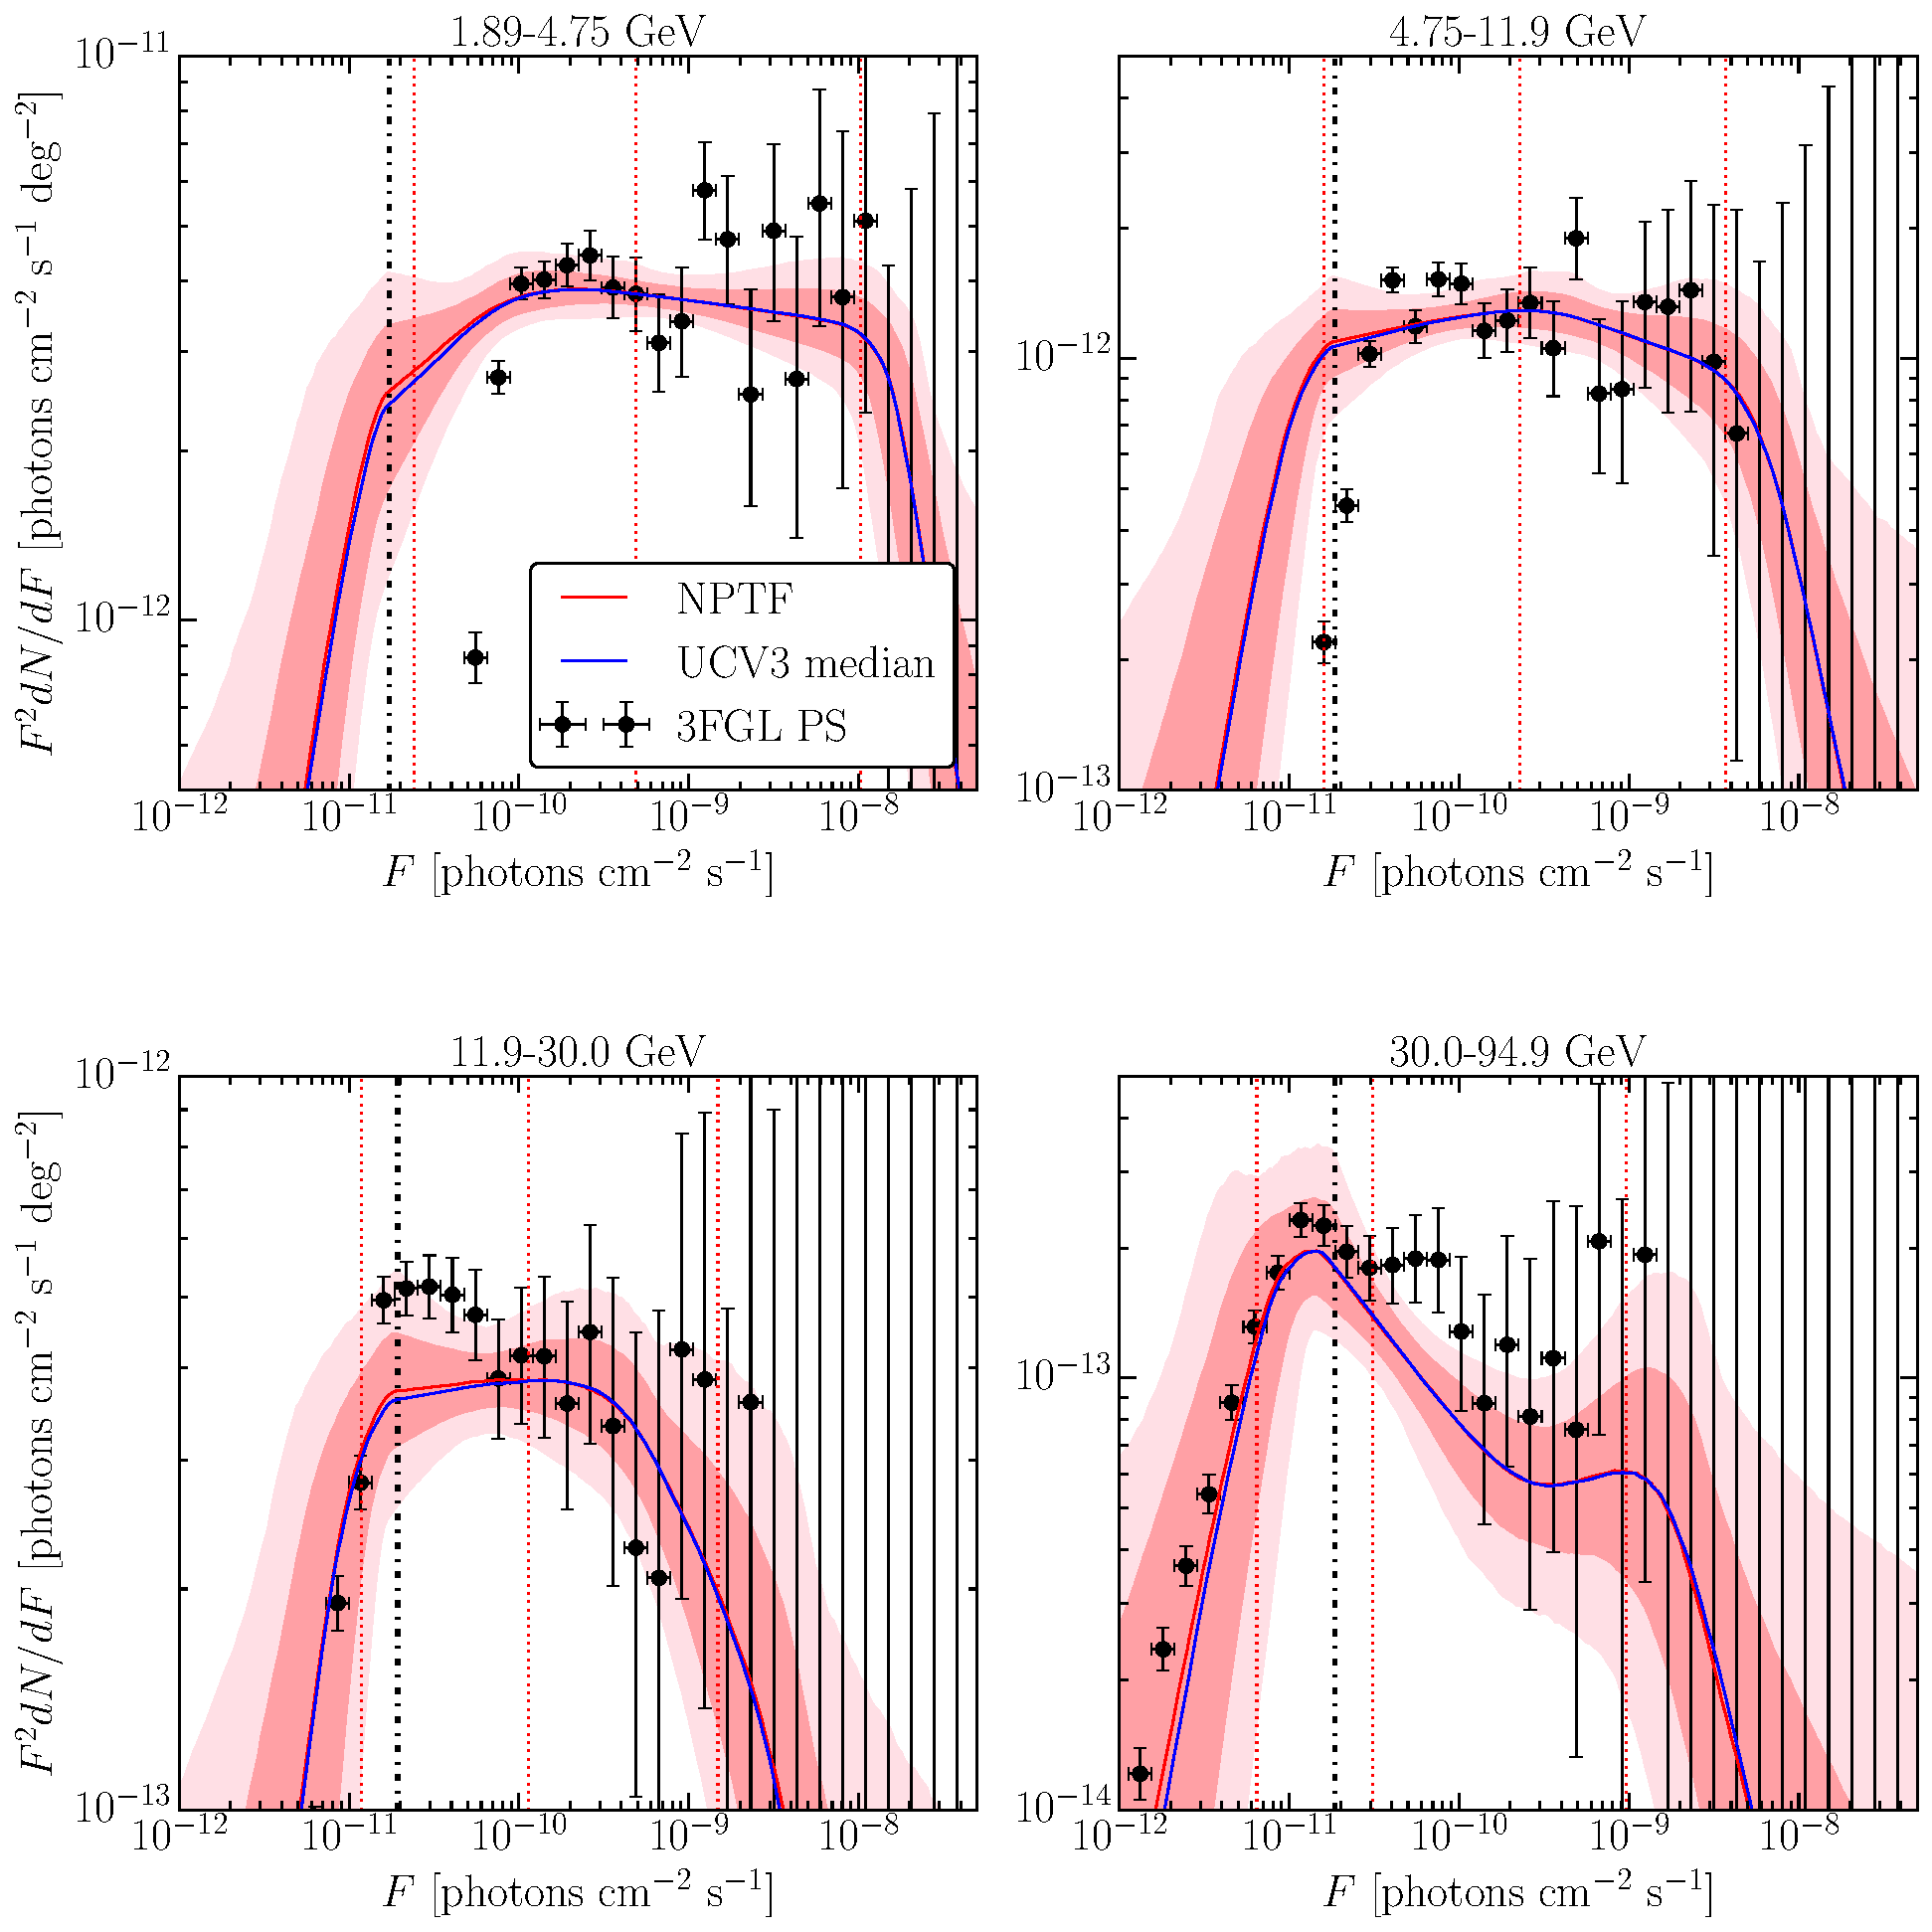
\includegraphics[width=\textwidth]{ch-igrb/plots/UCV_p7-dnds.pdf} 
%    \caption{Best-fit source-count distribution using the Pass 8 {\it ultracleanveto} PSF3 data set and \texttt{p7v6} foreground model.  The median source-count distribution for the benchmark analysis is shown in blue. (Formatted as in Fig.~\ref{fig:dndsdata}.)}
%    \label{fig:dndsdata_p7}
% \end{figure*}
% \clearpage}

% \afterpage{
% \begin{figure*}[phtb] %  figure placement: here, top, bottom, or page
%    \centering
%    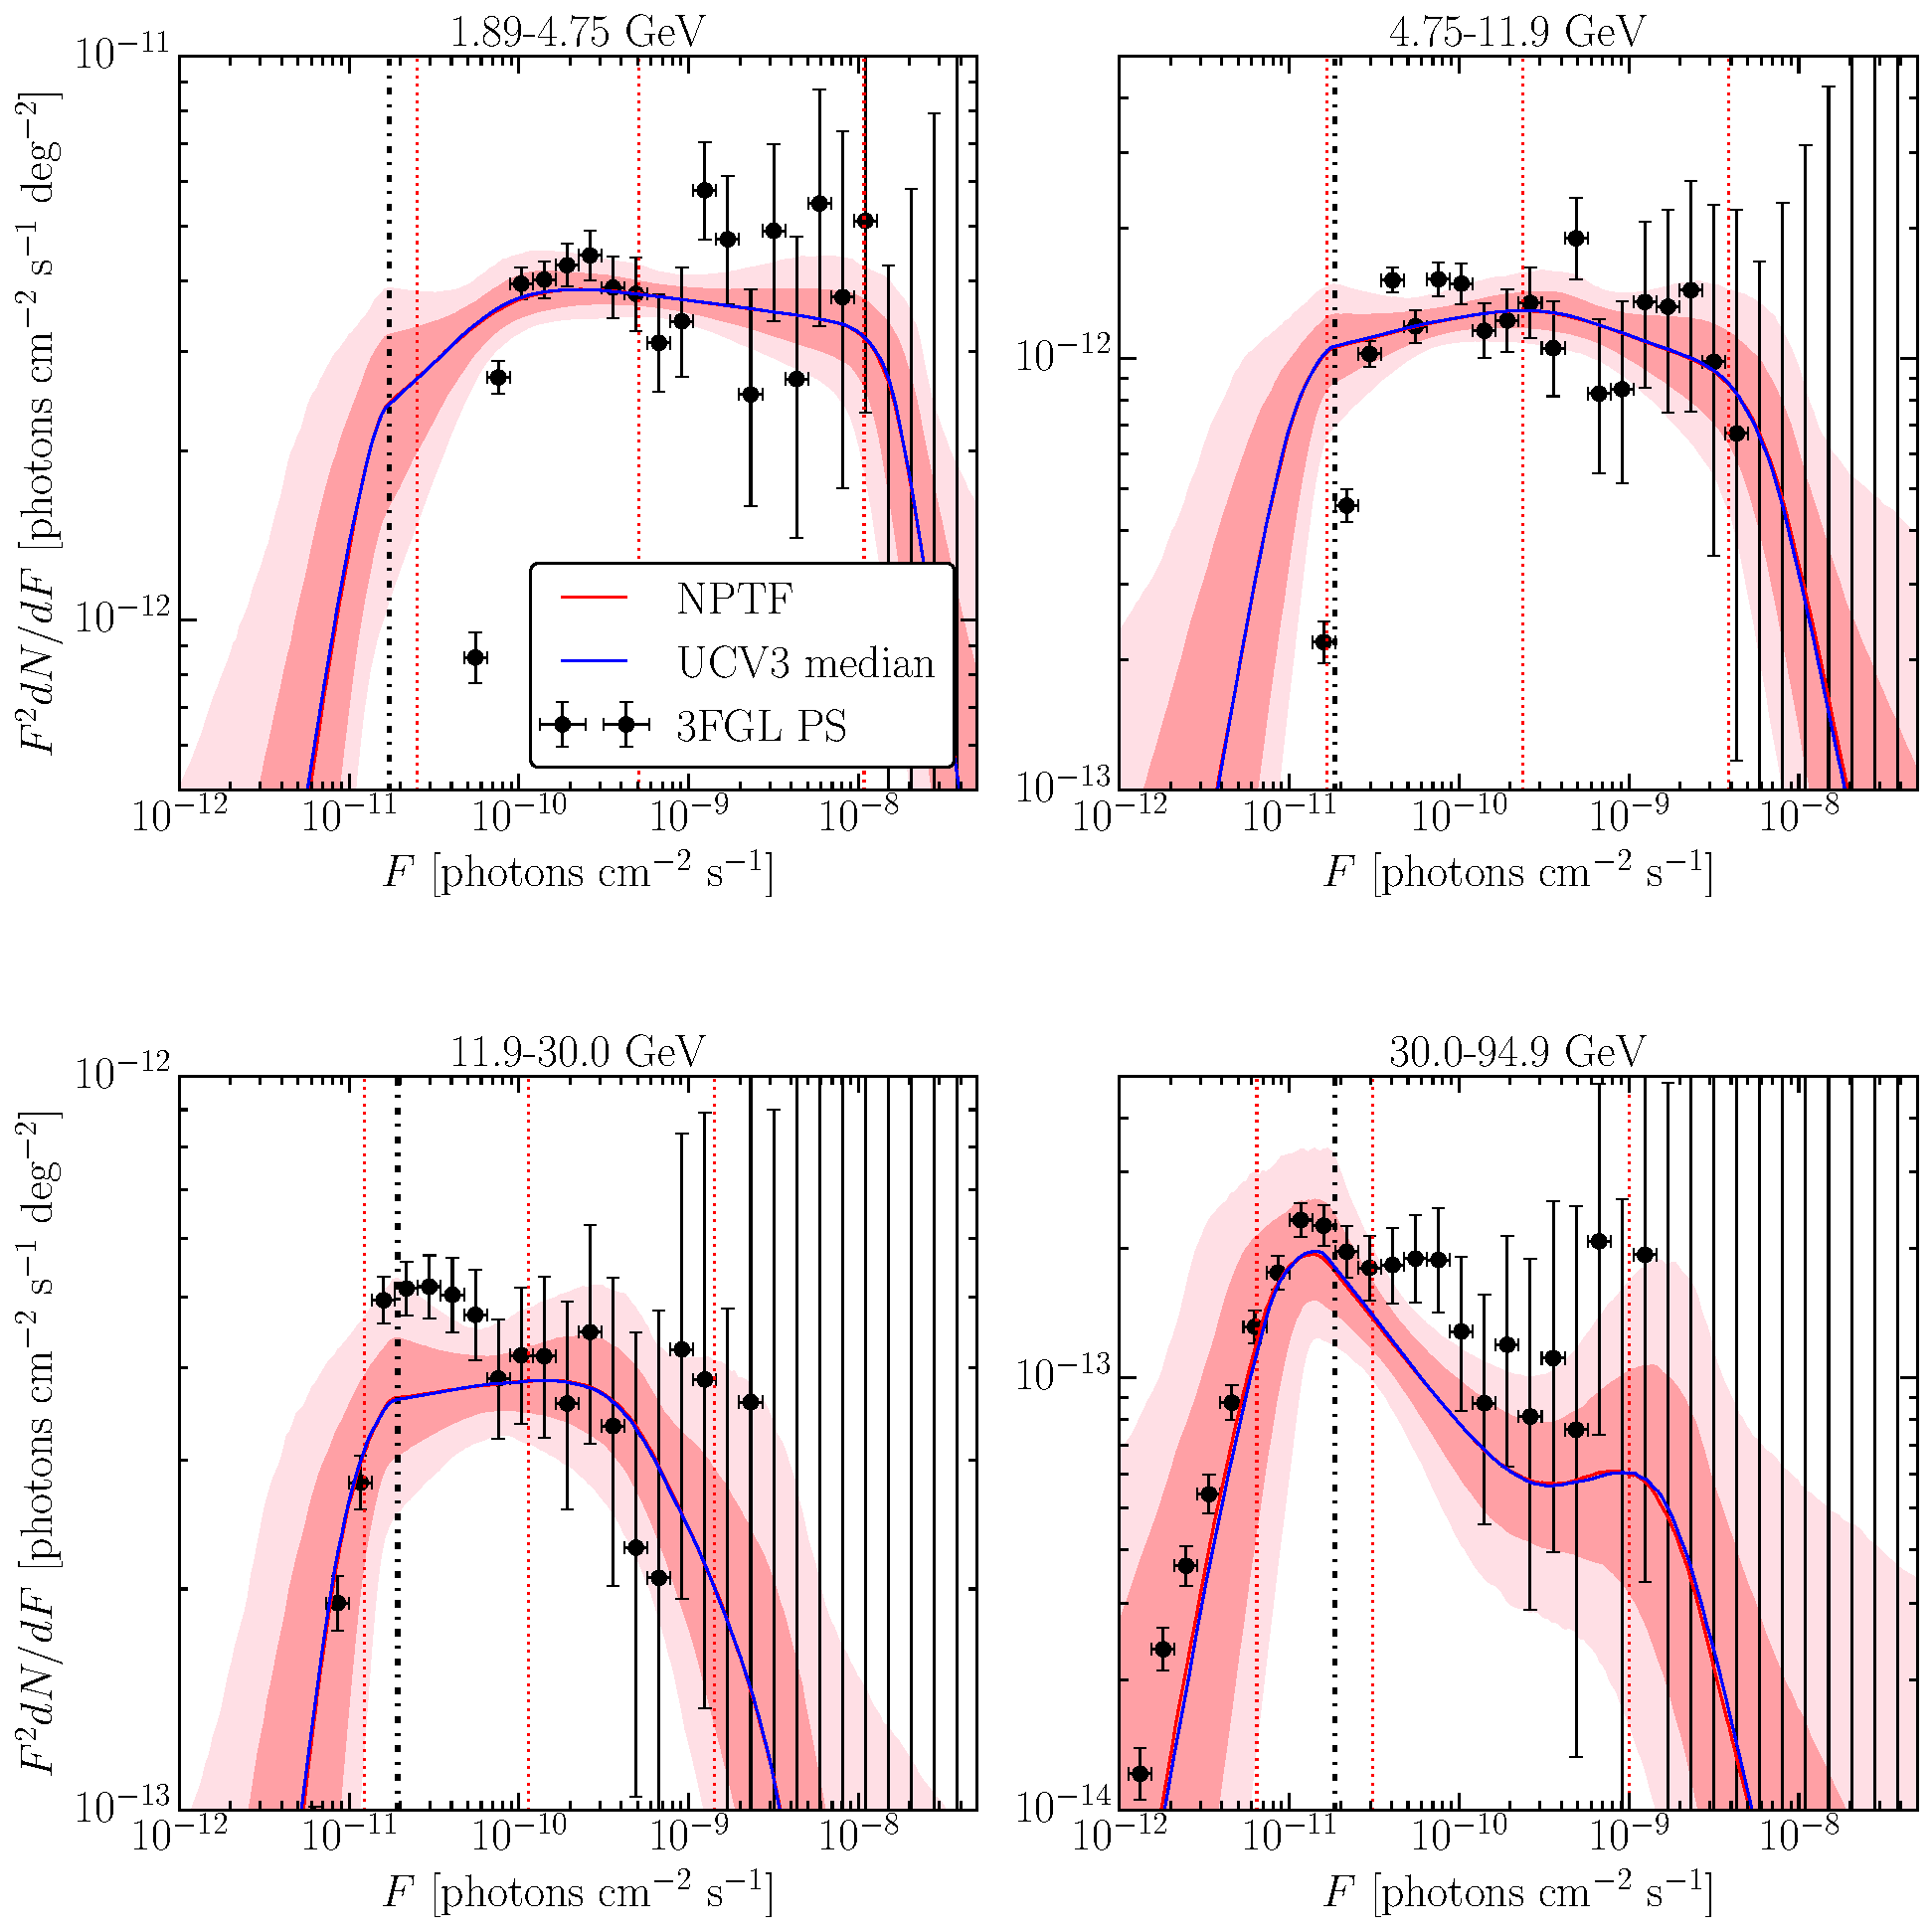
\includegraphics[width=\textwidth]{ch-igrb/plots/ucv_p8_nobubs-dnds.pdf} 
%    \caption{Best-fit source-count distribution using the Pass 8 {\it ultracleanveto} PSF3 data set and \texttt{p8r2} foreground model, but removing the \emph{Fermi} bubbles template from the analysis..  The median source-count distribution for the benchmark analysis is shown in blue. (Formatted as in Fig.~\ref{fig:dndsdata}.)}
%    \label{fig:dndsdata_nobub}
% \end{figure*}
% \clearpage}

% \afterpage{
% \begin{figure*}[phtb] %  figure placement: here, top, bottom, or page
%    \centering
%    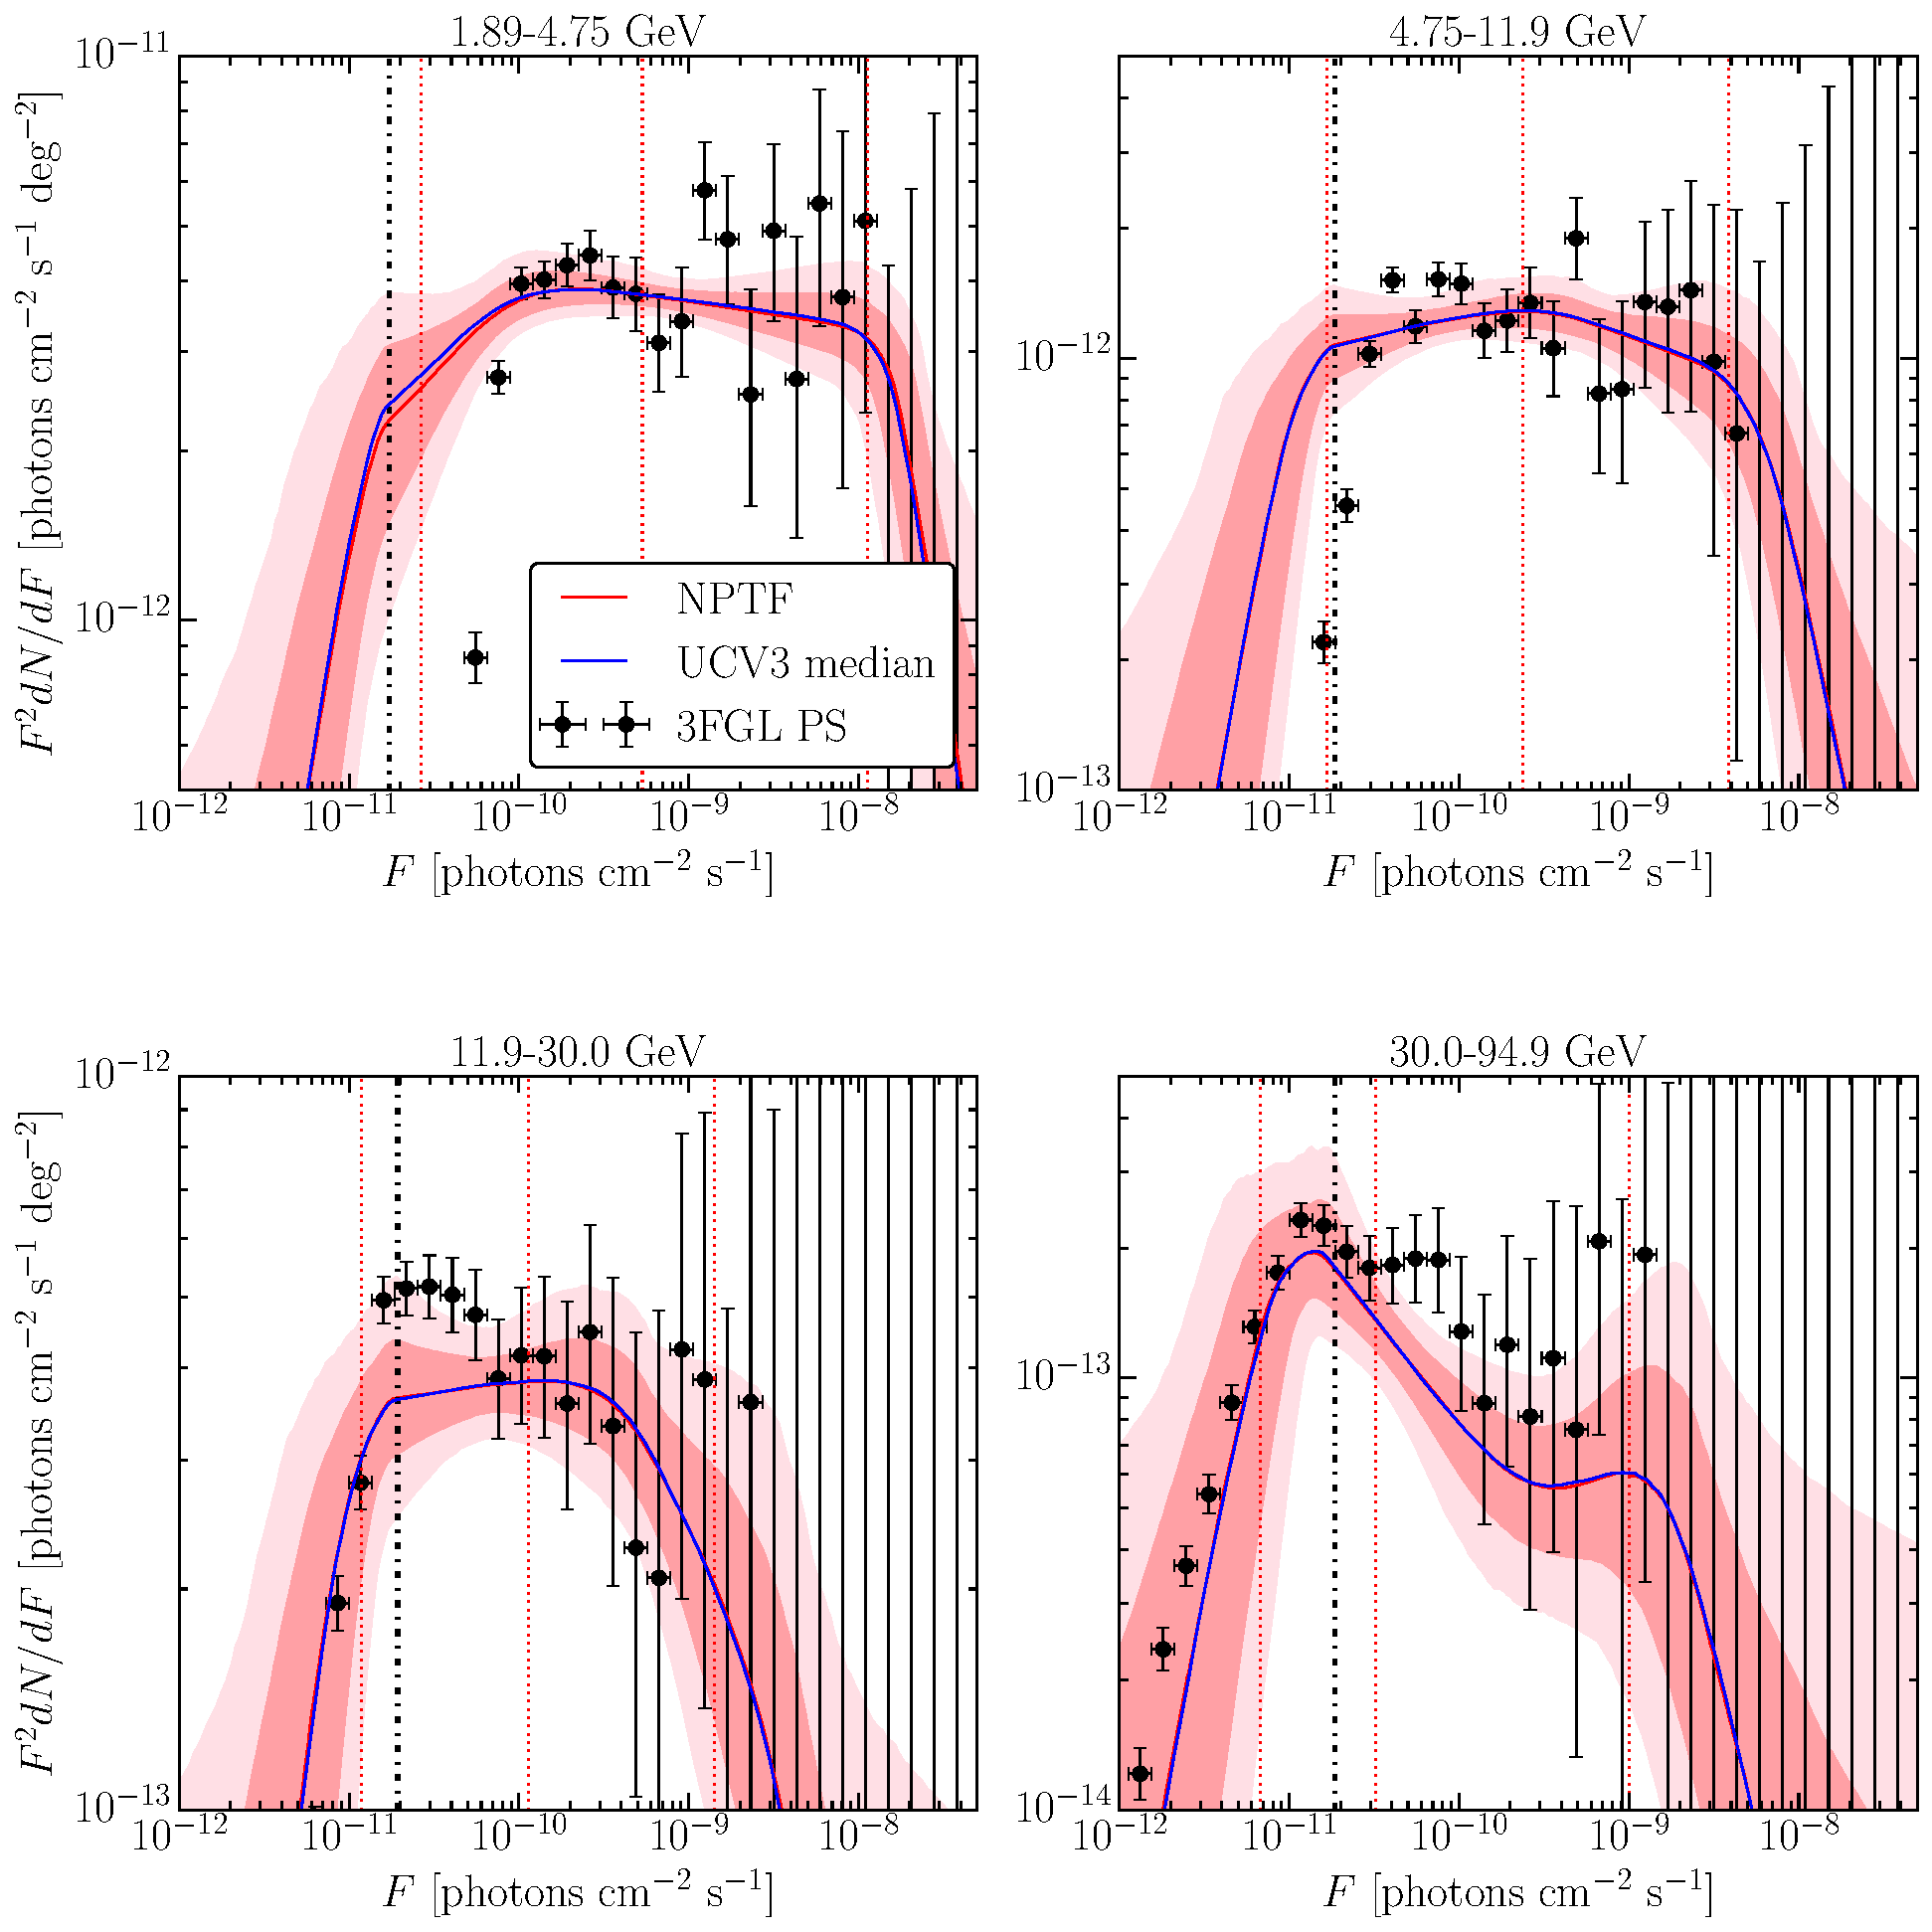
\includegraphics[width=\textwidth]{ch-igrb/plots/UCV_p8_gauss-dnds.pdf} 
%    \caption{Best-fit source-count distribution using the Pass 8 {\it ultracleanveto} PSF3 data set and \texttt{p8r2} foreground model, but with a Gaussian PSF.  The median source-count distribution for the benchmark analysis is shown in blue. (Formatted as in Fig.~\ref{fig:dndsdata}.)}
%    \label{fig:dndsdata_gauss}
% \end{figure*}
% \clearpage}
% \clearpage

% \afterpage{
% \begin{figure*}[phtb] %  figure placement: here, top, bottom, or page
%    \centering
%    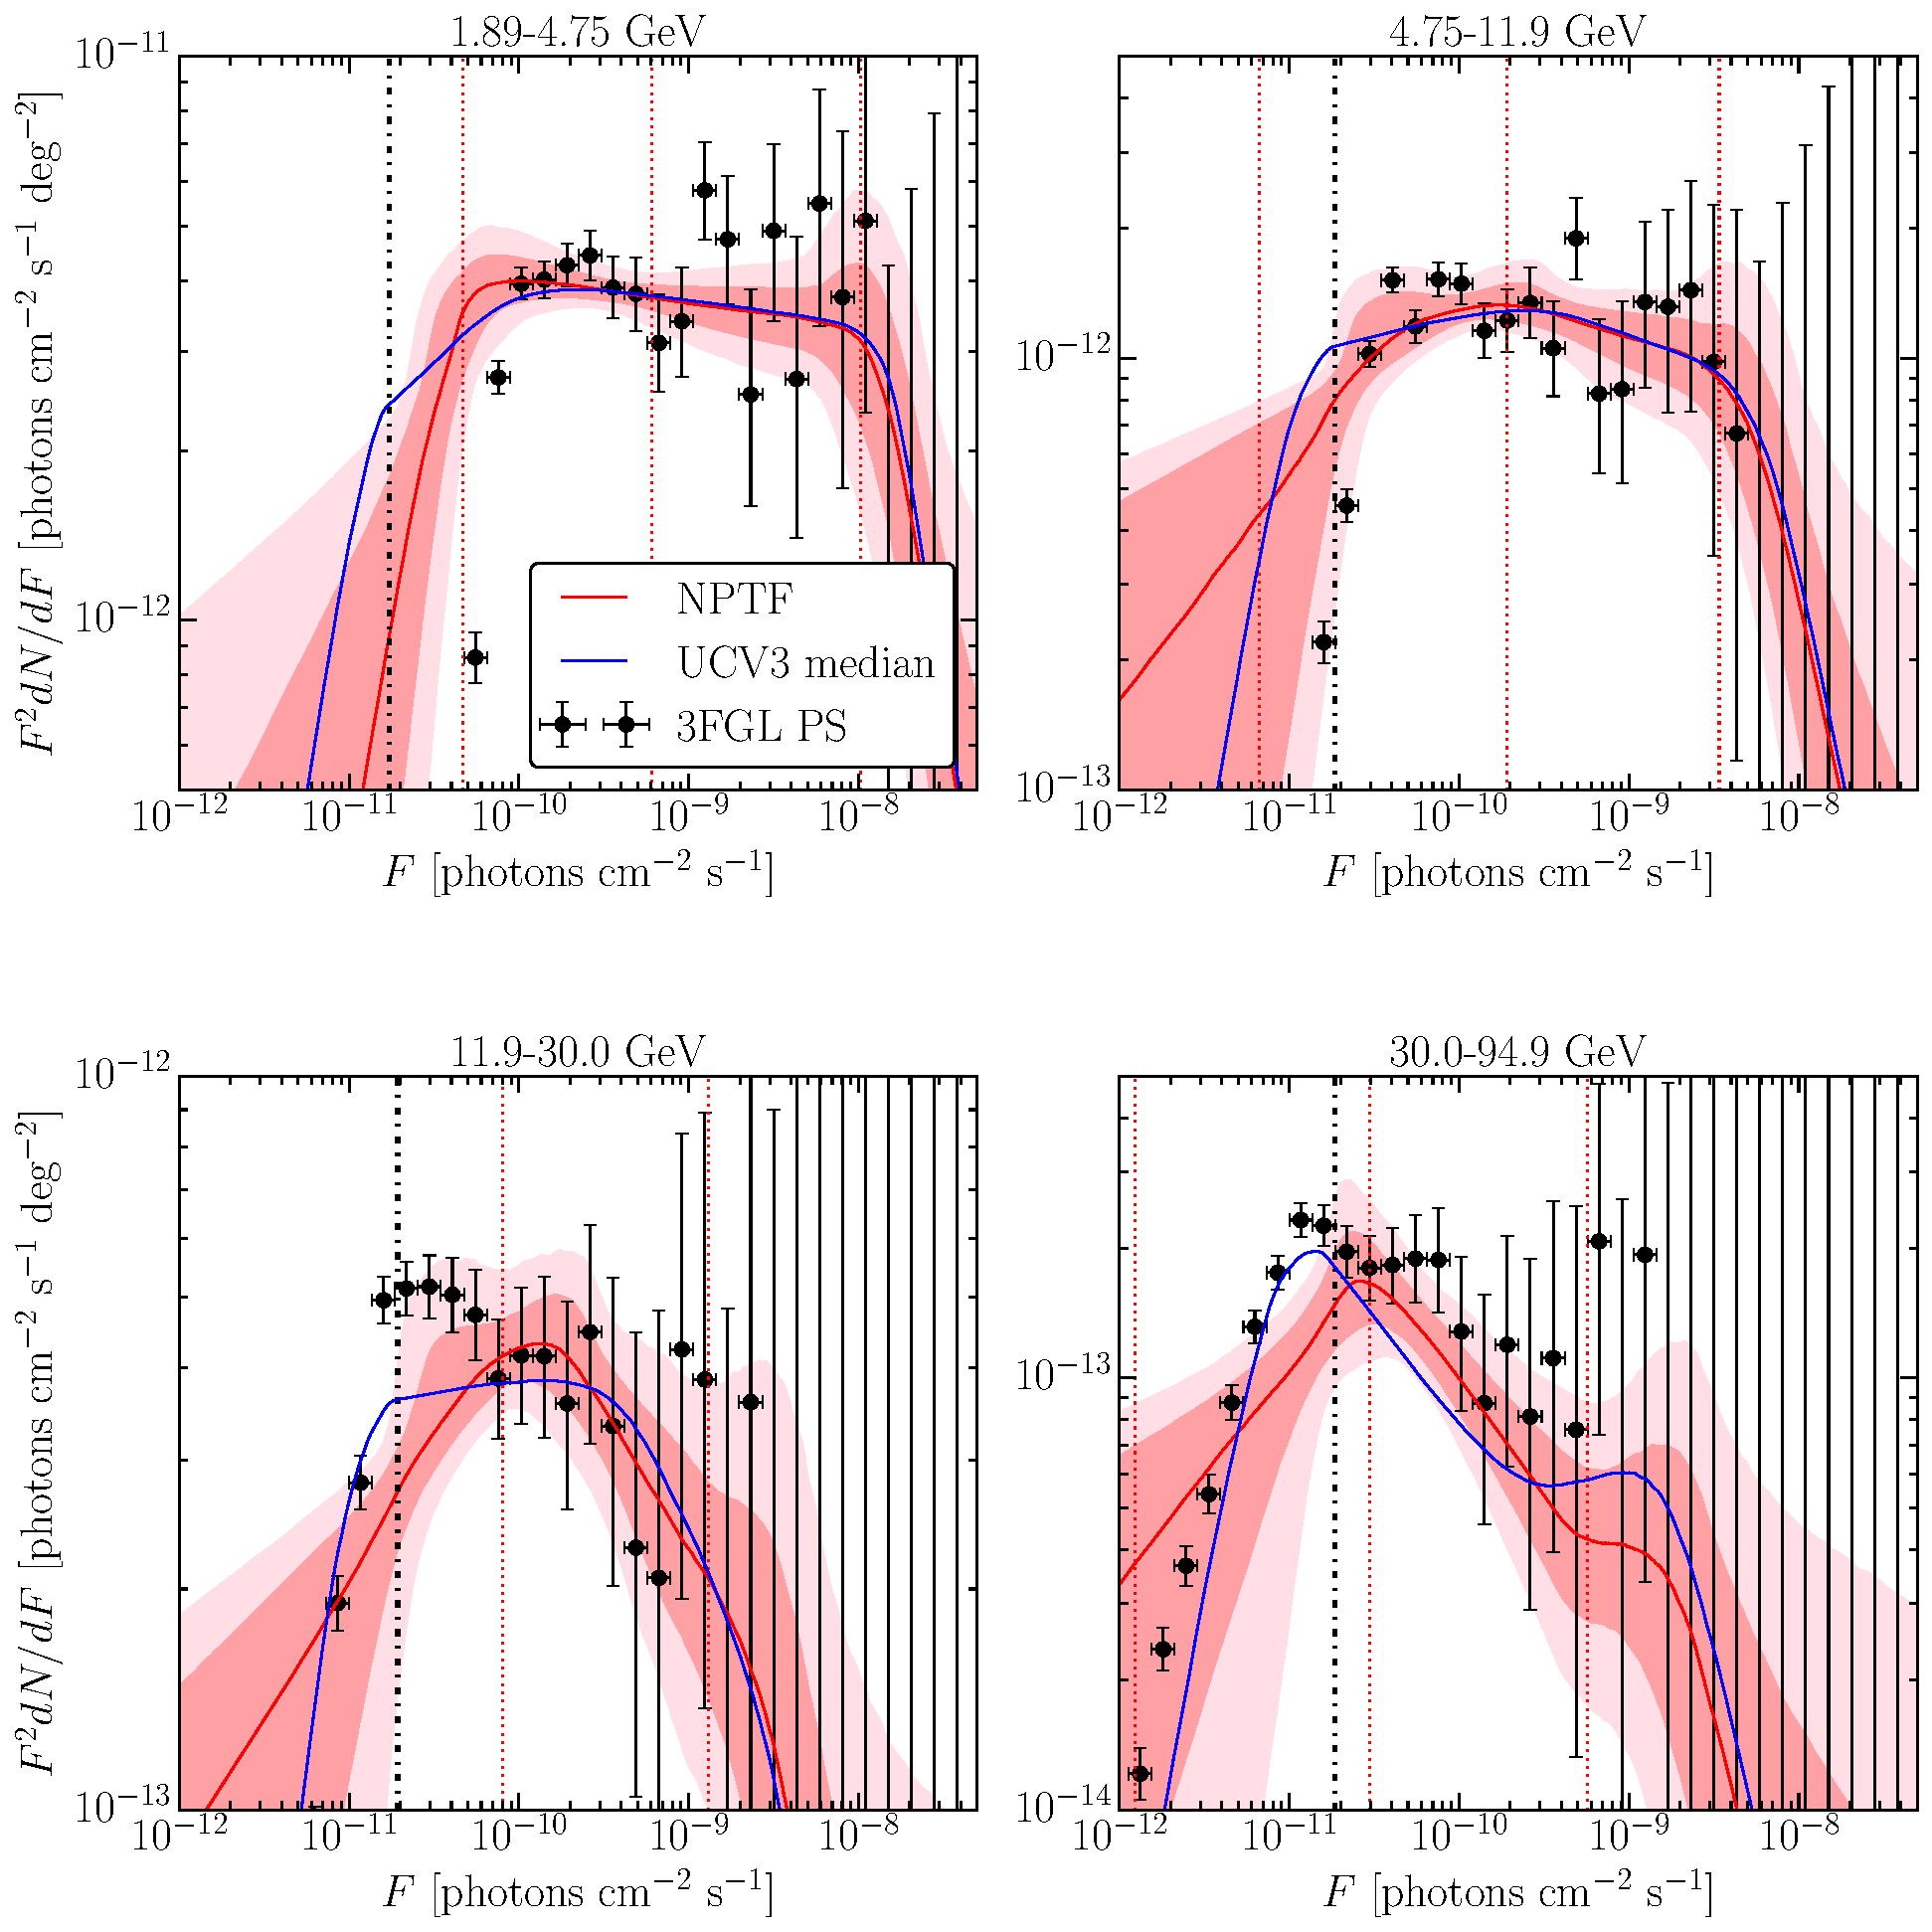
\includegraphics[width=\textwidth]{ch-igrb/plots/UCV_p8_altpriors1-dnds.pdf} 
%    \caption{Best-fit source-count distribution using the Pass 8 {\it ultracleanveto} PSF3 data set and \texttt{p8r2} foreground model, but with the break priors set to $[0.1, 10], [10,40], [40, 2\times S_\text{b,max}]$~ph, where $S_\text{b,max}$ is the maximum number of photons in the 3FGL catalog in the energy bin of interest.  The median source-count distribution for the benchmark analysis is shown in  blue. (Formatted as in Fig.~\ref{fig:dndsdata}.)}
%    \label{fig:dndsdata_altpriors1}
% \end{figure*}
% \clearpage}
% \clearpage

% \afterpage{
% \begin{figure*}[phtb] %  figure placement: here, top, bottom, or page
%    \centering
%    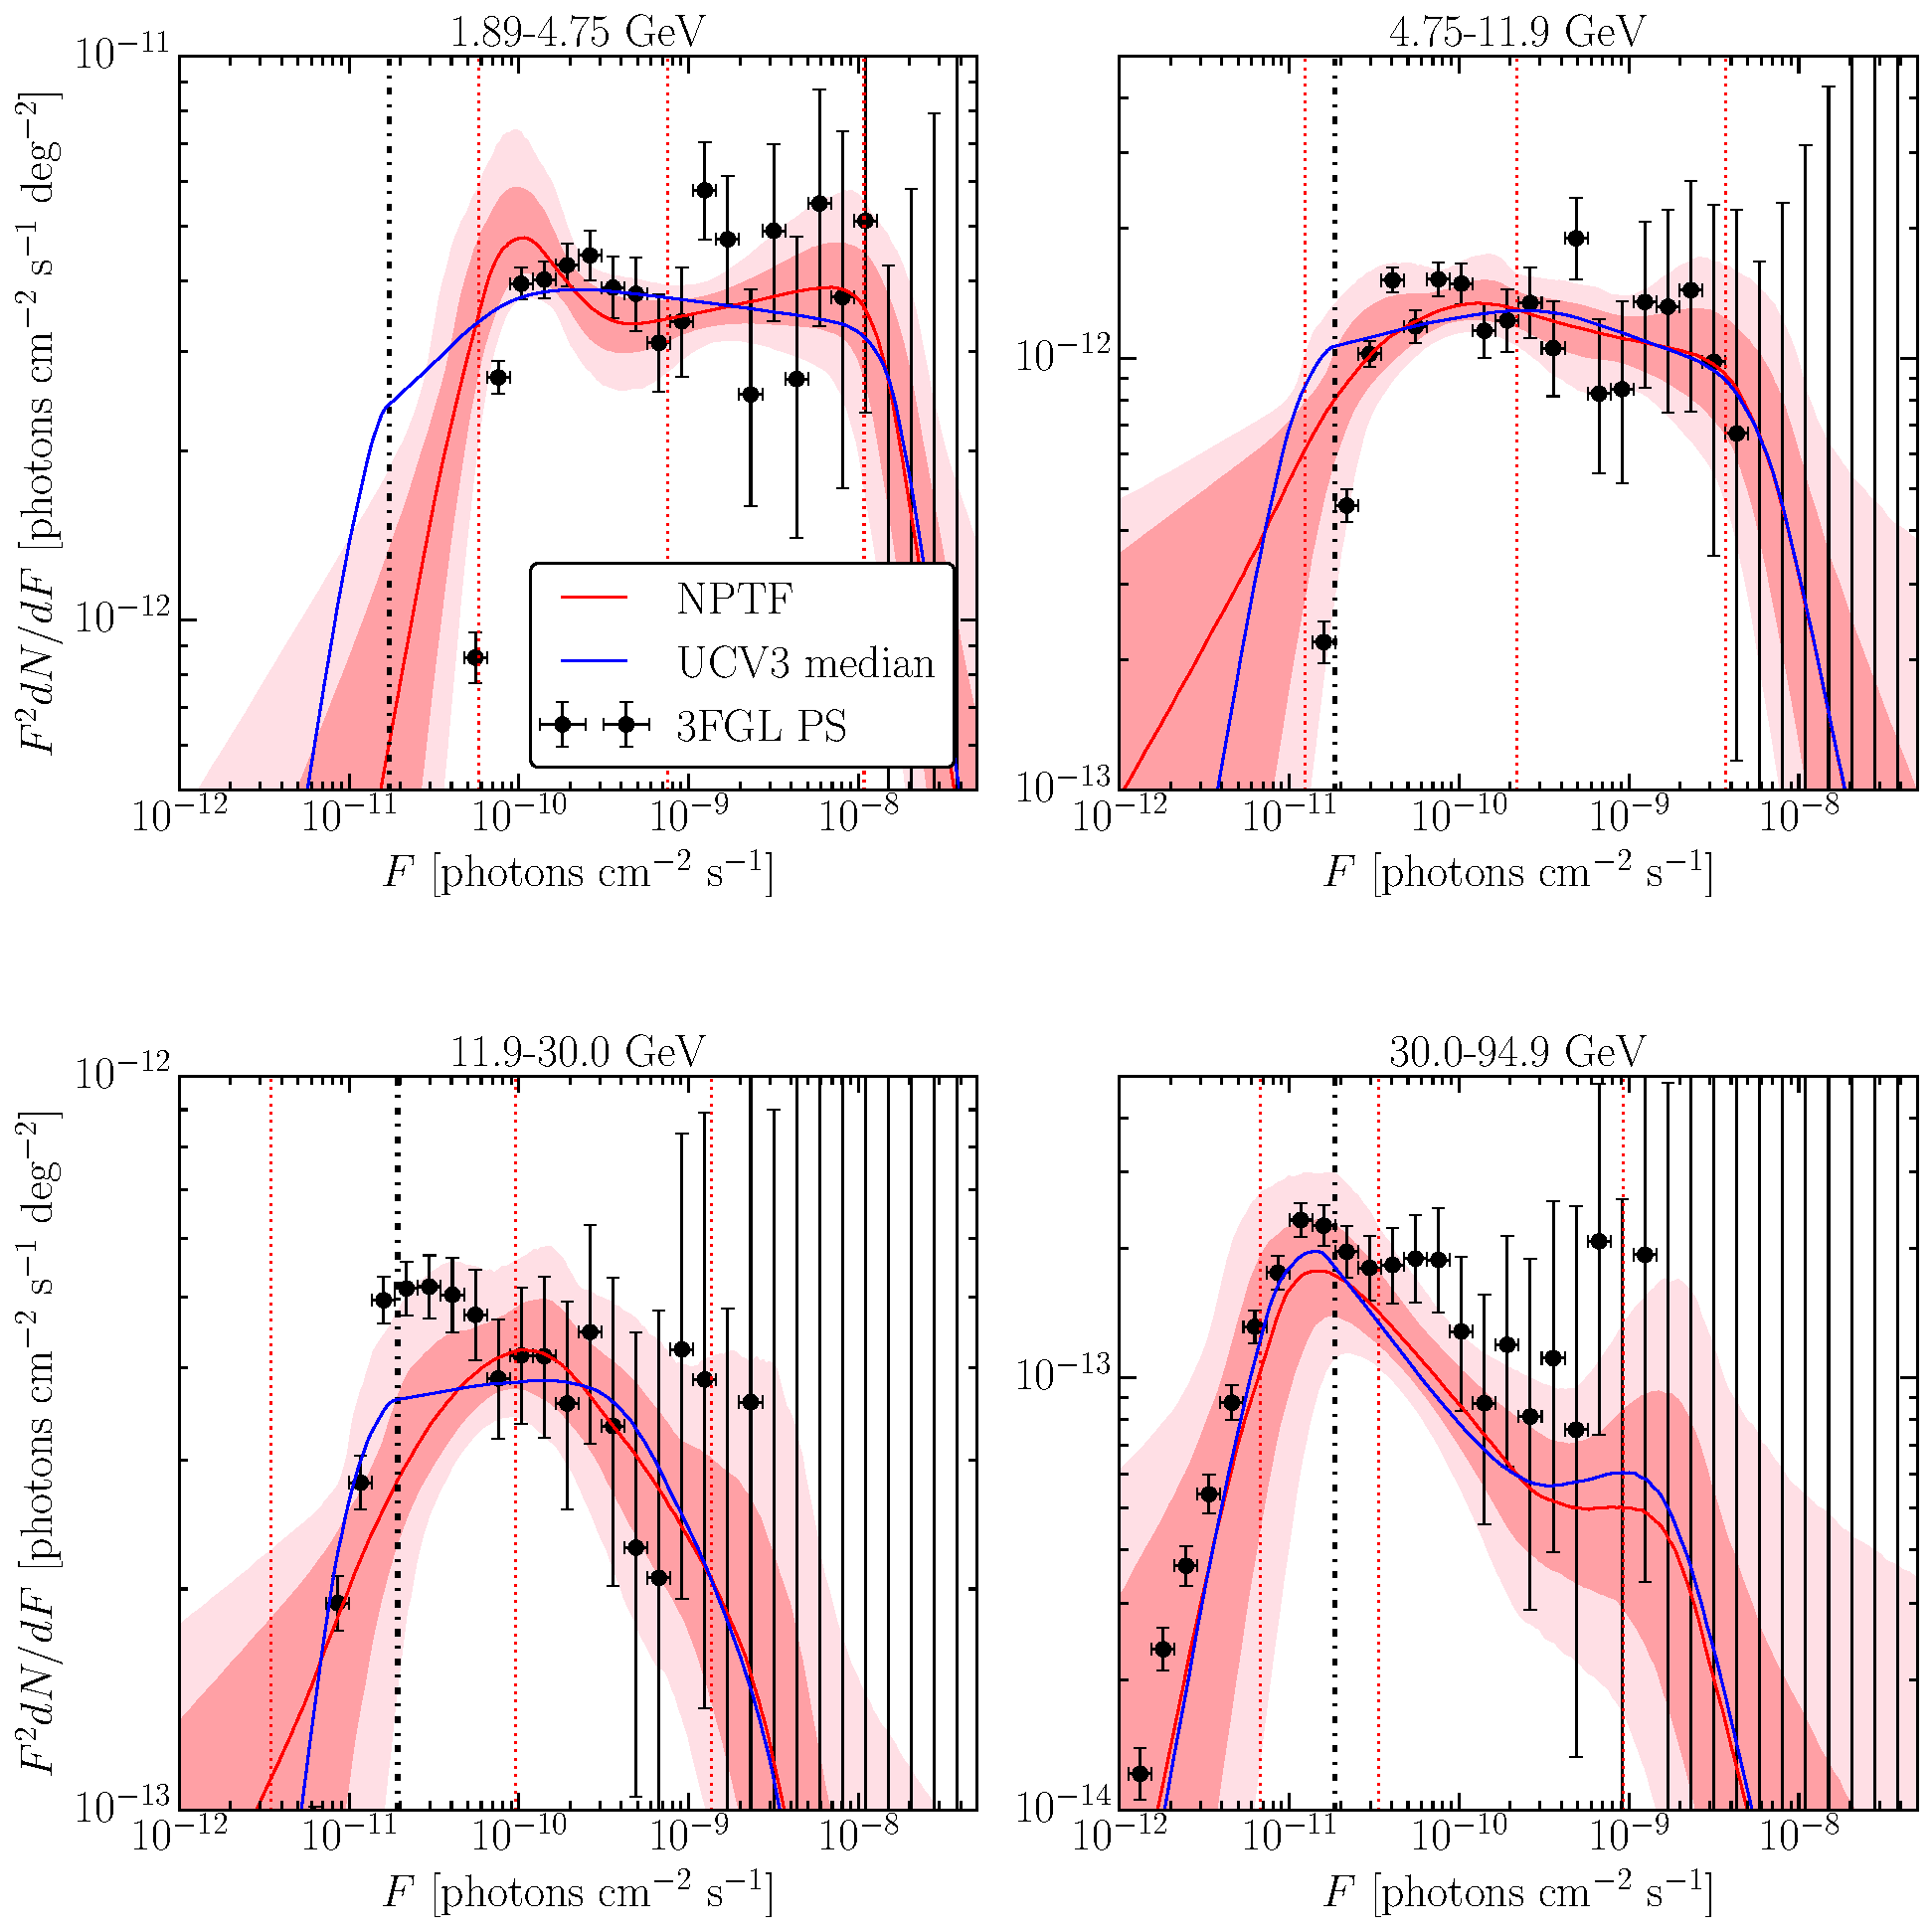
\includegraphics[width=\textwidth]{ch-igrb/plots/UCV_p8_altpriors2-dnds.pdf} 
%    \caption{Best-fit source-count distribution using the Pass 8 {\it ultracleanveto} PSF3 data set and \texttt{p8r2} foreground model, but with the break priors set to $[1, 20], [20, S_\text{b,max}/2], [S_\text{b,max}/2, 2\times S_\text{b,max}]$~ph, where $S_\text{b,max}$ is the maximum number of photons in the 3FGL catalog in the energy bin of interest.  The median source-count distribution for the benchmark analysis is shown in blue.  (Formatted as in Fig.~\ref{fig:dndsdata}.)}
%    \label{fig:dndsdata_altpriors2}
% \end{figure*}
% \clearpage}
% \clearpage

% \afterpage{
% \begin{figure*}[phtb] %  figure placement: here, top, bottom, or page
%    \centering
%    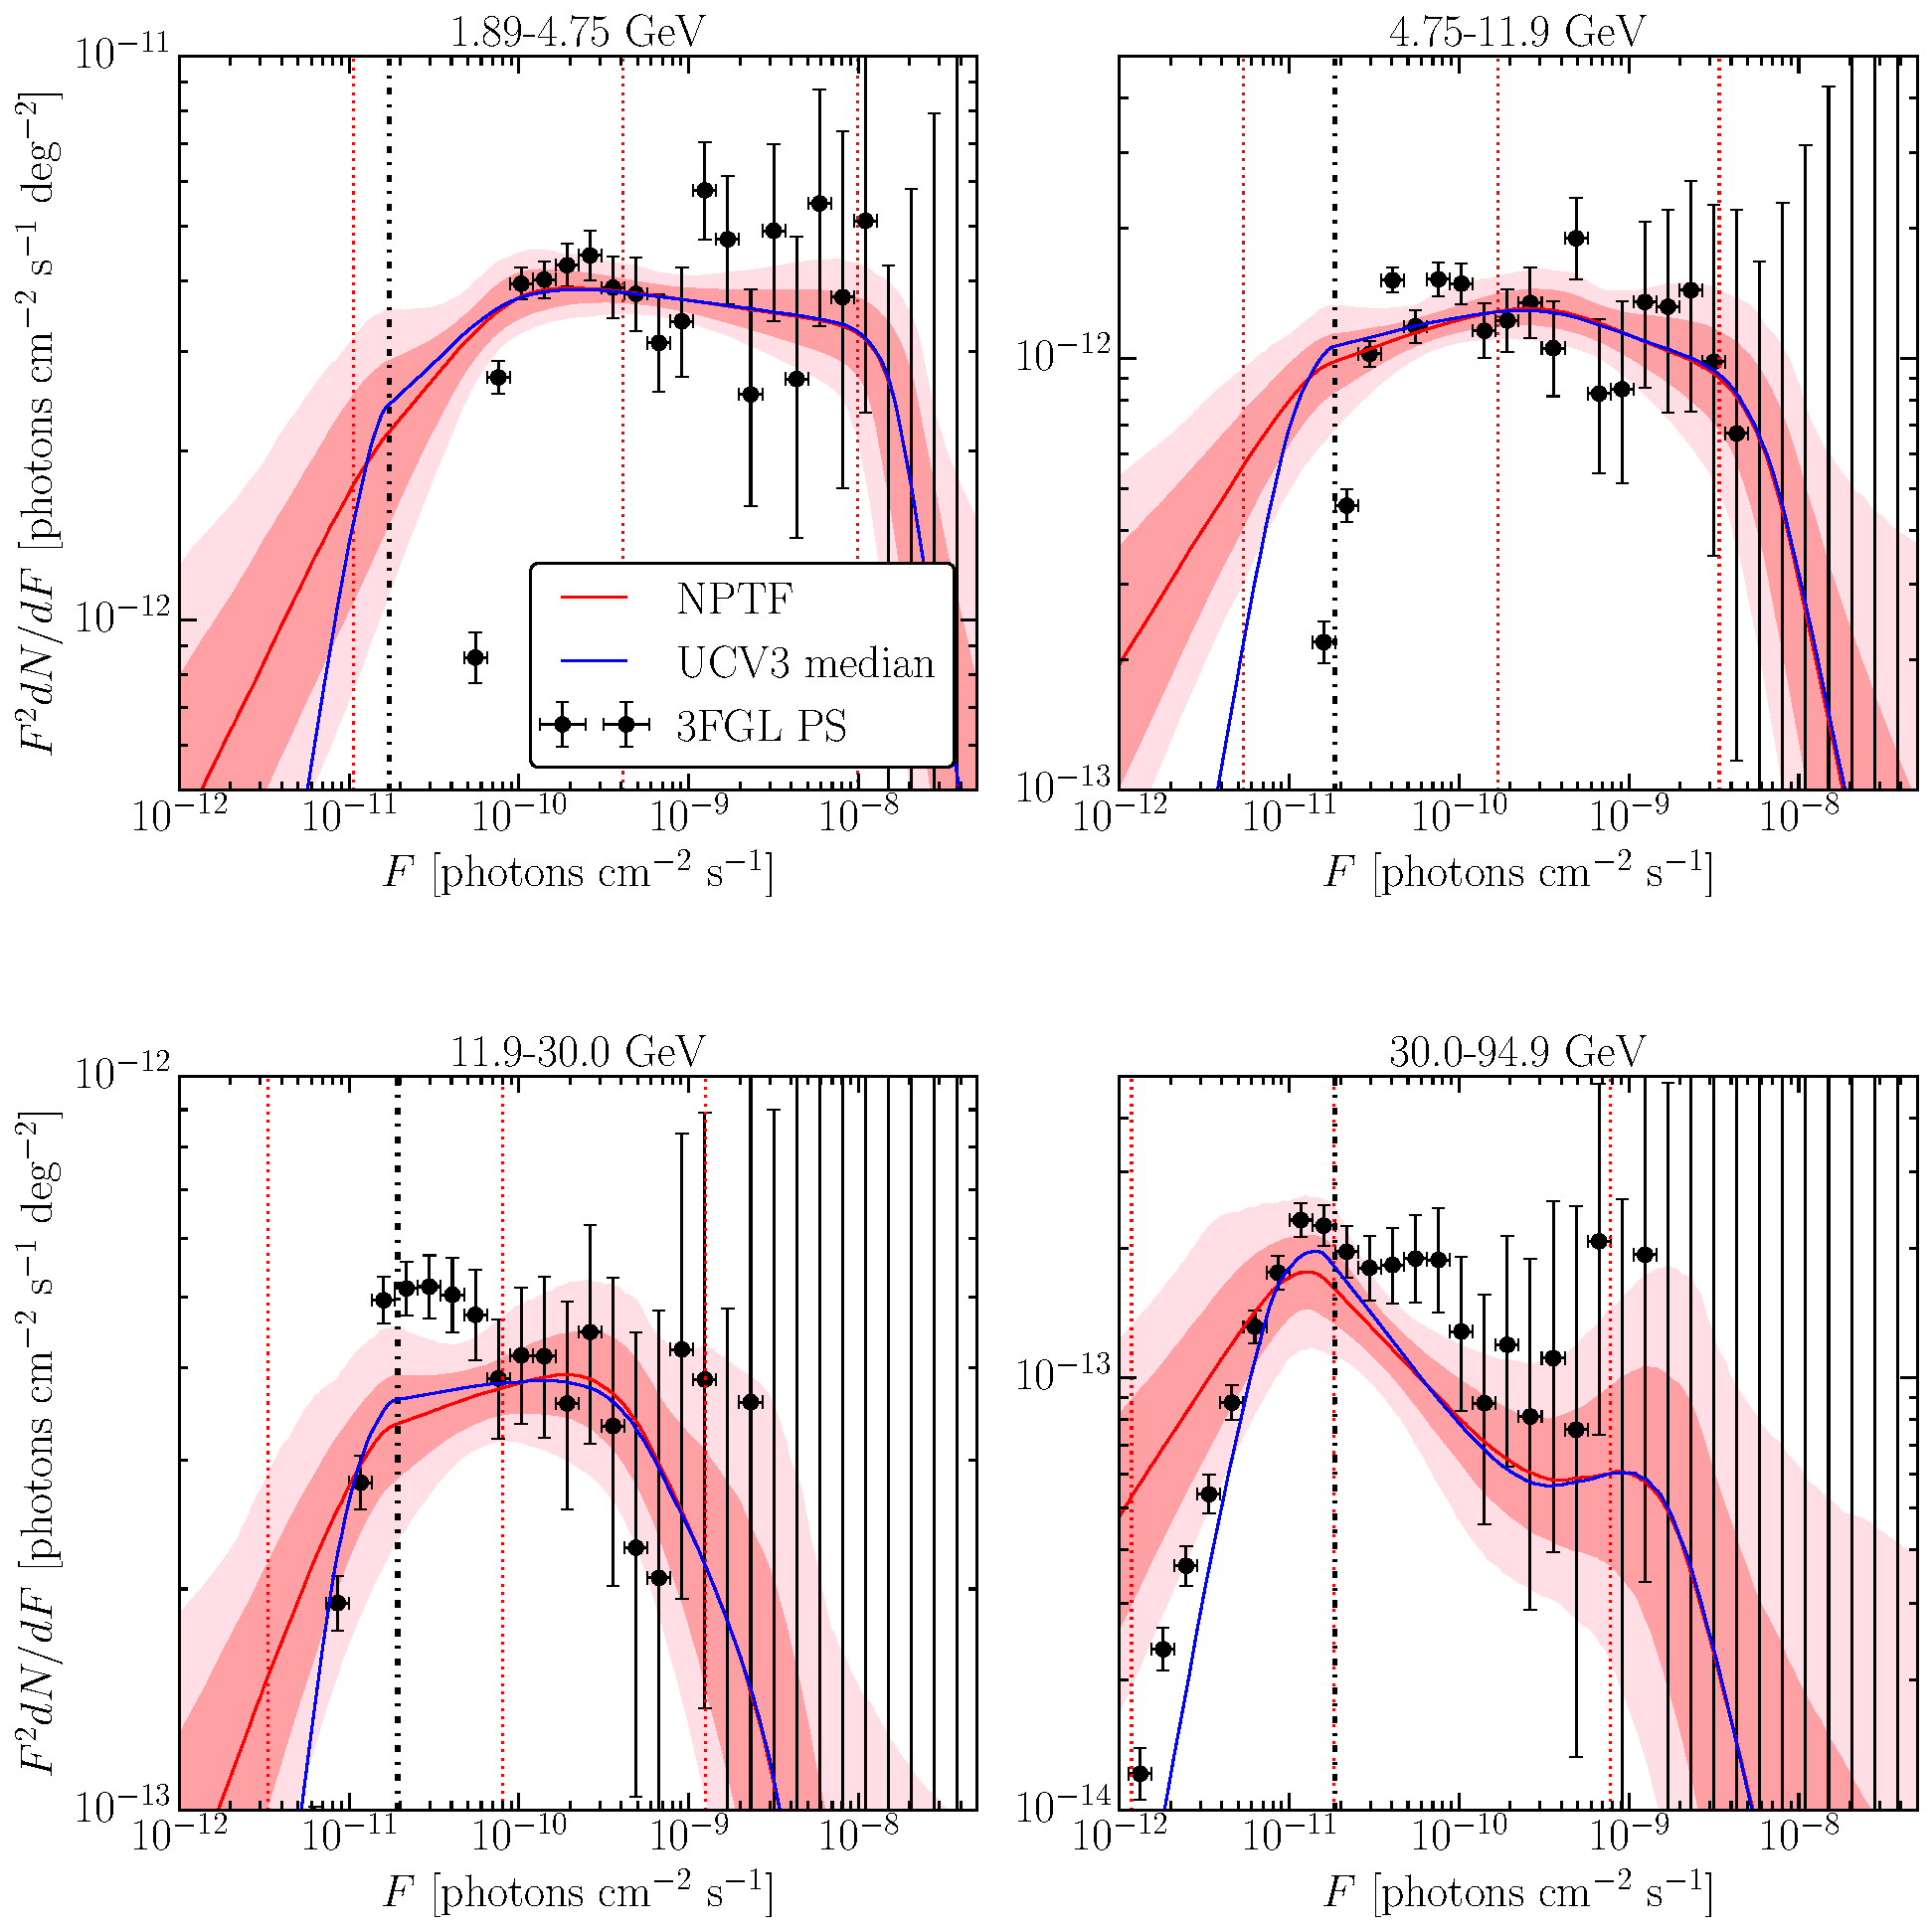
\includegraphics[width=\textwidth]{ch-igrb/plots/UCV_p8_altpriors3-dnds.pdf} 
%    \caption{Best-fit source-count distribution using the Pass 8 {\it ultracleanveto} PSF3 data set and \texttt{p8r2} foreground model, but with the prior for the lowest slope restricted to $n_{4}\in[1,2]$.  The median source-count distribution for the benchmark analysis is shown in blue. (Formatted as in Fig.~\ref{fig:dndsdata}.)}
%    \label{fig:dndsdata_altpriors3}
% \end{figure*}
% \clearpage}
% \clearpage

% \section{Supplementary Results:  High-Energy Analysis}
% \label{app:suppanalysis_high}

% This section includes supplementary information pertaining to the high-energy analysis presented in Sec.~\ref{sec:highenergy}.  In particular, Tabs.~\ref{tab:bestfit_highE_intensity} and~\ref{tab:bestfit_highE_dnds} present the best-fit intensities and source-count parameters for the NPTF analysis of all quartiles of {\it ultracleanveto} data.  Figures~\ref{fig:dndsdata_HE_m30}--\ref{fig:dndsdata_HE_S_m30} show the best-fit source-count distributions for the various systematic studies described in the text.

% \vspace{0.5in}


% \begin{table}[hpbt]
% \renewcommand{\arraystretch}{1.4}
% \setlength{\tabcolsep}{5pt}
% \begin{center}
% \begin{tabular}{ c  | c  c  c c  c   }
%  Energy & $I_\text{EGB}$&$I_\text{iso}^\text{PS}$ & $I_\text{iso}$ & $I_\text{diff}$ & $I_\text{bub}$   \\
% $[\text{GeV}]$ &  \multicolumn{5}{c}{$\left[\text{cm}^{-2}\text{ s}^{-1}\text{ sr}^{-1}\right]$}    \\
% \hline
% %\hline
% 50.0--151 
% &  $3.10_{-0.11}^{+0.13} \times 10^{-9}$ & $1.36_{-0.16}^{+0.19} \times 10^{-9}$ & $1.74_{-0.16}^{+0.13} \times 10^{-9}$ & $2.69_{-0.06}^{+0.06} \times 10^{-9}$ & $5.26_{-2.51}^{+2.60} \times 10^{-10}$\\
% % \hline
% 151--457 &    
% $4.38_{-0.32}^{+0.42} \times 10^{-10}$ & $1.56_{-0.29}^{+0.42} \times 10^{-10}$ & $2.80_{-0.31}^{+0.27} \times 10^{-10}$ & $4.12_{-0.23}^{+0.21} \times 10^{-10}$ & $5.40_{-3.81}^{+7.15} \times 10^{-11}$   \\
% % \hline
% 457--2000  & 
% $1.10_{-0.13}^{+0.15} \times 10^{-10}$ & $1.29_{-0.61}^{+0.99} \times 10^{-11}$ & $9.61_{-1.40}^{+1.32} \times 10^{-11}$ & $6.29_{-1.37}^{+1.22} \times 10^{-11}$ & $7.18_{-4.11}^{+5.02} \times 10^{-11}$  \\  
% % \hline
% 50.0-2000  &  
% $3.74_{-0.12}^{+0.16} \times 10^{-9}$ & $1.61_{-0.18}^{+0.22} \times 10^{-9}$ & $2.13_{-0.19}^{+0.15} \times 10^{-9}$ & $3.29_{-0.07}^{+0.07} \times 10^{-9}$ & $5.26_{-2.58}^{+3.01} \times 10^{-10}$ \\
% \end{tabular}
% \end{center}
% \caption{Same as Tab.~\ref{tab:bestfit}, except using all quartiles (PSF0--3) of the Pass~8 {\it ultracleanveto} data for the high-energy analysis.  Note that the \emph{Fermi} bubbles template intensity is defined relative to the interior of the bubbles, while the intensities of the other templates are computed with respect to the region $|b| > 10^\circ$.  }
% \label{tab:bestfit_highE_intensity}
% \end{table}

% \vspace{0.5in}

% \begin{table}[hpbt]
% \renewcommand{\arraystretch}{1.4}
% \setlength{\tabcolsep}{3pt}
% \begin{center}
% \begin{tabular}{ c  | c  c  c c |  c c c   }
%  Energy & $n_1$ & $n_2$ & $n_3$ & $n_4$ & $F_{b,3}$ & $F_{b,2}$ & $F_{b,1}$   \\
% $[\text{GeV}]$ &  & & & & \multicolumn{3}{c}{$\left[\text{cm}^{-2}\text{ s}^{-1}\right]$}    \\
% \hline
% %\hline
% 50.0--151 &  
% $3.56_{-0.90}^{+0.92}$ & $2.34_{-0.27}^{+0.36}$ & $2.18_{-0.11}^{+0.12}$ & $-0.05_{-1.21}^{+1.12}$ & $1.58_{-0.76}^{+1.21} \times 10^{-12}$ & $7.93_{-4.10}^{+2.78} \times 10^{-11}$ & $1.55_{-0.73}^{+0.77} \times 10^{-9}$
%    \\
% % \hline
% 151--457 &    
% $3.56_{-0.97}^{+0.95}$ & $1.87_{-0.53}^{+0.65}$ & $2.42_{-0.28}^{+0.39}$ & $-0.06_{-1.26}^{+1.08}$ & $2.53_{-1.15}^{+1.16} \times 10^{-12}$ & $6.41_{-3.86}^{+4.34} \times 10^{-11}$ & $4.80_{-2.29}^{+2.63} \times 10^{-10}$
%    \\
% % \hline
% 457--2000  & 
% $3.57_{-0.96}^{+0.91}$ & $2.26_{-0.78}^{+0.78}$ & $2.16_{-0.67}^{+0.68}$ & $-0.01_{-1.25}^{+1.25}$ & $3.16_{-1.68}^{+1.74} \times 10^{-12}$ & $8.90_{-5.73}^{+5.94} \times 10^{-11}$ & $2.35_{-0.37}^{+0.38} \times 10^{-10}$
%   \\  
% % \hline
% 50.0-2000  &  
% $3.63_{-0.99}^{+0.90}$ & $2.28_{-0.22}^{+0.28}$ & $2.17_{-0.09}^{+0.12}$ & $-0.05_{-1.24}^{+1.10}$ & $1.72_{-0.79}^{+1.29} \times 10^{-12}$ & $7.87_{-4.37}^{+3.16} \times 10^{-11}$ & $2.15_{-1.06}^{+1.18} \times 10^{-9}$
%   \\
% \end{tabular}
% \end{center}
% \caption{Same as Tab.~\ref{tab:bestfit_dndf}, except using all quartiles (PSF0--3) of the Pass~8 {\it ultracleanveto} data for the high-energy analysis.  }
% \label{tab:bestfit_highE_dnds}
% \end{table}

% \afterpage{
% \begin{figure*}[phtb] %  figure placement: here, top, bottom, or page
%    \centering
%    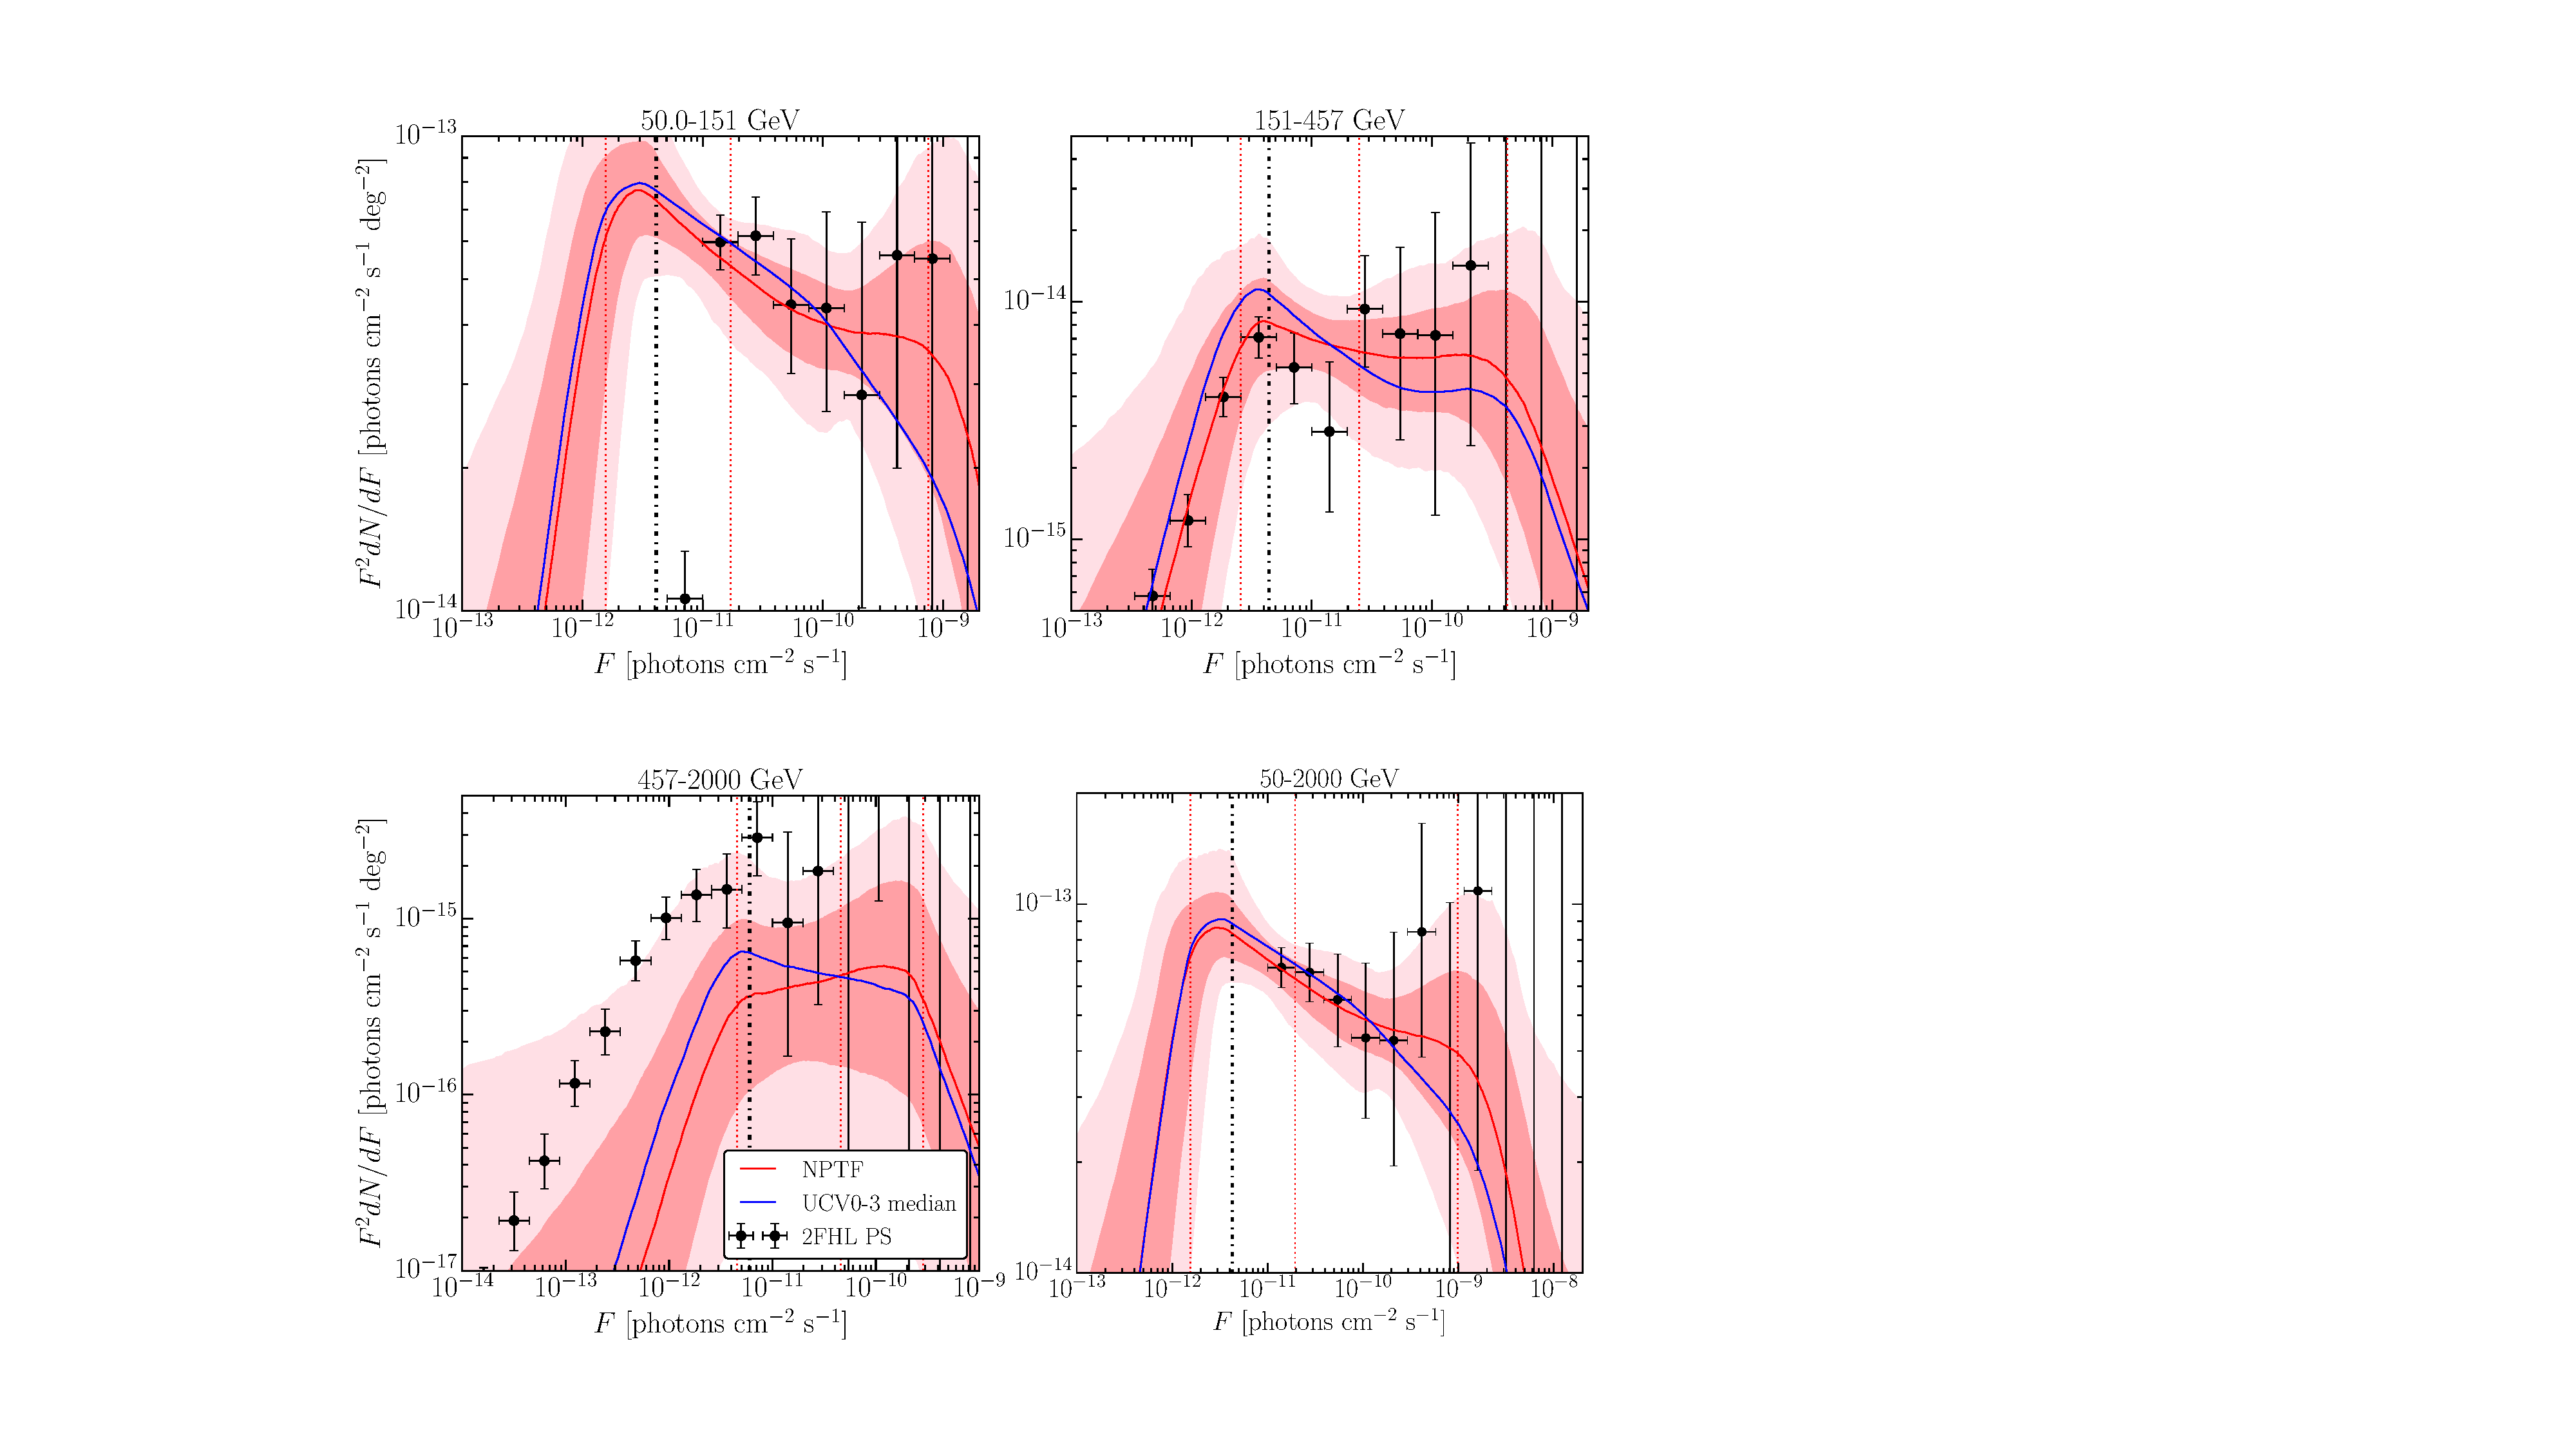
\includegraphics[width=\textwidth]{ch-igrb/plots/N128UHEp8-2K-SourceCounts-final-700-E15-p8-3br.pdf} 
%    \caption{   Best-fit source-count distribution using the Pass 8 {\it ultracleanveto} PSF0--3 data set and \texttt{p8r2} foreground model, but with $|b| > 30^\circ$.  The median source-count distribution for the benchmark analysis is shown in blue.  (Formatted as in Fig.~\ref{fig:dndsdata_HE}.)}
%    \label{fig:dndsdata_HE_m30}
% \end{figure*}
% \clearpage}

% \afterpage{
% \begin{figure*}[phtb] %  figure placement: here, top, bottom, or page
%    \centering
%    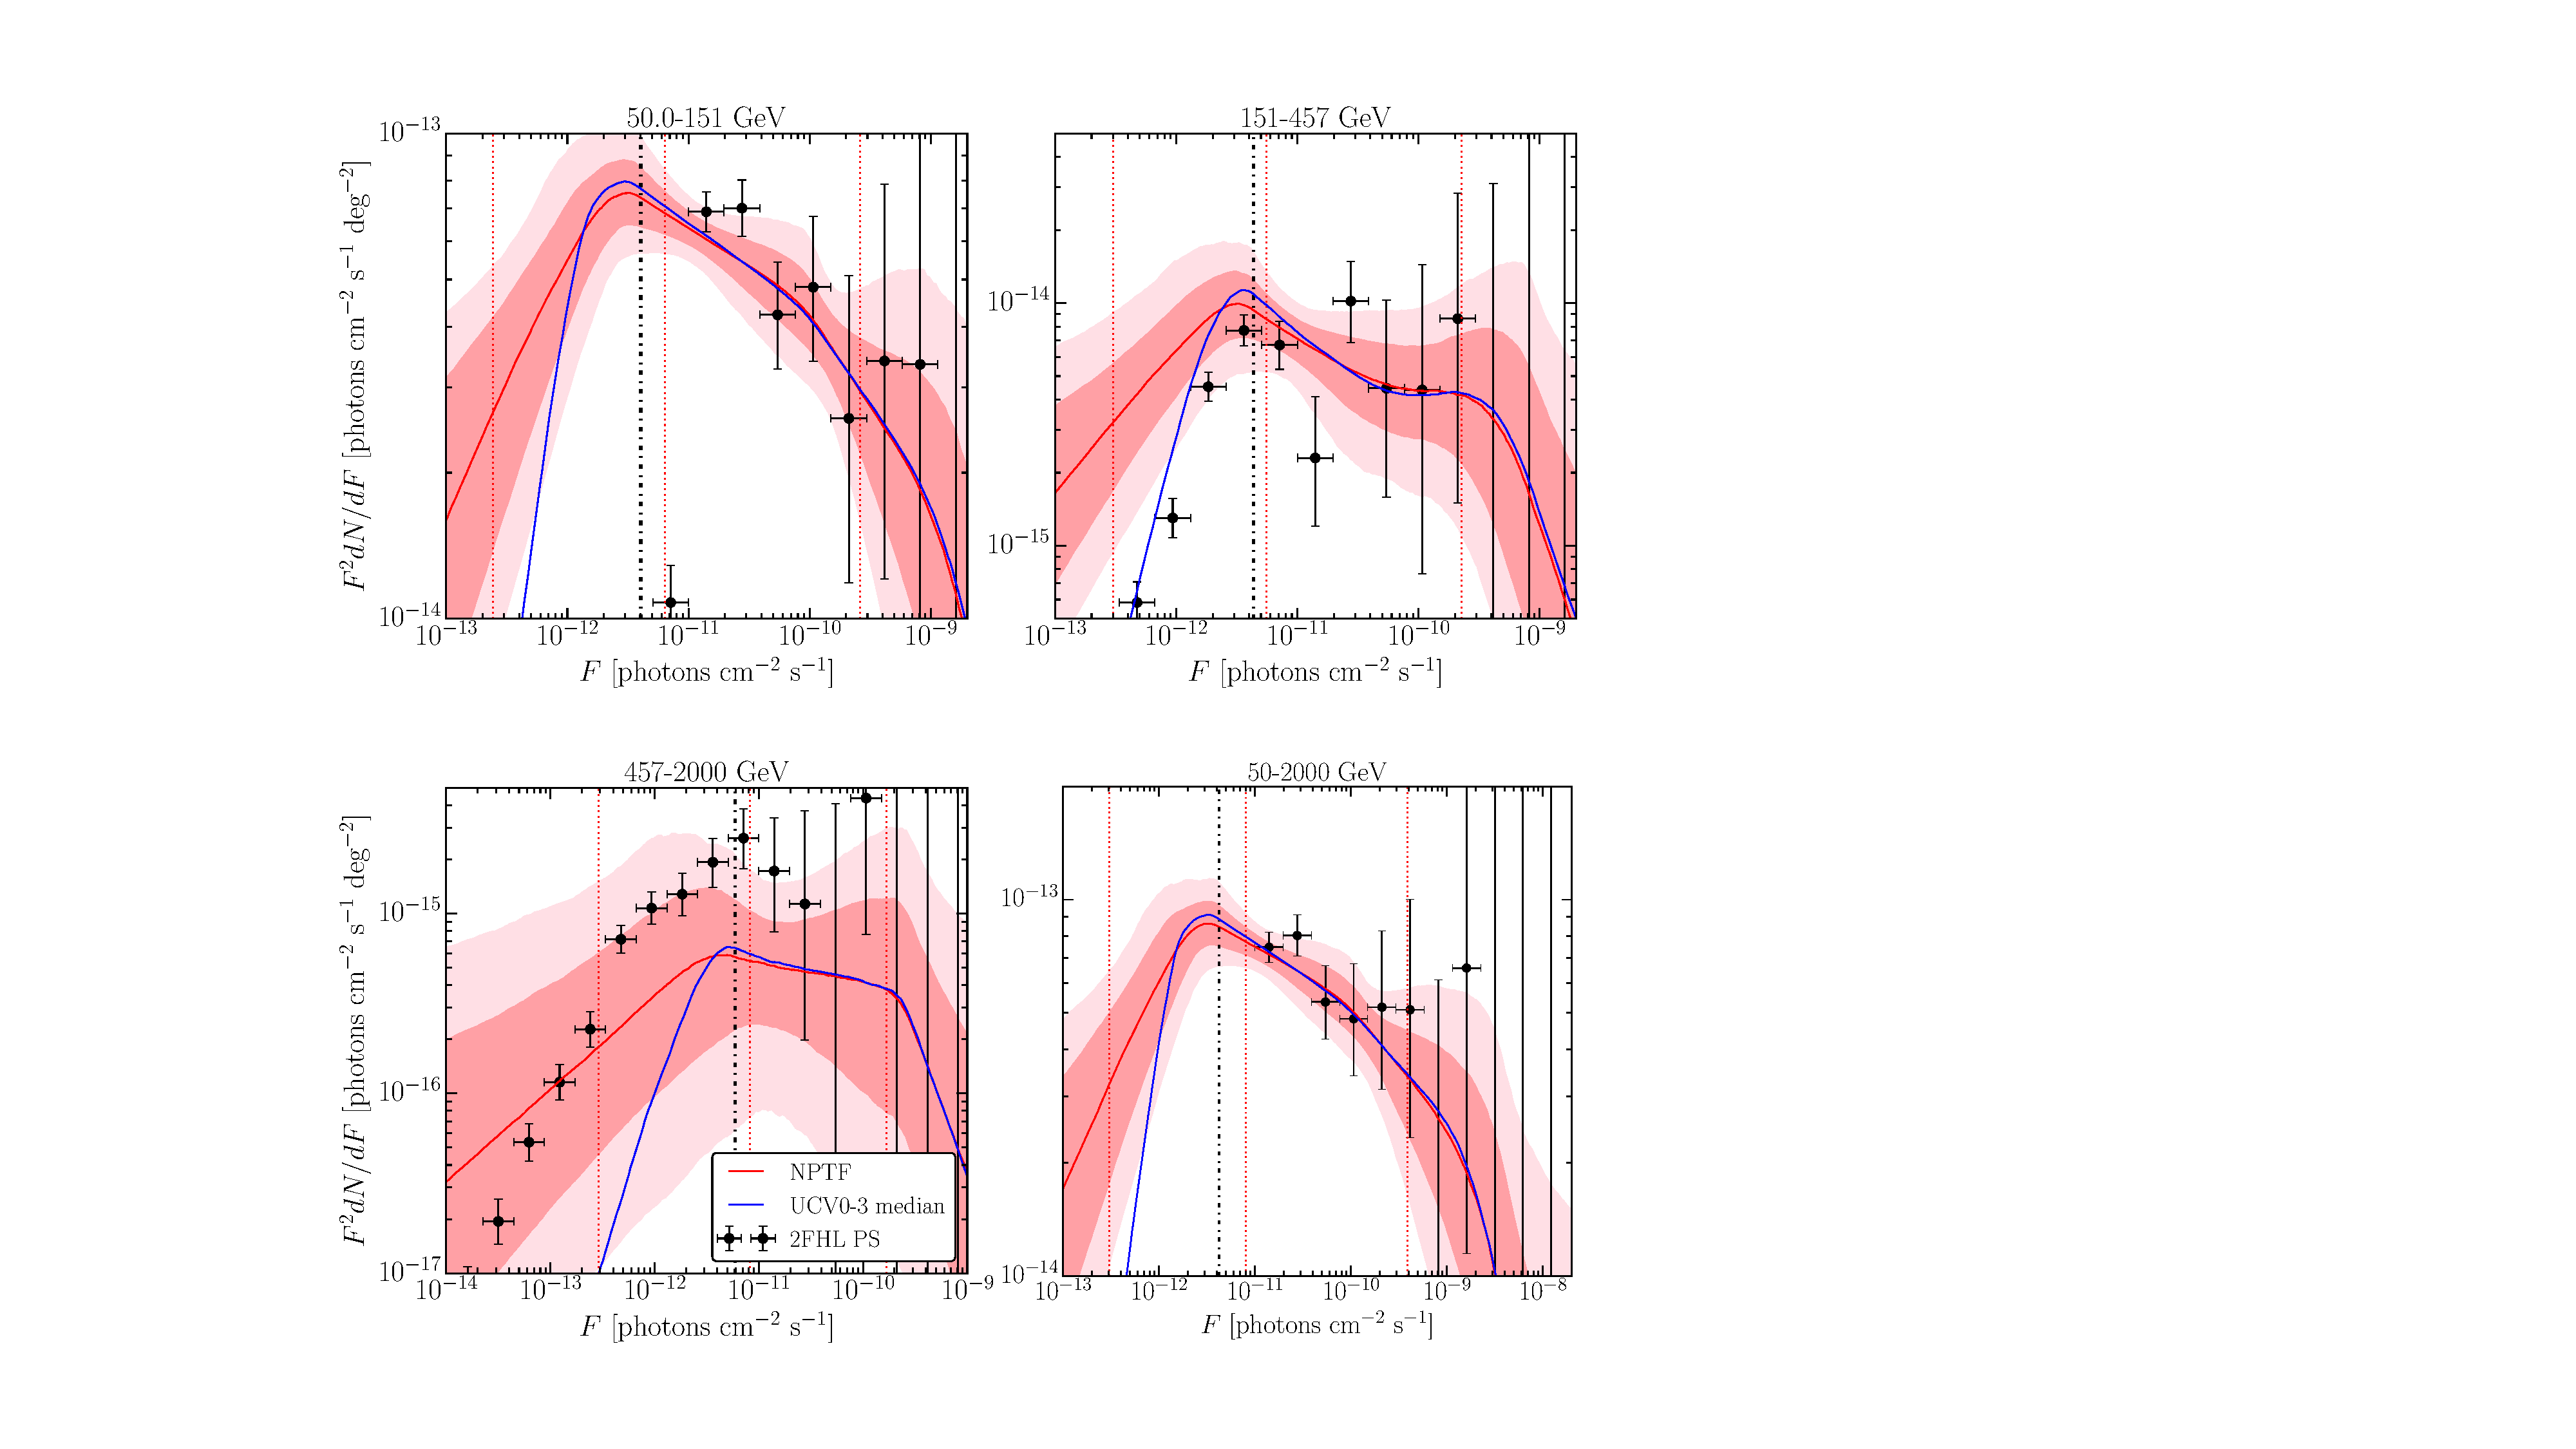
\includegraphics[width=\textwidth]{ch-igrb/plots/N128UHEp8nb1-0K-SourceCounts-final-700-E15-p8-3br.pdf} 
%    \caption{Best-fit source-count distribution using the Pass 8 {\it ultracleanveto} PSF0--3 data set and \texttt{p8r2} foreground model, but with the prior on the lowest slope restricted to $n_{4}\in[1,2]$.  The median source-count distribution for the benchmark analysis is shown in blue.  (Formatted as in Fig.~\ref{fig:dndsdata_HE}.)}
%    \label{fig:dndsdata_HE_m30}
% \end{figure*}
% \clearpage}

% \afterpage{
% \begin{figure*}[phtb] %  figure placement: here, top, bottom, or page
%    \centering
%    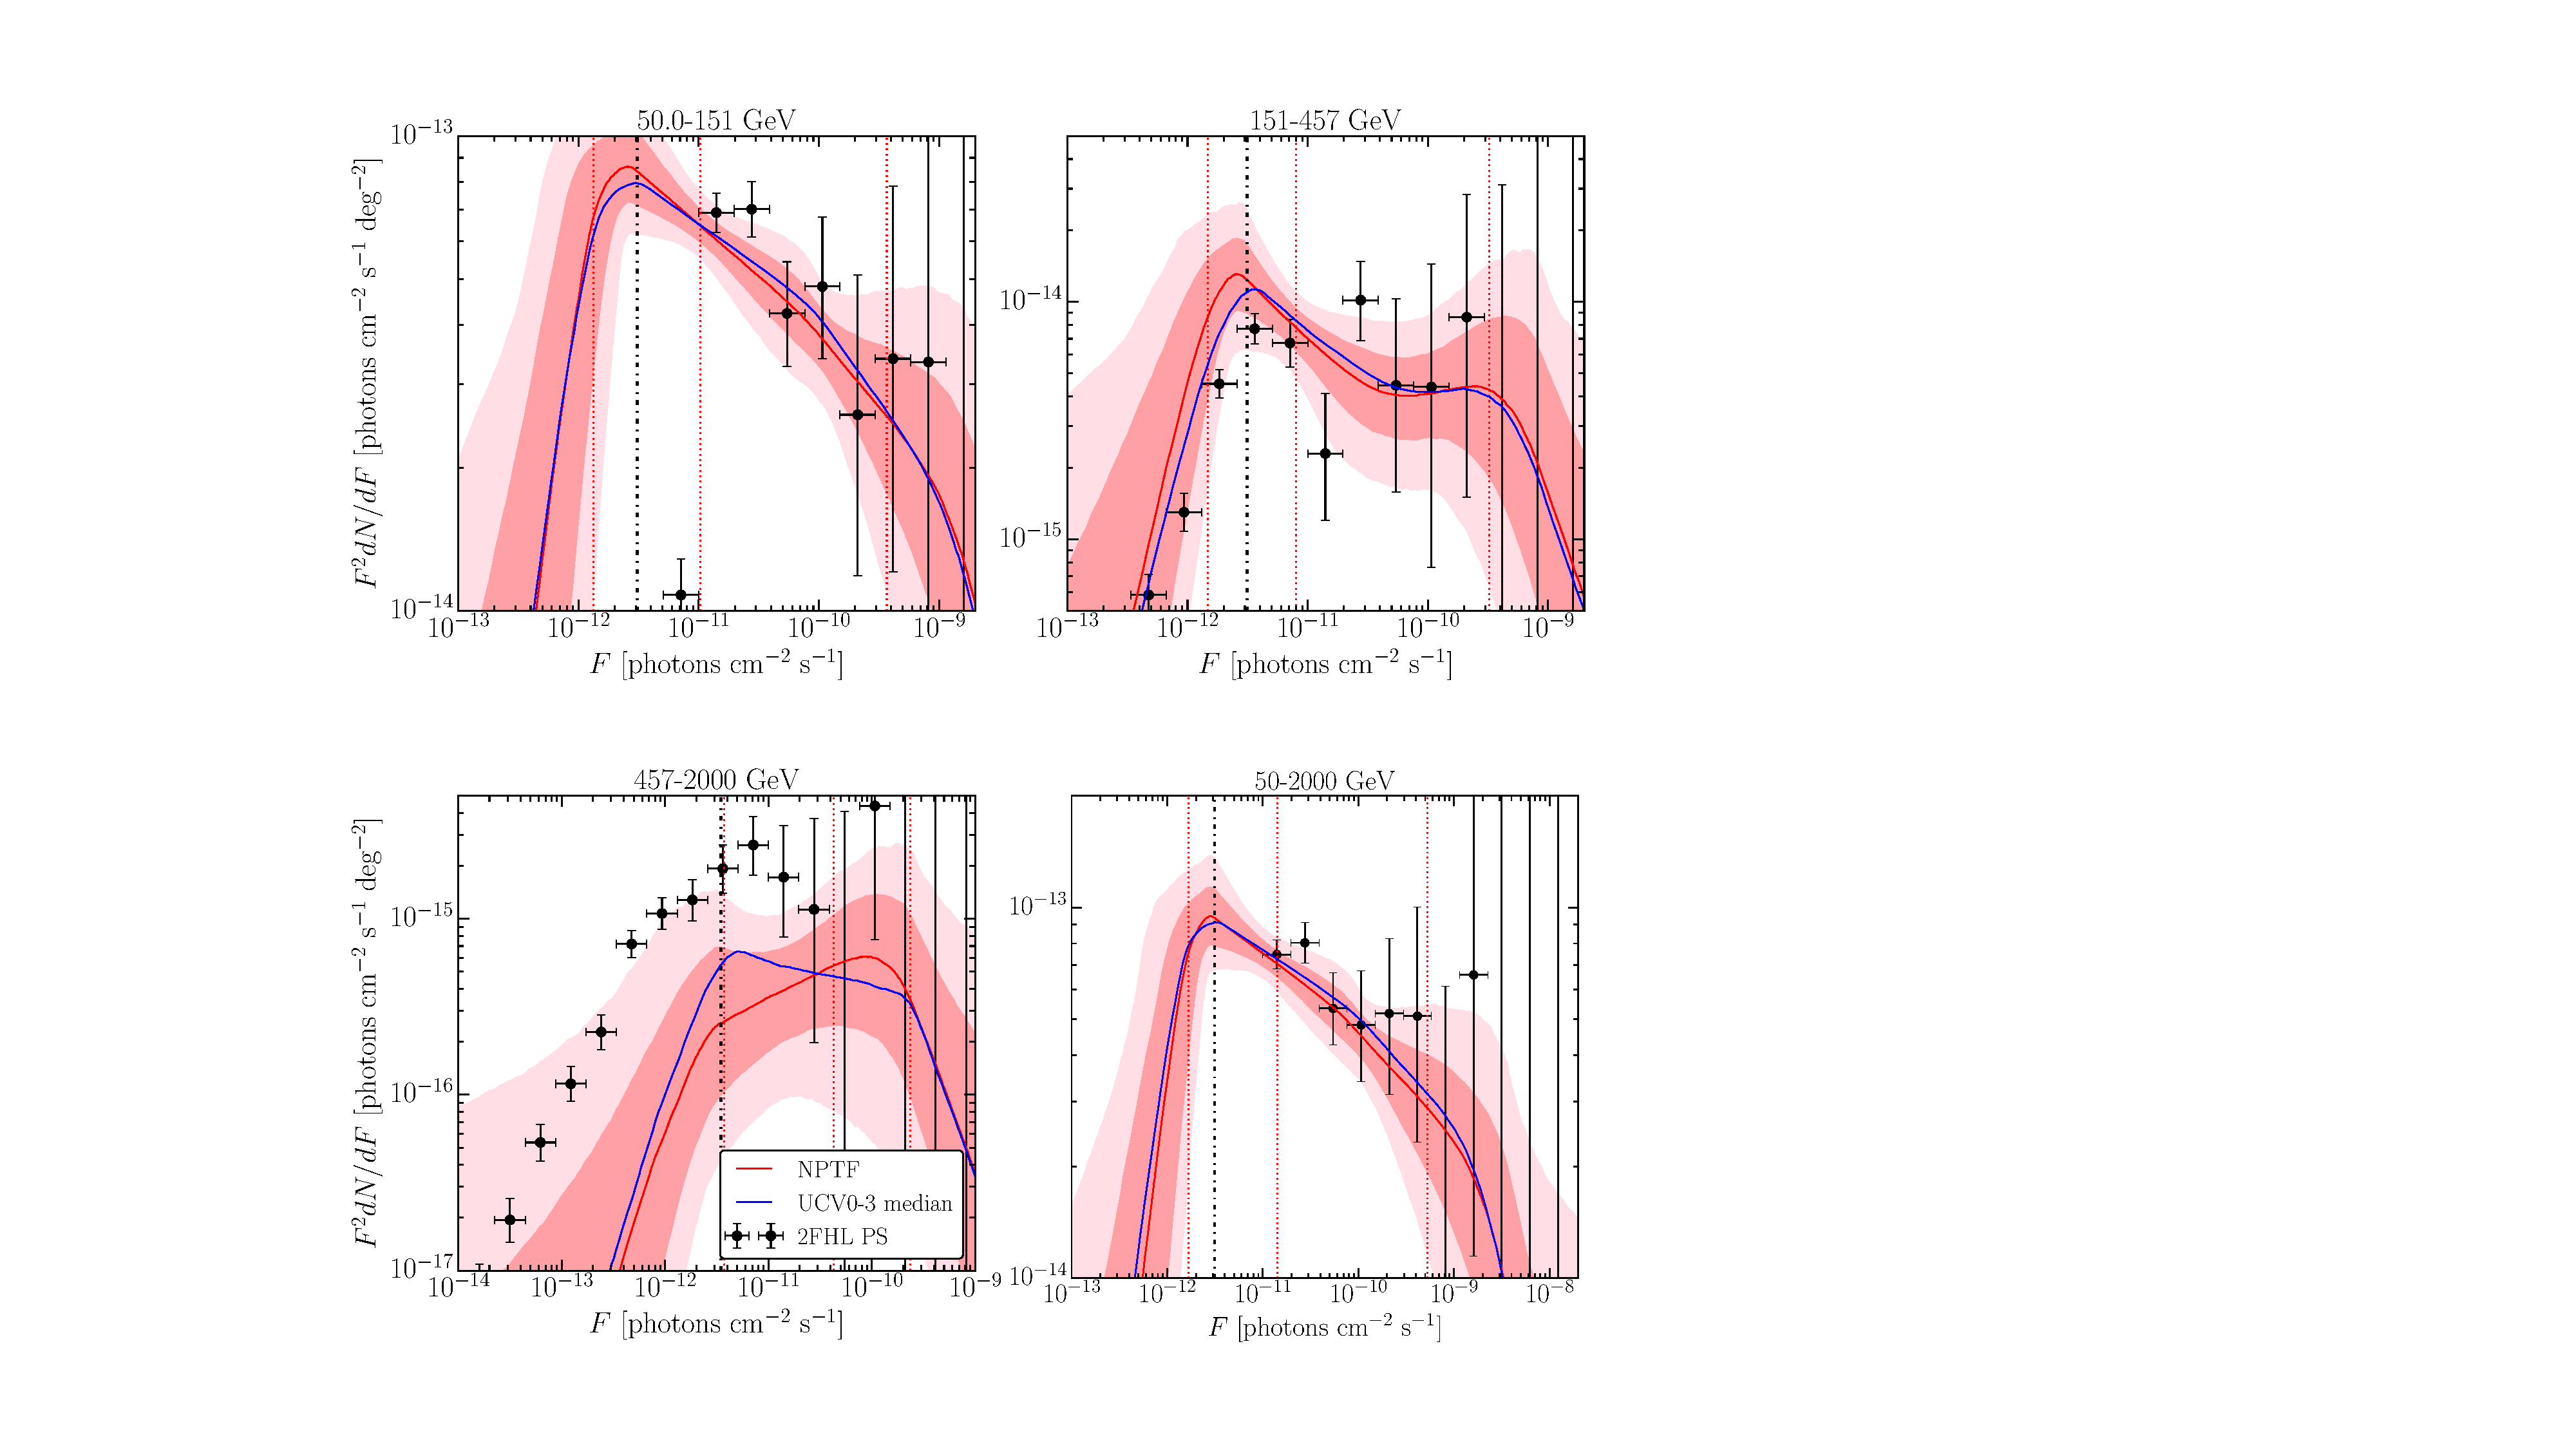
\includegraphics[width=\textwidth]{ch-igrb/plots/N128HEp8-0K-SourceCounts-final-700-E15-p8-3br} 
%    \caption{Best-fit source-count distribution using the Pass 8 {\it source} PSF0--3 data set and \texttt{p8r2} foreground model, with $|b| > 10^\circ$.  The median source-count distribution for the benchmark analysis is shown in blue.  (Formatted as in Fig.~\ref{fig:dndsdata_HE}.)}
%    \label{fig:dndsdata_HE_S_m10}
% \end{figure*}
% \clearpage}

% \afterpage{
% \begin{figure*}[phtb] %  figure placement: here, top, bottom, or page
%    \centering
%    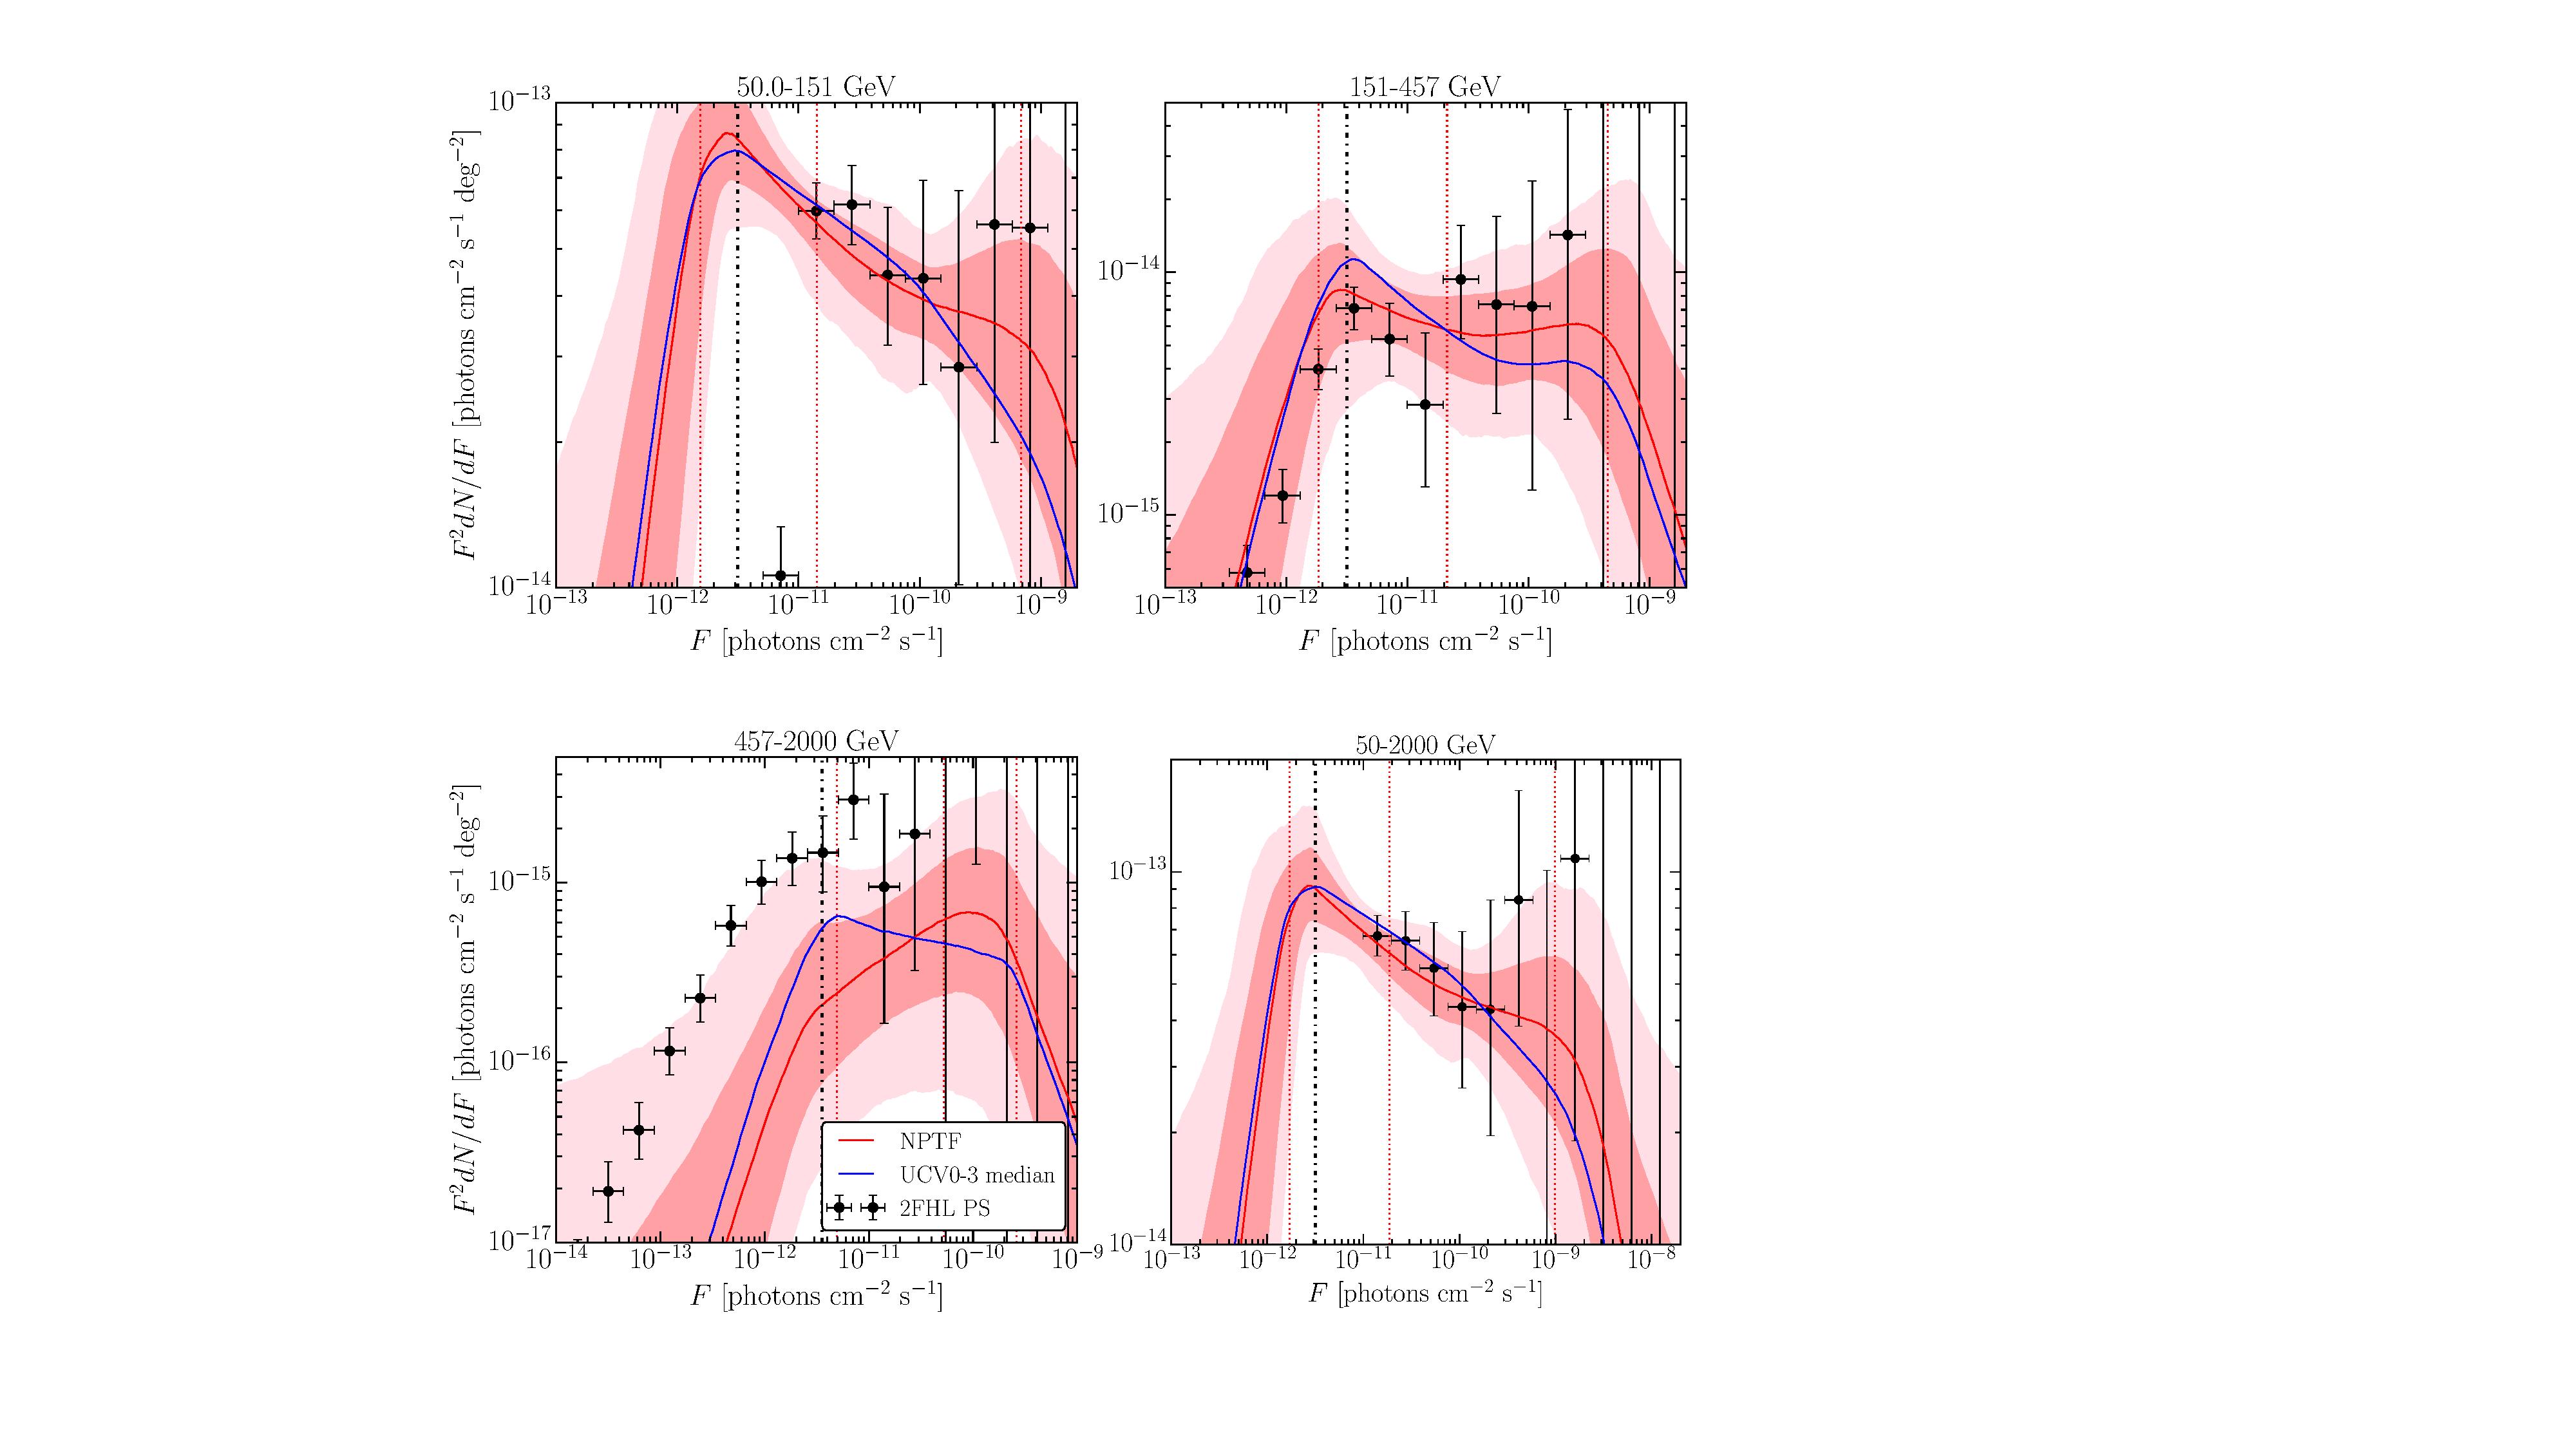
\includegraphics[width=\textwidth]{ch-igrb/plots/N128HEp8-2K-SourceCounts-final-700-E15-p8-3br} 
%    \caption{Best-fit source-count distribution using the Pass 8 {\it source} PSF0--3 data set and \texttt{p8r2} foreground model, but with $|b| > 30^\circ$.  The median source-count distribution for the benchmark analysis is shown in blue. (Formatted as in Fig.~\ref{fig:dndsdata_HE}.)}
%    \label{fig:dndsdata_HE_S_m30}
% \end{figure*}
% \clearpage}
